\documentclass[a4paper,12pt,twoside]{report}

\usepackage{graphicx}
\usepackage{subfig}
\usepackage{fancyheadings}
\usepackage{longtable}
\usepackage{amsmath,bm}
\usepackage{float}
\usepackage{bookmark}
\usepackage{subfiles}
\usepackage{datetime}
\usepackage{setspace}
\usepackage{listings}
\usepackage{xcolor}
\usepackage{hyperref}
\usepackage{multirow}
\usepackage{perpage} %the perpage package
\usepackage[perpage]{footmisc}
\usepackage{caption}
\usepackage{ragged2e}
\usepackage{algorithmic}
\usepackage{gensymb}
\usepackage{dsfont}
\usepackage{natbib}

\setlength{\bibsep}{7.3pt}


\captionsetup{font=footnotesize, justification=centering}
\DeclareCaptionFormat{cont}{#1 (cont.)#2#3\par}

\newdateformat{monthyeardate}{\monthname[\THEMONTH], \THEYEAR}

\setcounter{secnumdepth}{5}
\setcounter{tocdepth}{5}

    \pagestyle{fancyplain}
    	\parskip=0.1cm
    	\voffset=-0.54cm
    	\hoffset=0.46cm
    	\oddsidemargin=0pt
    	\evensidemargin=0pt
    	\topmargin=0pt
    	\headheight=0.5cm
    	\headsep=0.5cm
    	\textheight=23.7cm 
    	\textwidth=15cm
    	\setlength{\headwidth}{15cm}
    	\renewcommand{\chaptermark}[1]{\markboth{#1}{}}
    	\renewcommand{\bibname}{References}
    	
\newcommand{\createblankpage}{
\newpage
\mbox
\pagebreak
} 

    
\lstdefinestyle{f}{language=[90]Fortran,
  keywordstyle=\color{blue},
  commentstyle=\color{red},
  basicstyle=\ttfamily\scriptsize,
  stringstyle=\ttfamily\color{orange},
  numberstyle=\ttfamily\scriptsize,
  numbers=left,
  stepnumber=1,
  showstringspaces=false,
  tabsize=2,
  breaklines=true,
  breakatwhitespace=false,
  frame = single
}

\lstdefinestyle{m}{language=Matlab,
  basicstyle=\ttfamily\scriptsize,
  stringstyle=\ttfamily,
  numberstyle=\ttfamily\scriptsize,
  numbers=left,
  stepnumber=1,
  showstringspaces=false,
  stringstyle=\color{mylilas},
  commentstyle=\color{mygreen},
  tabsize=2,
  breaklines=true,
  breakatwhitespace=false,
  frame = single,
  morekeywords={matlab2tikz},
  morekeywords=[2]{1}, keywordstyle=[2]{\color{black}}
}

\lstdefinestyle{p}{language=Python,
  basicstyle=\ttfamily\scriptsize,
  stringstyle=\ttfamily,
  numberstyle=\ttfamily\scriptsize,
  numbers=left,
  stepnumber=1,
  showstringspaces=false,
  stringstyle=\color{mylilas},
  commentstyle=\color{mygreen},
  tabsize=2,
  breaklines=true,
  breakatwhitespace=false,
  frame = single,
  morekeywords={matlab2tikz},
  morekeywords=[2]{1}, keywordstyle=[2]{\color{black}}
}

\lstdefinestyle{txt}{language=[90]Fortran,
  keywordstyle=\color{black},
  commentstyle=\color{black},
  basicstyle=\ttfamily\scriptsize,
  stringstyle=\ttfamily\color{black},
  stepnumber=1,
  showstringspaces=false,
  tabsize=2,
  breaklines=true,
  breakatwhitespace=false,
  frame = single
}

\definecolor{mygreen}{RGB}{28,172,0} % color values Red, Green, Blue
\definecolor{mylilas}{RGB}{170,55,241}

%\lhead[\fancyplain{}{}]{\fancyplain{\slshape \leftmark}{\slshape \leftmark}}
%\rhead[\fancyplain{\slshape \leftmark}{\slshape \leftmark}]{\fancyplain{}{}}
\lhead[\fancyplain{\thepage}{\thepage}]{\fancyplain{}{}}
\rhead[\fancyplain{}{}]{\fancyplain{\thepage}{\thepage}}
\chead[\fancyplain{\emph{Andrew Dixon}}{\emph{Andrew Dixon}}]{\fancyplain{\slshape \nouppercase\leftmark}{\slshape \nouppercase\leftmark}}

\lfoot[\fancyplain{\thepage}{\thepage}]{\fancyplain{}{}}
\rfoot[\fancyplain{}{}]{\fancyplain{\thepage}{\thepage}}
\cfoot[\fancyplain{}{}]{\fancyplain{}{}}

\setlength{\headrulewidth}{0.2pt}
\setlength{\plainheadrulewidth}{0.2pt}

\bibliographystyle{plain}

\begin{document}

%%%%%%%%%%%%%%%%%%
%%%%% Front Matter %%%%%
%%%%%%%%%%%%%%%%%%



	\addtocontents{toc}{~\hfill\textbf{Page}\par}




%% FIRST COVER PAGE
\thispagestyle{empty}

\begin{center}


\includegraphics[trim=0 0 0 0,clip,width=0.4\textwidth]{cranfield.jpg}

\vfill

\LARGE \textsc{Cranfield University}

\vfill

\LARGE \textsc{A. Dixon}

\vfill

\Huge\textsc{Development of a Python Traffic Flow Modelling Tool}\\
\vspace{0.5cm}
\large\textsc{\emph{Applying existing numerical methodologies, suited to hyperbolic PDEs, to traffic flow problems on networks}}

\vfill

\large\textsc{School of Aerospace, Transport and Manufacturing}\\
\large\textsc{Computational Fluid Dynamics}

\vfill

\large\textsc{MSc}\\
\large\textsc{Academic Year: 2018-2019}\\

\vfill

\large\textsc{Supervisor: Dr P. Tsoutsanis}\\
\large\textsc{\monthyeardate\today}

\end{center} \normalsize

\pagebreak

\thispagestyle{empty}

\mbox

\pagebreak




% SECOND COVER PAGE
\thispagestyle{empty}

\begin{center}

\vfill

\LARGE \textsc{Cranfield University}

\vfill

\large\textsc{School of Aerospace, Transport and Manufacturing}\\
\large\textsc{Computational Fluid Dynamics}

\vfill

\large\textsc{MSc}

\vfill

\large\textsc{Academic Year: 2018-2019}

\vfill

\LARGE\textsc{A. Dixon}

\vfill

\LARGE\textsc{Development of a Python Traffic Flow Modelling Tool}\\
\vspace{0.5cm}
\large\textsc{\emph{Applying existing numerical methodologies, suited to hyperbolic PDEs, to traffic flow problems on networks}}

\vfill

\large\textsc{Supervisor: Dr P. Tsoutsanis}\\
\large\textsc{\monthyeardate\today}

\normalsize
\vfill

This thesis is submitted in partial fulfilment of the requirements for the degree of Computational Fluid Dynamics MSc.

\vfill

\textcopyright\ Cranfield University 2019. All rights reserved. No part of this publication may be reproduced without the written permission of the copyright owner.

\end{center} 

\pagebreak

\thispagestyle{empty}

\mbox

\pagebreak

\pagenumbering{roman}




% ABSTRACT PAGE
\mbox{} \vspace{25mm}

\begin{centering}
\begin{minipage}[c]{0.9\textwidth}
\centering
\Huge \textbf{Abstract} \normalsize
\addcontentsline{toc}{chapter}{Abstract}

\vspace{15mm}
\justify

Traffic flow is a complicated system, and hence is difficult to describe mathematically. Understanding traffic dynamics has important applications in economy, the environment, infrastructure and technology.
This work aims to investigate the influence of hyperbolic computational fluid dynamics numerical methods on macroscopic traffic flow simulations. The development of a Python tool including such methods has allowed this to be tested.
This tool is capable of executing various Riemann solvers, low and high resolution spatial reconstruction, a 4$^{th}$ order Runge-Kutta update, with a probabilistic traffic network model.
Results show the numerical methods of choice are more significant for simulations with rapidly changing density in space and or time, high order WENO schemes require bounded limiting to preserve monotonicity, and the VanLeer MUSCL slope limiter is identified to give an optimal solution.

\end{minipage} 
\vfill
\end{centering}

\vfill





% KEYWORDS
\hspace{0cm}
\begin{centering}
\begin{minipage}[c]{0.9\textwidth}

\large \textbf{Keywords} \normalsize

\vspace{5mm}

Traffic modelling, Macroscopic, Network, Hyperbolic numerical methods, Python developing, WENO, Riemann problem

\end{minipage}
\end{centering}

\pagebreak

\mbox
\pagebreak
\newpage




% ACKNOWLEDGEMENTS PAGE

\mbox{} \vspace{25mm}

\begin{centering}
\begin{minipage}[c]{0.9\textwidth}
\centering
\Huge \textbf{Acknowledgements} \normalsize

\vspace{15mm}
\justify

I would like to thank the staff of Cranfield University, School of Aerospace, Transport and Manufacturing, Computational Fluid Dynamics teaching and administration team. 
\\ \\
I must thank my parents, Michael and Katie, friends and Cranfield peers, without whom this research and term of study would not have been possible.

\end{minipage} 
\vfill
\end{centering}

\vfill

\pagebreak




\pagebreak



% INFO PAGE

\mbox

\vfill
\noindent Andrew J. Dixon\\
s290483\\
\href{mailto:andrew.dixon@cranfield.ac.uk}{andrew.dixon@cranfield.ac.uk}\\
\\
Last edited, \today\ at \currenttime.

\pagebreak
\newpage

	
\addcontentsline{toc}{chapter}{Contents}
\setstretch{1.05}
	\tableofcontents
\setstretch{1}
\markboth{Contents}{}

\createblankpage

\addcontentsline{toc}{chapter}{List of Figures}
\setstretch{1}
	\listoffigures
\setstretch{1}
\markboth{List of Figures}{}

%\createblankpage

\addcontentsline{toc}{chapter}{List of Tables}
	\listoftables
\markboth{List of Tables}{}

\createblankpage

\clearpage
\addcontentsline{toc}{chapter}{Abbreviations}
\markboth{Abbreviations}{}
	\mbox{} \vspace{25mm}

\Huge \textbf{Abbreviations} \normalsize

\setstretch{1.3}

\vspace{15mm}

\begin{center}
\begin{tabular}{l l}
	\textbf{Abbreviation} & \textbf{Description} \\
	\hline
	CFD & Computational Fluid Dynamics\\
	TFM & Traffic Flow Modelling \\
	\hline
	PDE & Partial Differential Equation\\
	CFL & Courant, Friedrichs, Lewy space-time constraint\\
	\hline
	GK & Gas Kinetic (model)\\
	LWR & Lighthill, Whitham, Richards (model)\\
	CTM & Cell Transmission Model \\
	TDM & Traffic Distribution Matrix \\
	\hline
	WENO & Weighted Essentially Non-Oscillatory\\
	ENO & Essentially Non-Oscillatory\\
	MUSCL & Monotonic Upwind Scheme for Conservation Laws\\
	RHS & Right Hand Side \\
	TVD & Total Variation Diminishing\\
	\hline
	RK & Runge, Kutta scheme \\
	\hline
	FEM & Finite Element Modelling\\
	FDM & Finite Difference Modelling\\
	\hline
	API & Application Programming Interface\\
	IDE & Integrated Development Environment\\
	GUI & Graphical User Interface\\
	GPS & Global Positioning System\\
	\hline
	HLL & Harten, Lax, van Leer (Riemann solver)\\
	HLLC & Harten, Lax, van Leer - Contact wave (Riemann solver)\\
	\hline
\end{tabular}
\end{center}

\setstretch{1}

\vspace{15mm}
\emph{Other abbreviations are otherwise explained when used.}

\createblankpage

\addcontentsline{toc}{chapter}{Nomenclature}
\markboth{Nomenclature}{}
	\mbox{} \vspace{25mm}

\Huge \textbf{Nomenclature} \normalsize

\setstretch{1.3}

\vspace{15mm}
\begin{center}
\begin{tabular}{l l l}
	\textbf{Symbol} & \textbf{Description} & \textbf{Units} \\
	\hline
	$f$ & Traffic flow & \# cars$\cdot$Hr$^{-1}$\\
	$\rho_i^n$ & Density at $x_i,t_n$ & \# cars$\cdot$Km$^{-1}$\\
	$u$ & Traffic velocity & Km$\cdot$Hr$^{-1}$\\
	$x_i$ & Position displacement at cell $i$ & Km\\
	$t_n$ & Time measure at time step $n$ & Hr\\
	$i,j$ & General indexes & -\\
	$n$ & Time index & -\\
	$\Delta t$ or d$t$ & Time resolution & Hr\\
	$\Delta x$ or d$x$ & Spatial resolution & Km\\
	$CFL$ & Courant-Friedrichs-Lewy space-time constraint & -\\
	\hline
	$\frac{\partial()}{\partial()}$ & Partial derivative & -\\
	$\frac{\mathrm{d}()}{\mathrm{d}()}$ or $()'$& Full derivative & -\\
	$RK_j$ & Density solution at Runge-Kutta step $j$ & -\\
	\hline
	$\mathbf{U}$ & Conserved vector & -\\
	$\mathbf{F}$ & Flux vector & -\\
	\hline
	Subscript $L,R$ & Left and right state values & -\\
	$S^+,S_L,S_R$ & Local Riemann problem wave speed & -\\
	$a(\rho)$ & Local Riemann problem wave speed & -\\
	\hline
	$\Delta_i$ & 2$^{nd}$ order reconstruction minmod limiter & -\\
	$\phi$ & MUSCL slope limiter function & -\\
	$k$ & Size of the $(2k-1)^{th}$ WENO scheme stencil & - \\
	\hline
	$a_{i,j}$ & Traffic distribution matrix elements & - 
\end{tabular}
\end{center}

\setstretch{1}

\vspace{15mm}
\emph{Other notation are otherwise explained when used.}

\createblankpage

\clearpage
\newpage

\pagenumbering{arabic}
\pagestyle{fancyplain}

%%%%%%%%%%%%%%%%%%%%
%%%% Main Body Chapters %%%%
%%%%%%%%%%%%%%%%%%%%

\setstretch{1}
%if needed \createblankpage
	
	\chapter{Introduction}
\label{ch:intro}
\graphicspath{{image_directory/introduction/}}

Traffic flow modelling is not just about understanding traffic dynamics, but traffic movement has significant links to economy, politics and the environment. Traffic and the mass movement of people and goods through cities and countries is a difficult problem to describe mathematically. The following however, indicates the development of research into traffic modelling, and why this field of study is important.

\section{History}
\label{sec:history}

	The first known scientific research into traffic flow theory was from Bruce D. Greenshields, who presented a publication \cite{Greenshields35} detailing his use of revolutionary photographic measurements and conclusions into flow relationships. Greenshields proposed a linear speed-density relationship and the fundamental $f=\rho\cdot u$ traffic relation \cite{Kuhne11}. Following World War II, the use of automobiles and traffic infrastructure had seen a significant development. The first international symposium on the theory of traffic flow modelling was held in December 1959 at the General Motors research laboratories in Warren, Michigan. The triennial symposia had to separate due to the expansion of the field of study and now many specialist conferences are held covering various elements of traffic flow modelling \cite{Dhingra11}. See papers from Kuhne \cite{Kuhne11} and Dhingra and Ishtiyaq \cite{Dhingra11}, from the 75$^{th}$ anniversary Greenshields' symposium for more detail into the origin, history and development of traffic flow modelling.  


\section{Motivation}
\label{sec:motivation}

	Traffic as a concept is widely important and hence requires research in order to understand certain processes and control or predict traffic situations. Accurate and reliable traffic flow modelling tools could benefit the environment by reducing unnecessary journey emissions, improve driver and pedestrian safety with well designed traffic intersections and integration with other infrastructure such as train networks and airways. With a recent increase in companies developing smart tools for road vehicles, an appropriate TFM software could assist autonomous driving decisions and GPS satellite navigation routing algorithms. With a better understanding of realistic traffic behaviour, city councils and infrastructure projects can be developed with more hindsight and improve road lifetimes helping to cut maintenance costs and road tax. Some of these applications are far away, however the tasks performed in this research are sophisticated enough to be able to run scenario tests. Such tests would be useful to prepare for special events that depend on organised traffic, such as the 200,000 visitors arriving at Glastonbury festival from all over the UK, and the contingency plans from Kent county council around the Port of Dover in the event of Brexit\footnote{See the term \emph{Dover Tap} for the UK government traffic assessment project (TAP) for port-bound vehicles on the A20 approaching Dover, available at \href{https://www.gov.uk/government/publications/dover-traffic-assessment-project-tap}{gov.uk}.}.
	\\ \\
	It is important to study hyperbolic PDE systems as compressible flow equations are formulated in this way \cite{Toro09}. Historically, compressible flows are of importance due to the engineering advances in high speed aerodynamics and aerospace \cite{Tu18}. Compressible flow analysis, hyperbolic PDEs in particular, can be used to solve traffic flow problems where cars along a single lane road can experience shocks and other phenomena from compressible fluid dynamics \cite{Thompson72}. Many problems arise such as oscillatory solutions due to shock discontinuities.

\section{Objectives and Structure}
\label{sec:objectives}

	Following this introduction to the origin and importance of modelling traffic flows, Chapter \ref{ch:lit} gives a review of many recent aspects of modern TFM, including a classification of modelling approaches with examples and previous studies into network flow modelling. The numerical approach is given in Chapter \ref{ch:approach}, where appropriate and or selected aspects of compressible fluid dynamics are explained, along with details of the integration of a macroscopic hyperbolic PDE solver and a probabilistic network flow model. These techniques are built into a Python modelling tool, of which the development is described in Chapter \ref{ch:development}. Here some guidance on preparing and using the tool are given along with a flow chart for steps of the solution process. This tool is implemented on certain problems and results of such are presented and discussed in Chapter \ref{ch:randd}. Studies of both theoretical and real road networks are completed and analysed for the influence of utilised numerical techniques on solutions, as well as computational time costs. The study concludes with Chapter \ref{ch:final}, where the main results, and suggestions for future development of this tool are given. Following this are the cited references, codes used for research\footnote{One should clone the \href{https://github.com/adj97/TFM_Thesis}{GitHub repository} for future development.} are listed for reference in Appendix \ref{ap:code}, reconstruction processes detailed in Appendix \ref{ap:reco}, and any other supporting material in Appendix \ref{ap:supp}.
	
	\chapter{Literature Review}
\label{ch:lit}
\graphicspath{{image_directory/literature/}}

	The following review both introduces and discusses the existing numerical approach classification, with example methods belonging to these classifications. The original Greenshields traffic flow stream model is discussed along with other more recent models and variations. We review, previous studies into numerical methods applied to network traffic flow problems, existing TFM software, and more general compressible and hyperbolic fluid dynamics numerical methods. 

\section{Numerical Approach Classification}

	There are many approaches and families of models that have been developed to simulate and predict traffic flow phenomena. Wageningen-Kessels et al. \cite{Kessels15} explore the development and classification of traffic flow modelling, their many features and present a useful model tree. 
	
\subsection{Fundamental Diagram}

	The traffic flow fundamental diagram shows the relationships between flow rate, density and velocity. This set of three phase-diagrams can indicate conditions of free, bounded, and congested traffic behaviours. A fundamental diagram can also indicate critical values such as the maximum free flow speed, maximum density, maximum flow rate, critical velocity and critical density\footnote{Critical velocity and density are such that $u_{crit}=u(\rho_{crit})=\max_{u}\left\{u(\rho)\right\}$}. Greenshields \cite{Greenshields35},\cite{Kuhne11} was the first to investigate traffic flow theory and is hence often called the \emph{founder of}.

\subsection{Macroscopic}

	Macroscopic models describe the flow of traffic as a continuum, such as the continuum model for physical fluid flow. Just as the continuum approximation applies to dynamic fluid particles, the movement of cars along road networks can be characterised with continuous approximate variables for density $\rho(x,t)$, velocity $u(x,t)$, and flow $f(x,t)$, all as functions of time and space. The fundamental relationship of these variables is $f(x,t)=\rho(x,t)\cdot u(x,t)$, which can be easily dimensionally verified. The first macroscopic model was introduced by Lighthill and Williams \cite{Lighthill55}, and Richards \cite{Richards56} independently in 1955 and 1956 respectively. 

\subsection{Microscopic}

	Microscopic models simulate single-vehicle dynamics with sets of variables for position, velocity and acceleration, resulting in continuous systems of differential equations. The most recent development in microscopic TFM are cellular automaton models, where integers describe dynamical variables and road segments are split into cells which are either occupied or not on a binary measure. Cellular automaton models are numerically simple and efficient, hence can simulate large networks quickly, however they lack spatial accuracy over continuous models. 

\subsection{Mesoscopic}

	Mesoscopic models bridge the gap between micro and macro models with a hybrid approach to describing traffic dynamics. Vehicle behaviour is given on aggregate by probability distributions, and behavioural rules are prescribed to each individual vehicle. The popular mesoscopic approach is to use gas kinetic PDEs to describe the dynamics of probability distributions for traffic flow variables. Newell \cite{Newell95} criticises gas kinetic models by the inability to model non-free-flow traffic conditions. In comparison to macroscopic models, mesoscopic GK models use lots of unknown parameters taken from empirical observations. Large numbers of independent model variables give rise to increasingly complex numerical scheme implementation. 

\section{Numerical Methods}
\subsection{LWR}

	Lighthill, Whitham \cite{Lighthill55} and Richards \cite{Richards56} described the first macroscopic model by a conservation law as used in fluid dynamics, also known as the kinematic wave equation. This simple model is derived from the conservation of vehicle numbers on an infinitesimal road segment, hence traffic flow is governed by a first order hyperbolic PDE and the traffic is analogous to an inviscid compressible fluid. As well as the fundamental variable relationship, the LWR model consists of a PDE and a velocity-density relationship. The hyperbolic conservation law which governs the traffic density variation is
	\begin{equation}
		\frac{\partial}{\partial t}\rho(t,x)+\frac{\partial}{\partial x}f(t,x)=0,
		\label{eq:LWR}
	\end{equation}
	and the final piece of the LWR method is a relationship of traffic velocity in density space. This is also called a stream model where $u=u(\rho)$, see Section \ref{sec:streammodels} for a review of some common stream models. Using the fundamental relationship, $f=\rho u$ and stream model, the spatial derivative can be written as $\partial f/\partial x=(u+\rho u')\partial\rho/\partial x$ by the chain rule. The quantity $(u+\rho u')$ is the rate at which information propagates along waves that occur.

\subsection{Nagel-Schreckenberg}
\label{sec:nagschreck}

	Nagel and Schreckenberg present a discrete boolean cellular automaton model \cite{Nagel92} which tracks each vehicle's individual dynamics explicitly and is hence within the microscopic TFM family. The model is defined by four simple steps that act on a array which splits a road segment into cell sites of occupied or empty cells. each vehicle has its own velocity and location, described by integer quantities. The four steps form a single iteration which acts in parallel on all vehicles of the system, 
	\begin{enumerate}
		\item \emph{Acceleration}: \emph{if} the velocity $u$ of a vehicle is less than the speed limit $u_{\max}$ \emph{and} the distance to the next car ahead is larger than $u+1$ \emph{then} increase the speed by one ($u\leftarrow u+1$)
		\item \emph{Deceleration}: \emph{if} if a vehicle at cell site $i$ sees the next vehicle ahead at site $i+j$ \emph{then} it reduces its speed to $j-1$ ($u\leftarrow j-1$)
		\item \emph{Randomisation}: with probability $p$, the velocity of each vehicle (with $u>0$) is decreased by one ($u\leftarrow u-1$)
		\item \emph{Vehicle motion}: each vehicle advances by $u$ cell sites
	\end{enumerate}
	This algorithm captures general properties of single lane traffic flow, Nagel and Schreckenberg were able to show non-trivial realistic flow phenomena with these steps alone. The key to realistic flow simulation is held in the random choice of step 3, without this the dynamics are completely deterministic. The parameters for this model are calibrated with reasonable rough arguments and traffic measurements. The original paper shows the computational advantages of this model, and the realisation of important flow aspects such as the transition of laminar flow to stop-start traffic. See Appendix \ref{ap:nagsch} for some simple results of this algorithm, and the simulation code in Appendix \ref{code:NaSc}.

\subsection{Payne High Order}
\label{sec:payneHO}

	Payne's macroscopic approach \cite{Payne71} is an extension of the LWR model, a second order method in which Payne uses an extra PDE to govern the average speed variable. Hence there is no need for a stream model, as the velocity is described by
	\begin{equation}
		\frac{\partial u}{\partial t}+\underbrace{u\frac{\partial u}{\partial x}}_{convection}=\underbrace{\frac{U^e(\rho)-u}{T}}_{relaxation}-\underbrace{\frac{c_0^2}{\rho}\frac{\partial\rho}{\partial x}}_{anticipation},
	\end{equation}
	where $U^e$ is the average equilibrium speed, $c_0$ is the anticipation constant, and $T$ is the relaxation constant. Payne found that, from observations, average speed is dependent on the state of neighbouring road sections as well as the local density. The three major influences of average speed dynamics are convection, relaxation and anticipation. The convection term is proportional to the average velocity change in space due to a \emph{gradual} acceleration/deceleration, and to the local average speed. Relaxation describes the tending to an equilibrium speed for all drivers. The anticipation term explains how drivers will anticipate a traffic jam they can see ahead and slow down prior to this. This model is discussed in detail in a review of macroscopic models from Bellemans, De Schutter and De Moor \cite{Bellemans02}, where the previously given terms are discussed in more detail.

\subsection{Cell Transmission Model}

	Daganzo proposed a numerical method to solve the LWR kinematic wave equation, where a road is partitioned into homogeneous cells of length equal to the distance travelled by a typical vehicle in one time step. This model assumes vehicles advance to the next cell with each time step, and tracks the transmission of cars through these cells with $n_i(t)$, the number of cars in cell $i$ at time $t$. Daganzo formulates the CTM model \cite{Daganzo94} by the flow of cars as follows,
	\begin{equation}
		n_i(t+1)=n_i(t)+\underbrace{y_i(t)}_{cars\,in}-\underbrace{y_{i+1}(t)}_{cars\,out}\label{eq:CTM}
	\end{equation}
	where the respective flows, $y_i(t)$ of cars \emph{into} cell $i$ at time $t$, are calculated from
	\begin{equation}
		y_i(t)=\min\left\{n_{i-1}(t),Q_i(t),N_i(t)-n_i(t)\right\}. \label{eq:cellflows}
	\end{equation} 
	In this formulation, $Q_i(t)$ is the maximum flow capacity into cell $i$ at time $t$, and $N_i(t)$ the maximum occupying capacity of cell $i$ at time $t$. Each term in the minimum statement of Equation \ref{eq:cellflows} ensures that the cell transmission flow $y_i(t)$ is realistic and bounded. The flow cannot be larger than the upstream neighbouring cell population $n_{i-1}(t)$, or larger than the flow capacity $Q_i(t)$, nor can the flow be such to overfill the remaining `empty space' $N_i(t)-n_i(t)$ in cell $i$. Daganzo further shows that this formulation is consistent with the LWR hydrodynamic model; highway characteristics are independent of space and time due to the assumed homogeneity, and the LWR conservation equation reduces to Equation \ref{eq:CTM}. The model form offers four degrees of freedom, free flow speed, maximum flow and density, and the wave speed. As stated by Newell \cite{Newell95}, these are the most important parameters for a realistic flow model. \\ \\ 
	The most recent development of this model is the multi lane CTM from Laval and Daganzo \cite{Laval06}. In this development, each lane satisfies the LWR kinetic wave equation with a lane changing rate source term. The lane changing action is treated as discrete particles which create temporary lane blockages with a finite acceleration, this improves on existing lane changing models that have unrealistic instantaneous accelerating lane changes.

\subsection{More Macroscopic Models}

	There are many models for each approach to TFM, Wageningen-Kessels et al. \cite{Kessels15} (See Appendix \ref{fig:supp:tree}) show the relationships between each developed model. The following are some more recently developed macroscopic models, which are derived and built on earlier research approaches.

\subsubsection*{Multi Class LWR}

	Hoogendoorn and Bovy \cite{HoogendoornBovy99} developed a multi class model by applying the gas-kinetic approach to derive continuum macroscopic traffic models. They describe different vehicle classes, each with different desired speed behaviours within in the same density. Each class is represented by their own variables for flow, density and speed, and each follow the LWR model and fundamental flow relationship with their own stream model. Systems of relations are solved with the LWR framework over each class set of variables. 

\subsubsection*{Anisotropic High Order}

	Payne's high order \cite{Payne71} (See Section \ref{sec:payneHO}) is developed by Aw and Rascle \cite{AwRascle00}. By using a convective derivative, previous non-physical effects of the Payne model are resolved. This model is shown to perform well in predicting instabilities in very light traffic.
	
\subsubsection*{Hybrid High Order CF}

	Moutari and Rascle \cite{MoutariRascle07} develop the Aw and Rascle \cite{AwRascle00} model into a Lagrangian description which simultaneously solves the microscopic and macroscopic discretisations. The hybrid aspect uses the Aw-Rascle and car following approaches, which allows traffic dynamics to be captured over a large network, still resolving small details in sensitive regions. This model achieves TVD with respect to the space and time for the velocity.

\section{Stream Models}
\label{sec:streammodels}

	Under free flow conditions, the three traffic variables are pairwise related and explicitly given by the following models in this section. Reviews from \cite{ArdekaniGhandehariNepal11}, \cite{TiwariMarsani14}, \cite{LuMeng13}, \cite{Tom14} outline each of the following models while commenting on the goodness of fit to empirical traffic data. Each model has advantages and disadvantages over another, for better explaining traffic flow phenomena. The explicit formulations the velocity under each model are given in Table \ref{tab:streammodels}. Other approaches are multi-regime models where a set of models provide a piecewise description of the traffic flow variables at different ranges of densities, field observations show human behaviour varies for flow at different densities \cite{Tom14}.

	\begin{table}
		\renewcommand{\arraystretch}{1.8}
		\centering
		\caption[Stream model expressions]{Named traffic stream model equations where $u_f$ is the free $(\rho=0)$ speed, $\rho_m$ the maximum \emph{jam} density, $u_c$ the capacity velocity, $\overline\rho_{\min}$ the non-zero average minimum density, and $b,c$ general parameters.}
		\label{tab:streammodels}
		\begin{tabular}{|c c|} 
			\hline
			Name & Expression for $u\left(\rho\right)$ \\
			\hline
			Greenshield & $u_f\left(1-\frac{\rho}{\rho_m}\right)$ \\
			Greenberg & $u_c\ln\left(\frac{\rho_m}{\rho}\right)$ \\
			Modified Greenberg & $u_c\ln\left(\frac{\rho_m+\overline\rho_{\min}}{\rho+\overline\rho_{\min}}\right)$ \\
			Underwood & $u_f\exp\left(\frac{-\rho}{\rho_c}\right)$ \\
			Bell-Shaped & $u_f\exp\left(\frac{1}{2}\left(\frac{\rho}{\rho_c}\right)^2\right)$ \\
			Pipes-Munjal & $u_f\left(1-\left(\frac{\rho}{\rho_m}\right)^n\right)$ \\
			Polynomial & $u_f+b\rho+c\rho^2$ \\
			Quadratic & $u_f\left(1-\frac{\rho^2}{\rho^2_m}\right)$ \\
			\hline
		\end{tabular}
		\renewcommand{\arraystretch}{1}
	\end{table}

\subsection*{Greenshields}

		After traffic observations in 1935, Greenshields proposed the linear velocity-density relationship, parabolic flow-density and flow-speed relationships \cite{Greenshields35}. The simple model satisfies the conditions of stationary traffic at jam density, and maximum speed at zero density. Due to its simplicity this model rarely fits real data well, the performance at density boundaries does not fit well in the above research reviews. 

\subsection*{Greenberg}

		Using a fluid flow analogy and data from Lincoln Tunnel, New York, Greenberg proposed this logarithmic relation. In his 1959 paper \cite{Greenberg59}, Greenberg provides an analytical derivation from fluid dynamics equations with traffic flow notation to a simple PDE solution. Not suitable for low concentration flow $(u\rightarrow\infty)$, however this model fits empirical data well for high density congested conditions. To address the low-density flaw of the original model, Ardekani and Ghandehari \cite{Ardekani08} introduced the non-zero average minimum density, $\overline\rho_{\min}$, which means the speed at low density is $u_c\ln\left((\rho_m+\overline\rho_{\min})/\overline\rho_{\min}\right)$ not $\infty$ as in the classical Greenberg model.

\subsection*{Underwood}

		Underwood proposed an exponential model \cite{Underwood61}, to improve on the Greenshields model which is shown to be true in the above reviews. As an exponential model, the high-density boundary condition is not met, however still performs well when compared to empirical data. 

\subsection*{Bell-Shaped (Drake)}

		Being unimpressed after studying various available traffic models, Drake \cite{Drake67} formulated his own model by transforming an estimated speed-density relation to a speed-flow function. This model is generally a better fit than the Underwood, Greenberg and Greenshields models, however the Underwood is better for congested conditions.

\subsection*{Pipes-Munjal}

		An alternate approach, Pipes proposed the family of models with parameter $n$ \cite{Pipes67}, for $n=1$ this is equivalent to the Greenshields model. 

\subsection*{Polynomial, Quadratic and Taylor Expansions}

	Polynomial models are in a general form defined by two parameters $b$ and $c$, for $b=0$ and $c=-1/\rho_m^2$ this gives the quadratic form of the model. These models are found to give realistic results for free flow and congested conditions. By truncating a Taylor expansion of any exponential stream model, the jam density can be found by solving polynomials in $\rho$ for $u=0$. 
		
\section{Previous Numerical Studies}

	Of the recent research into numerical traffic flow simulations, the following apply a fluid dynamics continuum approach. Research into the interaction of this conservative  model approach to TFM with road networks as a graph with edges (roads) and nodes (junctions) is presented by Bretti, Natalini and Piccoli \cite{Bretti07}, and Shi and Guo \cite{ShiGuo16}. Both studies use a similar approach to the definition of road networks, the general junction has a traffic distribution matrix which defines probabilities of flow leaving outgoing roads. Several test cases are selected from Bretti, Natalini and Piccoli's earlier study \cite{Bretti06}. Shi-Guo \cite{ShiGuo16} use a third order stability preserving Runge-Kutta time discretisation, obtaining results which satisfy the maximum principle and preserve the 5$^{th}$ order WENO accuracy.
	\\ \\
	Similar research from \cite{Lakhanpal14}, and \cite{Setiawan16} using the LWR \cite{Lighthill55},\cite{Richards56} model investigate numerical methods abilities to predict shock structures along a single road segment, with applied results for traffic features such as traffic stop/go lights. Lakhanpal recommends a finite element approach, over Godunov, for linear advection and traffic light problems. While FEM introduces oscillations in the presence of shocks, added time relaxation suppresses these \cite{Lakhanpal14}. Setiawan, Tarwidi and Umbara successfully implement a finite volume method \cite{Setiawan16}, and are able to control traffic movement by adjusting traffic light timings. 

\section{Software Review}

	The following comments are a collection from three reviews of traffic flow simulation systems, refer to the reviews for a more in depth analysis of each system and more not mentioned here. Maciejewski \cite{Maciejewski10} compares three specifically microscopic systems on urban roads, results from real road network simulations with TRANSIMS, SUMO and VISSIM systems are discussed. Pell, Meingast and Schauer \cite{Pell17} present the results of an online survey of managers and developers, and gives comments on 17 different TFM software tools from various interviews, for example with traffic planners and PhD candidates. Pell et al., state that no tools are complete with all functionalities, and no system focuses on a single traffic application. Saidallah, El Fergougui and Elalaoui \cite{Saidallah16} analyse 11 tools each compared over 19 characteristics, assessing the use in planned changes for road networks.


\subsection*{SUMO}

	Developed by German Aerospace Centre DLR, SUMO (Simulation for Urban MObility) is a free, microscopic system with many available models for example safe distance car following, and lane changing. The space continuous, time discrete system is capable of modelling up to four vehicle types, intersections with or without traffic lights, large networks of over 10,000 links, collisions and accidents, dynamic vehicle routing, public transport and even pedestrians. Extra add ons are available including a 2D graphical visualisation of simulation results and APIs to remotely control simulations.
	
\subsection*{TrAnSimS}

	The TRansportation ANalysis and SIMulation System is another free, microscopic tool which boasts its ability to model regional scale transport systems, developed at Los Alamos National Laboratory USA. The system runs each iteration to equilibrium according to the Wardrop’s first principle \footnote{Wardrop's first principle: journey times on used travel routes are less than or equal to any journey time for unused travel routes.}. The whole system is a conglomeration of many modules, including a classical traffic microsimulator based on cellular automata theory and the Nagel-Schreckenberg model which governs car following and lane changing. This system has been successfully tested with data from roads in Dallas, Texas and Portland (Oregon). 

	
\subsection*{PTV Vissim}

	VISSIM\footnote{VISSIM stands for Verkehr In Stadten - SIMulationsmodell, which is German for `Traffic in cities - simulation model'} is a commercial software that is delivered as a custom tool from PTV depending on their customer requirements. VISSIM models difficult junctions well such as roundabouts which pose difficulties for the classical node-connector definition of a road network. The car following model takes psycho-physical driver behaviour into consideration. As a paid commercial software one can expect impressive features, VISSIM simulates city-like processes with multiclass road vehicles, trams and pedestrians with huge impressive 2D and 3D graphics capabilities in high detail. Customers are also able to implement extra user defined functionality though a C++ interface. Multi modal software is multi transport type (road vehicle, pedestrian, public transport), multi class software allows a sub-mode type (vehicle-cars, vehicle-motorbike, pedestrian-old person, pedestrian-child, public transport-tram, public transport-bus), VISSIM is both multi modal \emph{and} multi class.
	
\subsection*{Other Reviewed Systems}

	MATSim is used for very large simulations, tested on roads in Zurich, Berlin, Padang and Toronto. Traffic routes are determined by an activity based agent demand generation, rather than typical origin-destination matrices for dynamic assignment. 
	\\ \\
	MiTSimLab analyses the impact of alternate traffic management systems, public transport operations and intelligent transport systems. Widely popular as an open source C++ program, this has been widely and successfully applied in USA, UK, Sweden, Italy, Switzerland, Japan, Korea, Malaysia and Portugal.
	\\ \\
	Aimsun is able to reproduce real traffic conditions, testing and developing traffic control systems, toll locations and public transport networks. This tool also allows multi network simulation for efficient road network testing. 
	\\ \\
	CorSim is a simulation software mainly used for signal systems, road networks and highway networks. NETSIM and FRESIM represent the environment of traffic on city networks and freeway roads respectively.
	\\ \\
	The microscopic ParaMicS tool can be scaled for use on single intersections or full city traffic simulations with 2D and 3D visualisation. Able to simulate buses, trams and pedestrians, traffic moves by an origin-destination matrix along a network defined by nodes and connectors on a graph. This has previously used to simulate vehicle movement and predict future traffic implications of proposed infrastructure features. 
	
\newpage
\section{Compressible Fluid Dynamics Review}

	CFD textbooks tend to focus on a few areas or a particular application, the following are useful for understanding certain topics. Variable changes through different types of waves are consistently explained in \cite{Anderson04}, \cite{Laney98}, \cite{Oosthuizen97} and \cite{Thompson72}. The use of CFD in industry is the focus of \cite{Jayanti18}, with considerable detail of Godunov upwinding. A gas dynamics text from Laney \cite{Laney98} discusses Riemann problems and the approximation of fluxes due to the expensive computation of analytical Riemann problem solutions.
	\\ \\
	Toro's book \cite{Toro09} formulates the hyperbolic-conservative Euler equations and introduces the requirements of a Riemann problem, and its solution for the accurate flow solution over finite difference cell interfaces. Hyperbolic systems are discussed as difficulties in numerical discretisation are imposed by hyperbolic terms in a PDE. Toro presents Godunov’s approach to the solution of conservation laws, along with the HLL Riemann solver and the developed variant HLLC also developed by Toro et al. \cite{Toro92}. The attempt of an encyclopaedic cover of CFD is made by Chung \cite{Chung02}, where Godunov's approach is given and the finite difference approach is scrutinised. Chung discusses the disadvantages of simple solver methods, leading to the necessity of higher resolution schemes along with some properties.
	\\ \\
	Godunov \cite{Godunov59} describes the pitfalls of the method of characteristics for numerical fluid simulations, especially for compressible dynamics, and outlines his new method which is described in Section \ref{sec:Godunov}. Lax presents a flux calculation \cite{Lax54} with the use of conservative form of hydrodynamic equations and a novel differencing method. Rusanov \cite{Rusanov61} developed a method to improve on Godunov's ideas, a finite difference \emph{through} method which shock capturing ignores discontinuity locations within calculations. To improve on Lax-Wendroff type methods, van Leer \cite{vanLeer79} developed MUSCL schemes to remove oscillatory solutions with nonlinear instabilities. In a numerical review from Woodward and Colella \cite{Woodward84}, MUSCL is shown to out perform Godunov methods. A review of Godunov's methods by Quirk \cite{Quirk94}, explains how Godunov's flaws have gone un-noticed as some errors occur in very high-resolution simulations. Quirk concludes that hybrid Riemann solvers are a better method than artificial dissipation which introduces inaccuracy into a solution. Methods for capturing shock discontinuities developed by proposing shock structures and deriving equations to support, such as the expansion-shock and expansion-contact-shock form of the HLL and HLLC approximate Riemann solvers respectively. Toro developed the HLLC solver from HLL \cite{Toro92}, and when HLLC is used with a Godunov-type method, the HLLC outperforms the HLL and (in the Mach reflection case) is virtually identical to the exact Riemann solution. Most approximate Riemann solvers make use of the wave signal velocity bounds, many wave speed estimates are proposed and investigated by Davis \cite{Davis88}. To improve the accuracy of a scheme without introducing dissipative errors, high order schemes are developed. Liu et. al \cite{Liu94} proposed the WENO scheme as a development from the ENO reconstruction method, Liu's results show the new scheme converges to \emph{analytical}\footnote{Analytical solutions are assumed from Lax-Friedrichs simulations on a very fine grid.} solutions. New developments of high resolution schemes include Suresh and Huynh's 5$^{\mathrm{th}}$-Order-Monotonicity-Preserving method \cite{Suresh97}, which is shown in results to resolve discontinuities at high resolution while also being accurate for smooth regions.
	\\ \\
	To retain a scheme's monotonicity yet eliminate the need for artificial dissipation, flux gradient limiters are used. Barth and Jespersen introduced a gradient limiter for unstructured grids \cite{Barth89}, aiming to obtain higher order accuracy by ensuring no new extrema are created during reconstruction. Venkatakrishnan developed Barth and Jespersen's limiter with a continuous approximation function \cite{Venkatakrishnan93}. The Venkatakrishnan limiter reduces to first order accuracy at local extrema. A downfall of second order schemes with gradient limiters are the reduction in order due to the smoothing properties of slope limiters. 
	\\ \\
	The field of methods for compressible dynamics spreads over many areas of fluid dynamics and numerical solutions of PDEs.  Cockburn and Shu \cite{Cockburn01} review Runge-Kutta finite element methods which incorporate compressible and high-resolution-finite-difference methods such as fluxes and slope limiters. A method using discontinuous Galerkin spatial discretisation, Runge-Kutta time stepping, and a slope limiter, is described and found that using higher order reconstruction polynomials increases the resolution of captured discontinuities and increases efficiency in smooth regions. 
	
	\createblankpage
	
	\chapter{Approach}
\label{ch:approach}
\graphicspath{{image_directory/approach/}}

	The LWR equation (\ref{eq:LWR}) is already presented in conservative form as a hyperbolic PDE \cite{Toro09}. The following present this in the framework of Euler gas dynamics equations governing this compressible flow,
	\begin{equation}
		\frac{\partial\mathbf{U}}{\partial t}+\frac{\partial\mathbf{F}(\mathbf{U})}{\partial x}=0, 
		\quad
		with
		\quad
		\mathbf{U}=\left[\rho\right], 
		\quad and \quad
		\mathbf{F}=\left[\rho u\right],		
		\label{eq:euler}
	\end{equation}
	where $\mathbf{U}$ represents the conserved density $\rho$. In the program code, the conserved state, $\mathbf{U}$, are known and are used with the fundamental flow relationship to calculate the flux, $\mathbf{F}$, hence $\mathbf{F}=\mathbf{F}(\mathbf{U})$. From this formulation, if $\mathbf{U}$ is discretised over the current time, $n$, and the next time step $n+1$, and $\mathbf{F}$ over left and right cell interfaces, $\mathbf{F}_{i-1/2}$ and $\mathbf{F}_{i+1/2}$ respectively, then an update scheme is
	\begin{equation}
		\mathbf{U}_i^{n+1}=\mathbf{U}_i^n-\frac{\Delta t}{\Delta x}\left(\mathbf{F}_{i+1/2}-\mathbf{F}_{i-1/2}\right).\nonumber
	\end{equation}
	The values of $\mathbf{F}_{i+1/2}-\mathbf{F}_{i-1/2}$ introduce a difficulty, finite difference approximations construct a piecewise continuous solution profile as shown in Figure \ref{fig:1d_discretisation}, so interface values are discontinuous and need alternative treatment. To solve $\mathbf{U}$ over cell interface discontinuities, the local Riemann problem is constructed for Equation \ref{eq:euler} with the initial conditions
	\begin{equation}
		\mathbf{U}(x,t=0)=
		\begin{cases}
			\mathbf{U}_L, & if \quad x<0,\\
			\mathbf{U}_R, & if \quad x>0,
		\end{cases}
		\label{eq:init_con}
	\end{equation}
	where the variables $x$ and $t$ are mapped in the following way
	\begin{equation}
		(x_{i-1/2},x_{i+1/2})\mapsto(-\Delta x/2,\Delta x/2), 
		\quad
		and
		\quad
		(t_n,t_{n+1})\mapsto(0,\Delta t).
		\label{eq:local_scale}
	\end{equation}
	The following sections discuss more numerical approaches and some Riemann solving methods for the problem in Equations \ref{eq:euler} and \ref{eq:init_con}. This governing formulation is shown in more detail in \cite{Chung02},\cite{Toro09},\cite{Toro94}, while many of the following details can be found in \cite{TakisNotes}.
	\begin{figure}
    		\centering
        		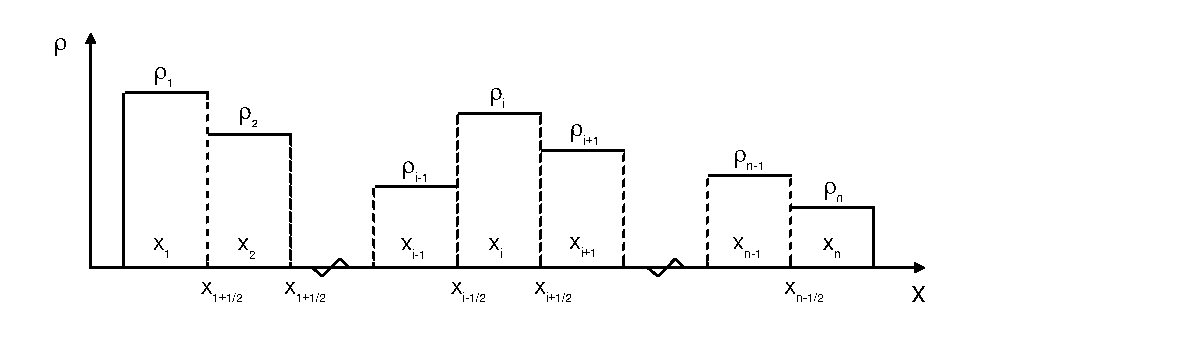
\includegraphics[trim=20 20 120 10,clip,width=\textwidth]{discretisation.pdf}
		\caption[Approach : 1D finite difference discretisation]{Discretisation of a 1D spatial domain for a single time. For $i\in\mathds{Z}$, $x_i$ represent the control volumes where single Godunov averaged solutions are stored, $\rho_i$. The cell interfaces are represented at locations $x_{i\pm1/2}$; as single solutions are stored in one cell, there are discontinuities at each cell interface location.}
		\label{fig:1d_discretisation}
	\end{figure}
	
\section{Compressible Flow Waves}
\label{sec:waves}

	Compressible dynamics numerical methods have been developed to allow flow variables to exhibit discontinuous derivatives in space, these variable jumps are due to the presence of flow waves. There are four types of compressible waves discussed here; normal shock, contact surface, rarefaction, and compression waves. When a region of high pressure and density is separated by a diaphragm from a region of low pressure and density\footnote{Such as the initial conditions for 1D shock tube and 2D explosion case.}, some of these waves occur. \\ \\
	Normal shock waves, such as the shock present on the upper surface of a transonic aerofoil, are normal to a surface. Contact surfaces propagate through a dynamic fluid as the discontinuous interface between two materials. Rarefaction waves represent gradual longitudinal expansion, propagating through the flow. Compression is the opposite of rarefaction, where a compression of characteristics move with the flow.
	
	
\section{Godunov-Type Methods}
\label{sec:Godunov}

	The Godunov method assumes piecewise constant solution profiles (see Figure \ref{fig:1d_discretisation}), with discontinuities along cell interfaces that induce many local Riemann problems \cite{Toro09}. Godunov's method improves on central-based schemes by having the capability to distinguish between compression and expansion fan waves \cite{Jayanti18}. Godunov \cite{Godunov59} suggested the following method for computing the interface flux approximations:
	\begin{itemize}
	\item[1.] Construct two \emph{local} Riemann problems over a data pairs $(\rho_{i-1}^n,\rho_{i}^n)$ and $(\rho_i^n,\rho_{i+1}^n)$,
	\item[2.] Average the two solutions over $[x_{i-1/2},x_{i+1/2}]$,
	\item[3.] Assign a value for $\rho_i^{n+1}$,
	\item[4.] Then the Godunov flux is approximated by
		      \begin{equation}
		      	\mathbf{F}_{i\pm1/2}=\mathbf{F}\left(\mathbf{U}_{i\pm1/2}\right). \nonumber
		      \end{equation}
	\end{itemize}
	The two Riemann problems are formulated locally (by scaling the variables as in Equation \ref{eq:local_scale}) with the equation $\rho_t+f(\rho)_x=0$, and each set of boundary conditions
	\begin{equation}
		(\rho_{i-1}^n,\rho_{i}^n) \, : \quad \rho(x,0)=
		\begin{cases}
			\rho_{i-1}^n, & if \quad x<0, \\
			\rho_i^n, & if \quad x>0,
		\end{cases}
		\nonumber
	\end{equation}
	\begin{equation}
		(\rho_i^n,\rho_{i+1}^n) \, : \quad \rho(x,0)=
		\begin{cases}
			\rho_i^n, & if \quad x<0, \\
			\rho_{i+1}^n, & if \quad x>0.
		\end{cases}
		\nonumber
	\end{equation}
	The cell averaging for $\rho_i^{n+1}$ is taken over the cell width, however with the locally formulated Riemann problems this is over $[-\Delta x/2,\Delta x/2]$, for the two Riemann problem solutions $\tilde \rho_{i-1/2}$ and $\tilde \rho_{i+1/2}$. The new solution is given by
	\begin{equation}
		\Delta x\cdot \rho_i^{n+1}=\int_{-\Delta x/2}^0\tilde \rho_{i-1/2}\mathrm{d}x +\int_0^{\Delta x/2}\tilde \rho_{i+1/2}\mathrm{d}x\label{eq:GodunovUpdate}
	\end{equation}
	Fluid dynamics problems are usually formulated as a combination of varying PDEs, solutions to which are highly sensitive to numerical methods \cite{Chung02}. Godunov schemes are useful when applied to hyperbolic systems, however have limitations for other types of PDEs. Elliptical problems have no real characteristic curves so flow variable derivatives are smooth with no discontinuities, hence the Godunov method and local Riemann problems are not useful \cite{Chung02}. The major disadvantage of using Godunov schemes with Riemann solvers for shock capturing flow is the extra computational cost over a second order scheme with artificial viscosity \cite{Woodward84}. Riemann solvers become complicated to implement if an equation of state cannot be represented with a gamma law. Analytical solutions of Riemann problems exist for the Euler equations however are computationally expensive, hence the Godunov local Riemann problems are solved using approximate methods shown in Section \ref{sec:RSFC}.	

\section{Approximate Riemann Solvers}
\label{sec:RSFC}

	The following methods for finding approximate solutions to local Riemann problems at each cell interface are presented for interest, only the Lax-Friedrichs, Rusanov, HLL and Murman-Roe solvers are included in the TFM program code, see Appendix \ref{code:main} lines [394-470]. As shown in Chapter \ref{ch:randd}, one of the flaws of this model is the ill defined Riemann solvers. An appropriate definition of parameters involved in the following methods is needed to yield a more realistic solution to the cell interfaces. This process in the simulation is known both as the approximate local Riemann problem solution and the calculation of numerical fluxes. These local problems are too computationally costly to apply exact Riemann solvers, hence approximate methods are used to cut this cost \cite{Laney98}.
	
\subsection{Rusanov and Lax-Friedrichs Flux}
\label{sec:RLF}

	The Rusanov \cite{Rusanov61} and Lax-Friedrichs \cite{Lax54} fluxes can both be written in the form
	\begin{equation}
		\mathbf{F}=\frac{1}{2}\left[\left(\mathbf{F}_L+\mathbf{F}_R\right)-S^+\left(\mathbf{U}_R-\mathbf{U}_L\right)\right], \label{eq:Rusanov}
	\end{equation}
	where the wave speed $S^+$ is calculated from local data in the Riemann problem, where both
	\begin{equation}
		S^+=\max\left(\left|f'\left(u_L\right)\right|,\left|f'\left(u_R\right)\right|\right),\label{eq:srus}
	\end{equation}
	\begin{equation}
		S^+=\frac{\Delta x}{\Delta t},\label{eq:slf}
	\end{equation}
	represent the maximum wave speed for the Rusanov (Equation \ref{eq:srus}) and Lax-Friedrichs (Equation \ref{eq:slf}) fluxes. These solvers can be found in Appendix \ref{code:main} lines [412-430], where the left and right state derivatives (Rusanov) are calculated from the chosen stream model. 
	
\subsection{Murman-Roe}
\label{sec:MR}

	The popular Roe solver defined for a scalar system is named the Murman-Roe solver \cite{Murman74}. Murman defines the wave velocity $a$ as the Rankine-Hugoniot velocity, 
	\begin{equation}
		a\left(\rho_L,\rho_R\right)=\frac{f_L-f_R}{\rho_L-\rho_R},
	\end{equation}
	and flux,
	\begin{equation}
		f\left(\rho_{L},\rho_{R}\right)=\frac{1}{2}\left(f_{L}+f_{R}\right)-\left|a\left(\rho_L,\rho_R\right)\right|\left(\rho_{R}-\rho_{L}\right),
	\end{equation} 
	if $\rho_L\neq\rho_R$.  However if $\rho_L=\rho_R$ then the velocity is defined as,
	\begin{equation}
		a\left(\rho_L,\rho_R\right)=f'_L=f'_R,
	\end{equation}
	and the flux depends on this velocity as follows,
	\begin{equation}
		f\left(\rho_{L},\rho_{R}\right)=
			\begin{cases}
				f_L, &\text{if}\quad a\left(\rho_L,\rho_R\right)>0,\\
				f_R, &\text{if}\quad a\left(\rho_L,\rho_R\right)\leq0.
			\end{cases}
	\end{equation}

\subsection{HLL}
\label{sec:HLL}

	Harten, Lax and van Leer \cite{HLL83} suggested a Riemann solver which assumes a wave formation of two waves, however this is incorrect for the Euler equations and only holds for two equation hyperbolic systems \cite{Toro09}. Hence the integral-form conservation equations are split over three regions, left and right states and a single \emph{star} region. Depending on the choice of left and right wave speed values, $S_L$ and $S_R$, the HLL flux is given by
	\begin{equation}
		\mathbf{F}=
		\begin{cases}
			\mathbf{F}_L, & if \quad 0\leq S_L, \\
			\mathbf{F}_M=\frac{S_R\mathbf{F}_L-S_L\mathbf{F}_R+S_LS_R\left(\mathbf{U}_R-\mathbf{U}_L\right)}{S_R-S_L}, & if \quad S_L\leq0\leq S_R,\\
			\mathbf{F}_R, & if \quad S_R\leq0.
		\end{cases}
		\nonumber
	\end{equation}
	As well as this formulation, Toro et al. \cite{Toro94} outline the problem with this Riemann solver. Namely the difficulty in finding reliable and simple estimates for the left and right wave speeds. Toro developed the HLL solver further, details of the HLLC Riemann solver are given in Appendix \ref{ap:HLLCriemann}. 
	
\subsection{Wave Speed Estimations}
	All previous Riemann solvers have depended on a set of parameters defining the behaviour of each Riemann solver, including the wave speed values of $S_L,\,S_R,\,S_*$. Davis \cite{Davis88} suggested a set of simple estimates for Riemann solvers in compressible gas dynamics where the quantity $a$ represents the local speed of sound. Toro showed that these estimates are however impractical for computations \cite{Toro09},
	\begin{equation}
		S_L=u_L-a_L, \quad S_R=u_R+a_R, \nonumber
	\end{equation}
	and
	\begin{equation}
		S_L=\min\left(u_L-a_L,u_R-a_R\right), \quad S_R=\max\left(u_L+a_L,u_R+a_R\right). \nonumber
	\end{equation}
	Davis \cite{Davis88} also uses the Roe-averaged eigenvalues
	\begin{equation}
		S_L=\tilde u-\tilde a, \quad and \quad S_R=\tilde u+\tilde a, \nonumber
	\end{equation}
	with Roe-averaged speeds denoted by $\sim$, which lead to a much more effective scheme. Davis also recognised how the Rusanov flux (Equation \ref{eq:Rusanov}) can be recovered from the HLL formulation by setting $S_L=-S^+$ and $S_R=S^+$ for some choice of $S^+$ mentioned in Section \ref{sec:RLF}. This aspect of the relationship between solving local Riemann problems in cell reconstruction in TFM is not equivalent to other fields such as gas dynamics, appropriate parameters to describe the local Riemann problems need to be established for the solvers described here to be most effective.
	
\section{Spatial Reconstruction}

	Prior to providing left and right states to a chosen Riemann solver to evaluate the numerical flux and proceed with the iteration, one can reconstruct the cell variable value in many ways. The most simple approach is named 1$^{st}$ order as the values provided for numerical flux calculations are in fact the cell average Godunov values themselves with no reconstruction applied. The next improvement is the 2$^{nd}$ order total variation diminishing scheme. At each cell interface (cell $i$, left $i-1/2$, right $i+1/2$), the left and right densities are 2$^{nd}$ order TVD reconstructed according to
	\begin{equation}
		\rho_L=\rho_i+\frac{\Delta_i}{2}, \quad and \quad \rho_R=\rho_{i+1}-\frac{\Delta_{i+1}}{2},\label{eq:tdv}
	\end{equation} 
	\begin{equation}
		\Delta_i=\mathrm{minmod}\left(\rho_i-\rho_{i-1},\rho_{i+1}-\rho_i\right), \nonumber
	\end{equation}
	\begin{equation}
		\mathrm{minmod}\left(x,y\right)=\frac{1}{2}\left(\mathrm{sign}\left(x\right)+\mathrm{sign}\left(y\right)\right)\min\left(\left|x\right|,\left|y\right|\right), \label{eq:minmod}
	\end{equation}
	where the slope limit $\Delta_i$ is calculated from the minmod limiter function.
	
\subsection{High Resolution Schemes}
\label{sec:HRS}
	
	High resolution numerical schemes are used when fluid problems involving shocks and discontinuities are of interest with high accuracy, high resolution methods reduce oscillations to provide monotone solutions \cite{Chung02}. Monotonicity preserving schemes are at most first order accurate according to Godunov's theory, where higher order schemes introduce oscillations around discontinuities \cite{Cockburn01}. Alternative to the uniform distribution over cells in Godunov's method, the MUSCL scheme which uses linear reconstructions of Godunov cell data. When accuracy greater than second order is required, WENO schemes provide higher accuracy. See Figure \ref{fig:high_res_schemes} for the comparison of a 1D problem solution using various discussed schemes. 
	\\ \\
	The first WENO scheme was proposed by Liu, Osher and Chan in 1994 \cite{Liu94}, a novel ENO method with a higher order reconstruction. Where the ENO method chooses the smoothest interpolating polynomial, the weighted scheme uses a convex combination of all polynomials with weights specifically chosen to improve on the accuracy of the ENO scheme. ENO schemes attempt higher order accuracy and to avoid oscillations at discontinuities \cite{Chung02}. WENO implementation can be either component-wise or characteristic wise, in terms of the cell reconstruction procedure. A review of reconstruction methods for ENO and WENO schemes are given in full detail in \cite{Shu97}. Component-wise applies scalar reconstruction procedures to each conserved vector component at each cell interface, then applies an exact or approximate Riemann solver to form the high resolution scheme. Characteristic-wise computes average state values, and the left and right Jacobian eigenvectors, then the eigenvectors are used to transform the cell variables to characteristic variables which are then reconstructed using WENO/ENO procedures. The component method is more simple to implement yet the characteristic method is more robust \cite{Shu97}. See Appendix \ref{ap:WENOreco} for the WENO algorithms used.
	\\ \\
	Proposed by Bram van Leer in 1979 \cite{vanLeer79} the MUSCL scheme was able to achieve second order accuracy and behaved at least an order of magnitude more efficient that Godunov schemes, equivalent of refining a mesh with factor two. Van Leer's MUSCL approximates the cell density distribution with polynomials of order $n\in\left\{2,3\right\}$, this alone would introduce large oscillations in the presence of shocks. To reduce oscillations and ensure the scheme is TVD, the slope limiter $\phi$ is applied at left and right states. TVD schemes reduce to first order at local extrema, and are as high order as the general scheme in smooth regions. The 2nd order MUSCL scheme approximates the cell density distribution with a linear slope, whereas the 3rd order scheme approximates with a parabolic slope from a second order interpolation. Oscillations may appear in solutions with large flow variable gradients due to a numerical procedure with no artificial dissipation \cite{Tu18}, the latter will reduce flow to a monotone solution however is inaccurate. To keep monotonicity yet eliminate the need for artificial dissipation, flux gradient limiters are used. Barth and Jesperson \cite{Barth89} suggest a slope limiter, $\phi_i$, which limits the gradient in the reconstruction
	\begin{equation}
		R_i\left(x_j-x_i\right)=\rho_i+\phi_i\nabla \rho_i\left(x_j-x_i\right), \quad with \quad \phi\in[0,1]. \nonumber
	\end{equation}
	Mathematical descriptions of two limiters have been summarised from Michalak and Ollivier-Gooch \cite{Gooch08}, where reconstruction is described with the need of gradient limiters and a useful algorithm for the Barth and Jespersen limiter is presented which can be developed into Venkatakrishnan's limiter. See Appendix \ref{ap:MUSCLreco} for the MUSCL algorithms used. 
	\begin{figure}
    		\centering
        		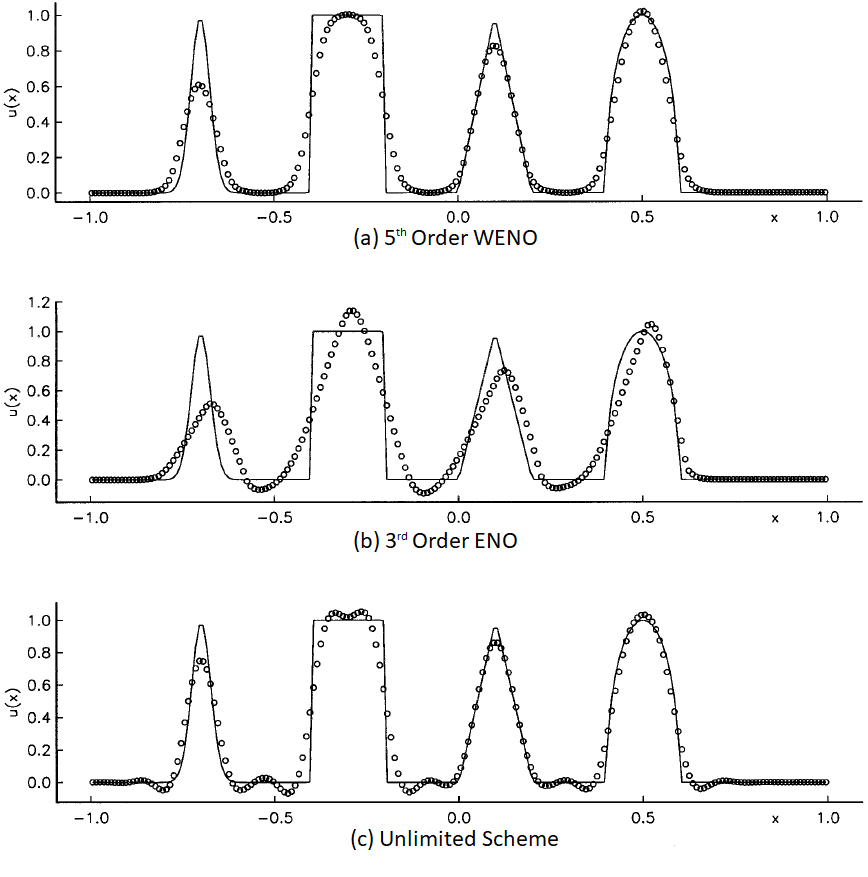
\includegraphics[trim=0 0 0 0,clip,width=0.6\textwidth]{high_res.png}
		\caption[Approach : Comparison of high resolution schemes]{1D advection equation results from Suresh and Huynh \cite{Suresh97}. The unlimited scheme (c) is not high resolution, hence oscillations appear in the solution in regions of high gradient $\partial \rho/\partial x$ discontinuities. Using the smoothest polynomial reconstruction in the 3$^{\mathrm{rd}}$-Order ENO scheme (b) finds a monotone improvement from (c). Using a specific weighted average of polynomials, the 5$^{\mathrm{rd}}$-Order WENO (a) scheme has improved accuracy by choosing appropriate polynomials not just the smoothest one, as in ENO (b). }
		\label{fig:high_res_schemes}
	\end{figure}
	
\newpage
\section{Limitations of Finite Difference Schemes}

	Finite difference is the approach of describing derivatives by finite discrete values. Chung presents many FDMs and evaluates their performance \cite{Chung02}. FDM can only be used on structured grids\footnote{More generally FDM can also be used on \emph{transformations} of orthogonal structured grids}. Hyperbolic PDEs are used to model wave propagation; FDM are limited by strict stability criterion restricting spatial and time step sizes, with are due to bounding the dissipative error growth. All \emph{implicit} FDM schemes however are unconditionally unstable. Low-resolution schemes are inaccurate at discontinuities, either over or underestimating with oscillations. Improving the order of accuracy in FDM requires more initial data. Extra solving tools are required to improve the accuracy, including high resolution methods, Riemann solvers and reconstruction procedures with gradient limiters. The higher resolution group of TDV methods are considered higher order but the accuracy is not uniform, TDV schemes may range from first to second order accuracy in different solution regions. Solving systems of hyperbolic PDEs includes the calculations of Jacobians which are computationally inconvenient. 
	
\section{Time-Update Scheme}
\label{sec:timeupdatescheme}

	The single step discretisation update given in Equation \ref{eq:GodunovUpdate} will not allow some of the higher resolution schemes to exhibit their advantages over lower resolution methods. A commonly used time-update scheme is the classical 4$^{th}$ order Runge-Kutta process. First proposed by Runge \cite{Runge1895} and further developed or finalised into a family of methods by Kutta \cite{Kutta1901}, used by many in a wide field of study the modern Runge-Kutta framework provides a strong foundation for building a sophisticated time update scheme. The classical fourth order update is used in this TFM program, and can be found in lines [552-584] of the code in Appendix \ref{code:main}. This method uses an accumulative weighted average of four different updates, $RK_i$,  around the current time step. The updated density value is given by
	\begin{equation}
		\rho^{(n+1)}=\rho^{(n)}+\frac{dt}{6}\left(RK_1+2RK_2+2RK_3+RK_4\right),
	\end{equation}
	where the intermediate updates $RK_i$ are given by,
	\begin{align}
		RK_1&=f\left(t^{(n)},\rho^{(n)}\right),\\
		RK_2&=f\left(t^{(n+1/2)},\rho^{(n)}+\frac{RK_1}{2}\right),\\
		RK_3&=f\left(t^{(n+1/2)},\rho^{(n)}+\frac{RK_2}{2}\right),\\
		RK_4&=f\left(t^{(n+1)},\rho^{(n)}+RK_3\right).
	\end{align}
	This framework can be extended to adaptive step size based on two approximation errors, larger stability in implicit Runge-Kutta update methods.

\section{Probabilistic Network Model}
\label{sec:networkmodel}

	Previous studies \cite{Bretti07},\cite{ShiGuo16} of the fluid dynamics model application to traffic flow problems on networks provide a clear and useful mathematical description. These studies both use a traffic distribution matrix to describe the amount of flow distributed to any outgoing roads of a junction, from the incoming roads. This links the macroscopic continuum model together in a series of problems for each road segment defined by the network of interest. The macroscopic LWR model is derived by the conservation of traffic from each cell of a road segment, hence the conservation of traffic at junctions is equally as important. This junction conservation can be written as the Rankine-Hugoniot condition,
	\begin{equation}
		\sum_{i}f(\rho_i)=\sum_{j}f(\rho_j),\quad i\in\{1,\hdots,n\}, \quad j\in\{n+1,\hdots,n+m\}
	\end{equation}
	for the general junction with $n$ incoming roads, $m$ outgoing roads, and where $\rho_i$ and $\rho_j$ respectively represent the densities at the end of incoming roads and start of outgoing roads. The traffic distribution matrix $A=\left[a_{i,j}\right]$ has probability-like\footnote{Probabilities have $0<p<1$ and $\sum p=1$.} elements, satisfying the condition $\forall i$,
	\begin{equation}
		\sum_{j}a_{i,j}=1,
	\end{equation}
	as all flow leaving road $i$ must be distributed to outgoing roads. These definitions and properties are sufficient and consistent over \cite{Bretti07} and \cite{ShiGuo16}, with implementation given in \cite{Gcostese}, such that this approach can be applied to the traffic model listed in the junction solver of the code \emph{main.py} in Appendix \ref{code:main}  lines [326-374].
	
	\createblankpage
	
	\chapter{Program Development}
\label{ch:development}
\graphicspath{{image_directory/development/}}

\section{Developing Tools}

	The Python code was developed entirely in the PyCharm IDE \cite{PyCharm}, this tool allows a user to activate the GitHub version control functions and view the history log from within the editor. Python was chosen as the developing language for this tool due to its compatibility and cross platform benefits, a wide range of functionality can be achieved by importing specific modules. PyCharm allows the importing of many modules from within the editor itself. While developing it can be useful to have a terminal window and Python console at hand, both of which are integrated into PyCharm. As well as providing functional assistance the IDE provides developing tips while coding, PyCharm will suggest syntax choices for automatic fill when using special functions from modules or keywords. Keywords are easy to spot as PyCharm has a colour style (which can be change to many colour schemes) that allows numbers, function definitions, keywords and comments to be identified quickly and easily. The TFM tool developed here uses many different functions, while defining functions it is important to consider the scope of variable names used in the rest of the program, PyCharm will identify a conflicting variable name from within a function as to avoid scope error. See Figure \ref{fig:dev:pycharm} for the user interface from within the PyCharm IDE. 
	\\ \\
	All the code used to simulate traffic flow for results in Chapter \ref{ch:randd} are present on the TFM$\_$Thesis GitHub repository \cite{AndrewDixonGitHub}, available at \href{https://github.com/adj97/TFM_Thesis}{github.com/adj97/TFM$\_$Thesis}, see Figure \ref{fig:dev:github} for the homepage interface. GitHub is an opensource cloud storage system for program code of any sort. Not only are the current files stored, but a detailed history of every change to the system is noted. This is incredibly useful for adding extra features, where an entire copy of code is made and then developed on a new \emph{branch}, the new feature can then be merged back to the original copy once it has been tested, or alternatively revert back to the original. GitHub is also a useful community of developers, the Facebook of coding, if public then your repository can be viewed, reviewed, tested, cloned by any GitHub user. 

	\begin{figure}
        		\begin{minipage}{0.48\textwidth}
            		\centering
            		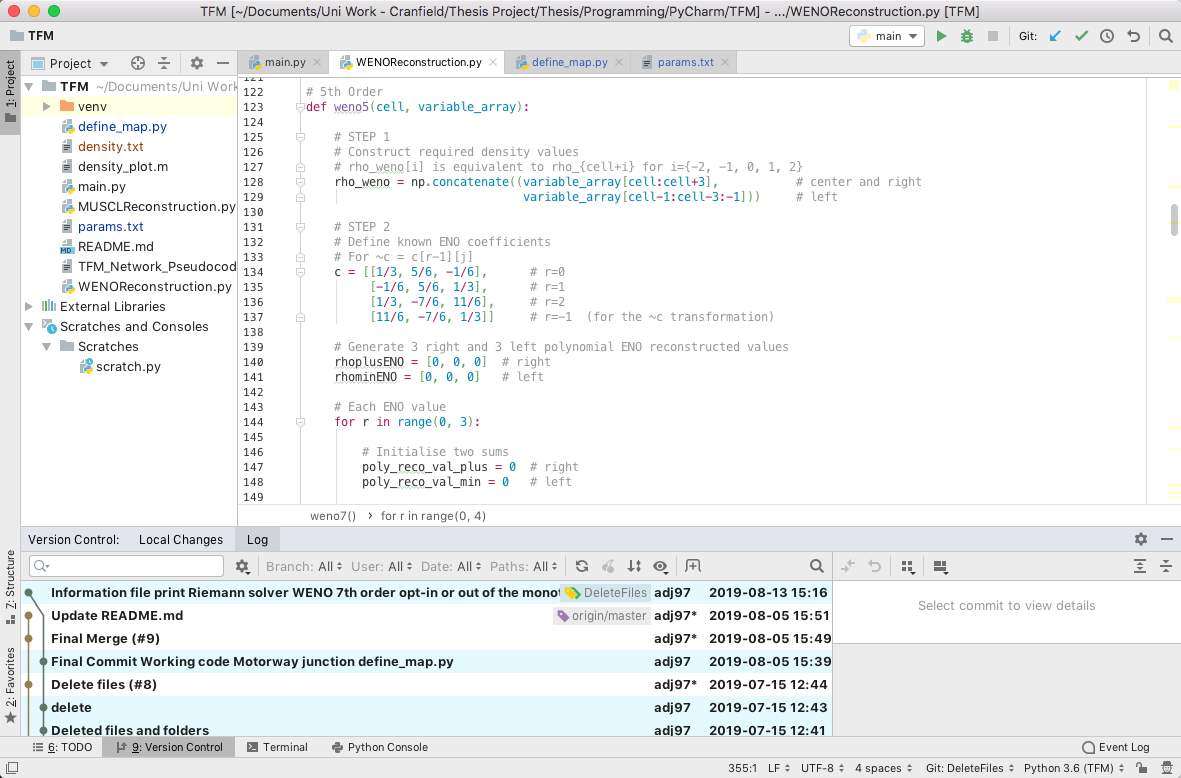
\includegraphics[trim=0 0 0 0,clip,width=\textwidth]{PyCharm.png}
            		\caption[Development : PyCharm IDE]{The multi-window GUI of the Pycharm IDE, the lower bar shows the version control log, left is the local file directory, and main window for the code editor with files open in different tabs.}
            		\label{fig:dev:pycharm}
        		\end{minipage}
        		\hfill
        		\begin{minipage}{0.48\textwidth}
            		\centering
            		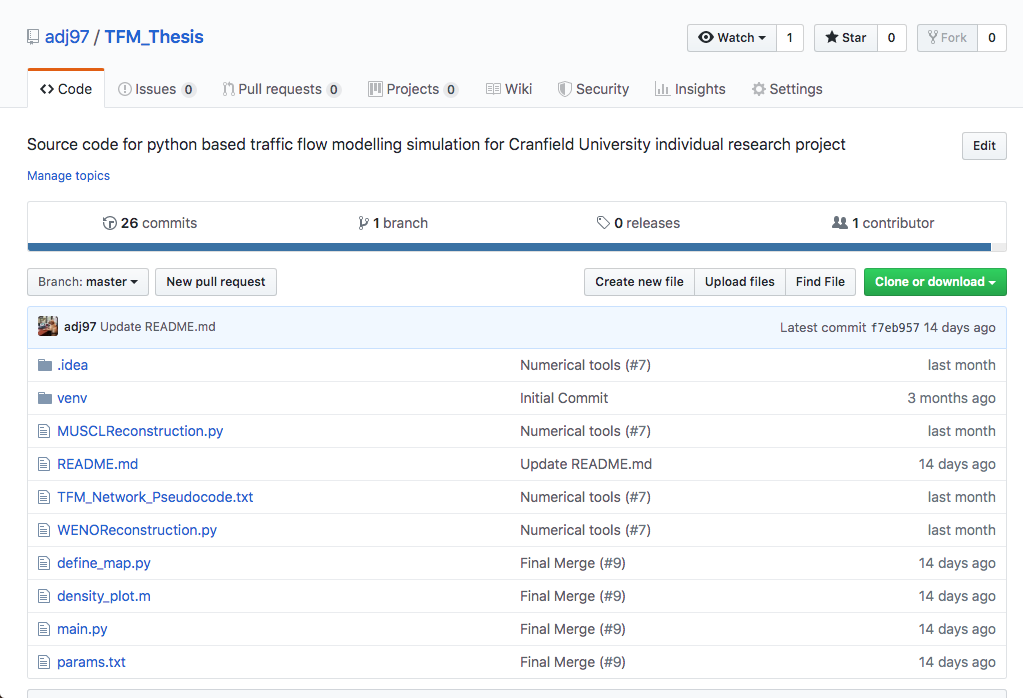
\includegraphics[trim=0 0 0 0,clip,width=0.97\textwidth]{GitHub.png}
            		\caption[Development : GitHub version control]{The TFM$\_$Thesis repository homepage, showing committed files and information on history of version control. This page links to all other features; issues, project management and all working branches.}
            		\label{fig:dev:github}
        		\end{minipage}
	\end{figure}

\section{Non-Numerical Features}

	The complex numerical procedure presented in \emph{main.py} (Appendix \ref{code:main}) is complemented by many non-numerical tools that improve ease of use, and provide extra information to the user. The following give a brief explanation to some of these features,
	\begin{itemize}
		\item Error checks and print statement - Once the program has read in the network and junction$\_$info dictionaries from \emph{define$\_$map.py}, and the parameters from \emph{params.txt}, many aspects of this input is checked for any non-compatible entries. The error types can be found in lines [55-60] of \emph{main.py} in Appendix \ref{code:main}. If any such errors are found then a breakdown of error messages and how many have occurred are printed before the program exits allowing the user to re-input information and try again. 
		\item Internal data structures - There are a wide number of arrays and data objects that have small and large features in the overall solver, listed are the main objects with a small description
		\begin{itemize}
			\item Dictionaries - Small information structures are useful to store in dictionaries as each entry will have a key tag that can be used to give meaningful names to objects.
			\item JSON file - The parameter text file is written in JavaScript Object Notation (JSON), this allows for quick and simple definition of the parameter values after being read in to the main program.
			\item Local flows - This is the output of the junction solver, which assigns each in/out road at a junction a flow value.
			\item Global flows - The local flows array feeds into this global flows array which acts every time step to define each road's supply and demand value to be used as boundary conditions in the iterated solution. 
			\item Source/Sink lists - A straight forward vector-type list of numbers defines both the road indexes of source and sink roads in two separate arrays. This is used to loop through and test if a road is a source/sink.
			\item Rho - The density solution is stored in this array, the whole network is can be stored road-by-road back to back for every cell for every road.
			\item Supply/Demand in junction solver - For the junction solver, this array provides the flow values at the end of in-roads and start of out-roads.
			\item Ghost densities - Prior to calculating the reconstructions, some high resolution schemes require values outside of the solution domain. This ghost array provides these values with symmetrical conditions at domain boundaries.
			\item Reconstructed - Looping through each cell, this array has two columns that are used to store the left and right reconstructed states for each cell.
			\item Cell fluxes - Reading from the reconstructed array (above), the chosen Riemann solver will compute from the two values of reconstruction at a cell interface. This array stores the Riemann problem approximate solution at the right hand side cell interface for each cell.
			\item Runge-Kutta arrays - Four separate lists of the density solution are stored, each represent the value after each Runge-Kutta iteration.
		\end{itemize}
		\item Function : get-start-end - This function is crucial to the data structure approach of storing the whole network solution in a single array. The function will return two indexes for the start and the end of the prescribed road of interest index.
		\item Loop progress bar - Giving the user more information on the progress of a simulation, this feature, shown in Figure \ref{fig:dev:progressbar}, is taken from \cite{TQDM} and is available at \href{https://github.com/tqdm/tqdm}{github.com/tqdm/tqdm}.
		\item Timing Segments - To provide information about the time spent in certain areas of the code, timing trackers are placed and results are printed in simulation output info (next in this list), these results are shown in Section \ref{sec:randd:timeanalysis}.
		\item Output information - Meaningful console (Appendix \ref{txt:info:console}) and information text file (Appendix \ref{txt:info:file}) print statements are provided if requested. The saved text file is placed in new created folder (named as the date and time) in the main working directory, which also includes the final density solution. This allows many simulations to be completed while not losing information on which parameters have been used to generate the solution. Included in the information file is a line count for all code contributing to the program, and a measure of the size of the final density solution output.
	\end{itemize}
	
	\begin{figure}
    		\centering
        		\fbox{
\includegraphics[trim=0 0 0 0,clip,width=0.7\textwidth]{progressbar.pdf}}
		\caption[Development : Simulation progress bar]{The information shown on the progress bar is (left to right): overall loop percentage complete, moving partial progress bar, loops completed/total number of loops, total time elapsed, estimated time remaining, loop speed in iterations per second.}
		\label{fig:dev:progressbar}
	\end{figure}
	
\section{File Structure}

	It is practical to arrange code in an organised manner, this includes splitting large code chunks into separate files and ordering each file to input or apply when necessary. The run procedure for this TFM program is to execute the \emph{main.py} code, this will call three other Python files, and read in a single parameter text file. Firstly the definition of the road network of interest is entirely contained within \emph{define$\_$map.py}, this means there is no need to alter the code in \emph{main.py} before use. The other two Python files that are used contain the MUSCL and WENO reconstruction procedures, presented as functions that take in the density array and a cell index which identifies the cell to reconstruct. These, like \emph{main.py}, need no code changes before running a simulation. Once a simulation is complete and the \emph{density.txt} output file is saved, any MATLAB postprocessing scripts can be used to analyse the results, for example splitting the array into a density profile for each road and plotting according to the road network. 
	
\section{Simulation Procedure}

\subsection{Pre-Processing}

	Prior to executing the simulation code, one needs to plan the study. The input in \emph{define$\_$map.py} requires lots of information about the roads and the junction links. It is useful to sketch a simplified diagram such as in Figure \ref{fig:networkdiagram}, which includes the direction for each road, identifies sources and sinks, and which gives indexes to each road and junction. Other information required for input are the each road length, maximum speed, and jam density. This diagram will help establish the road indexes, and allows the junctions to be identified by the road indexes of in and out roads. The only remaining aspect of network definition are each junction's individual TDM, the elements of which have constraints (See Section \ref{sec:networkmodel}) but can be estimated with rational.
	
	\begin{figure}
    		\centering
        		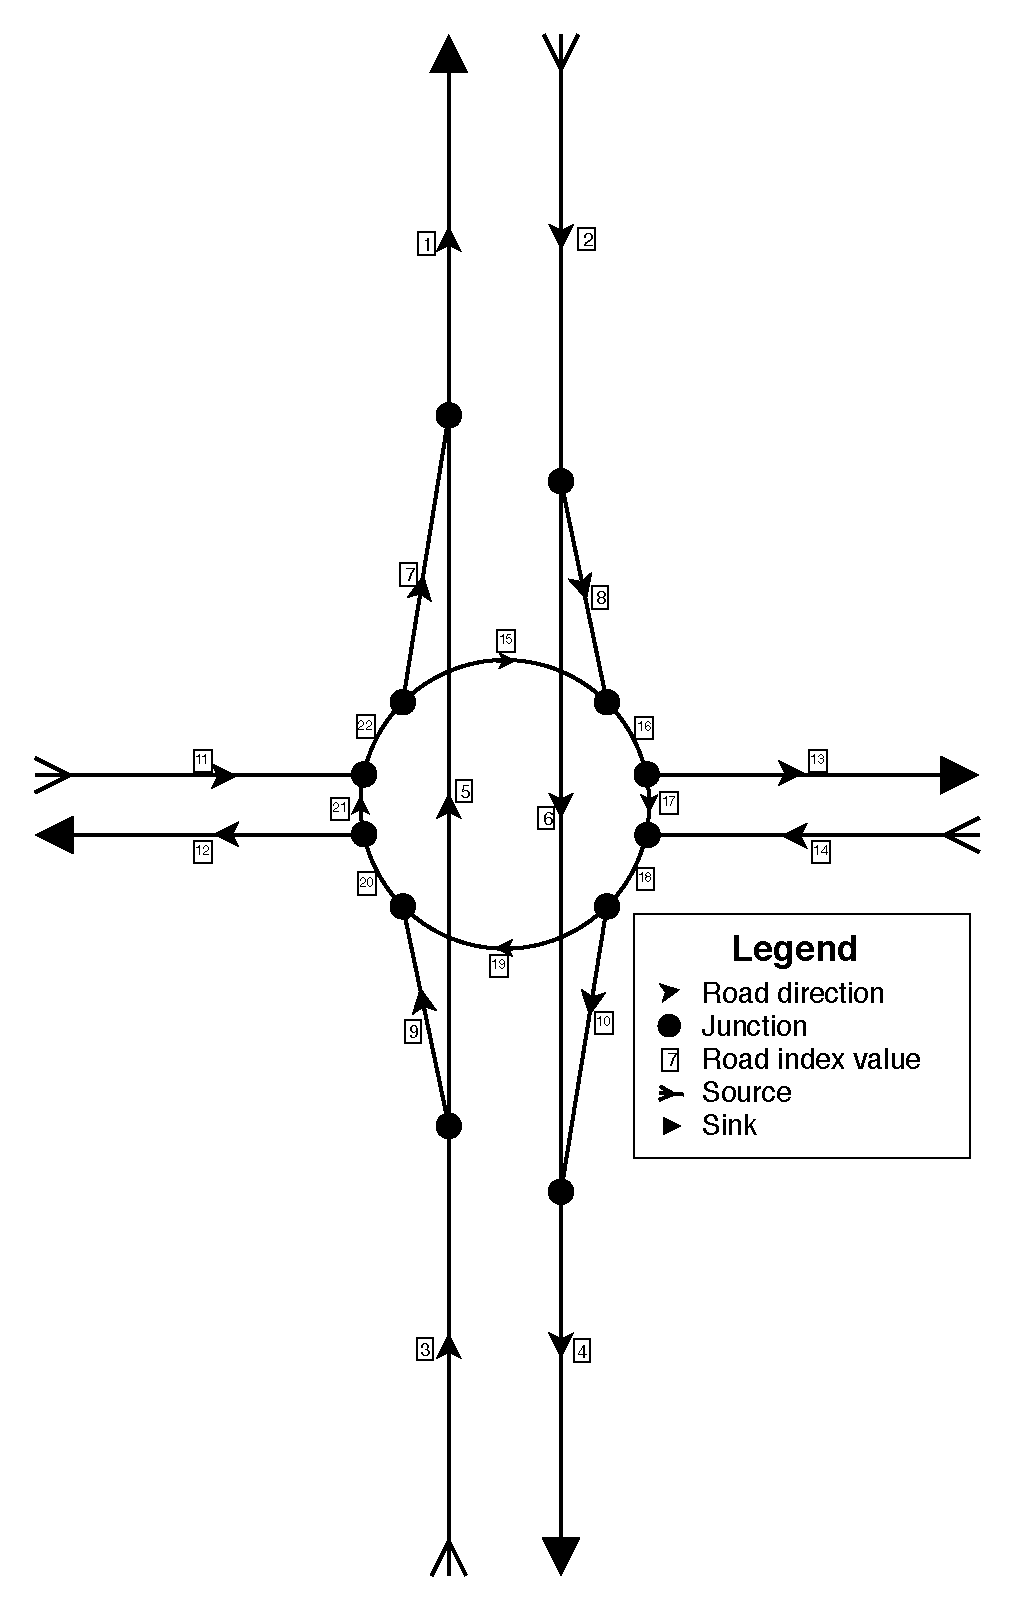
\includegraphics[trim=0 0 0 0,clip,width=0.9\textwidth]{MapDiagram.pdf}
		\caption[Development : Network map diagram]{A diagram theme for planning the definition of a road network into \emph{define$\_$map.py}, this diagram represents the Wakefield M1 junction 40 network presented in Section \ref{sec:randd:M1J40}.}
		\label{fig:networkdiagram}
	\end{figure}

\subsection{Code Algorithm}

	Once the previous steps have been carried out to define the road network of choice, the code in \emph{main.py} can be executed and the procedure outlined in Figure \ref{fig:simflowchart} will be carried out resulting in a solution profile and information file being saved to a local results folder.

	\begin{figure}
    		\centering
        		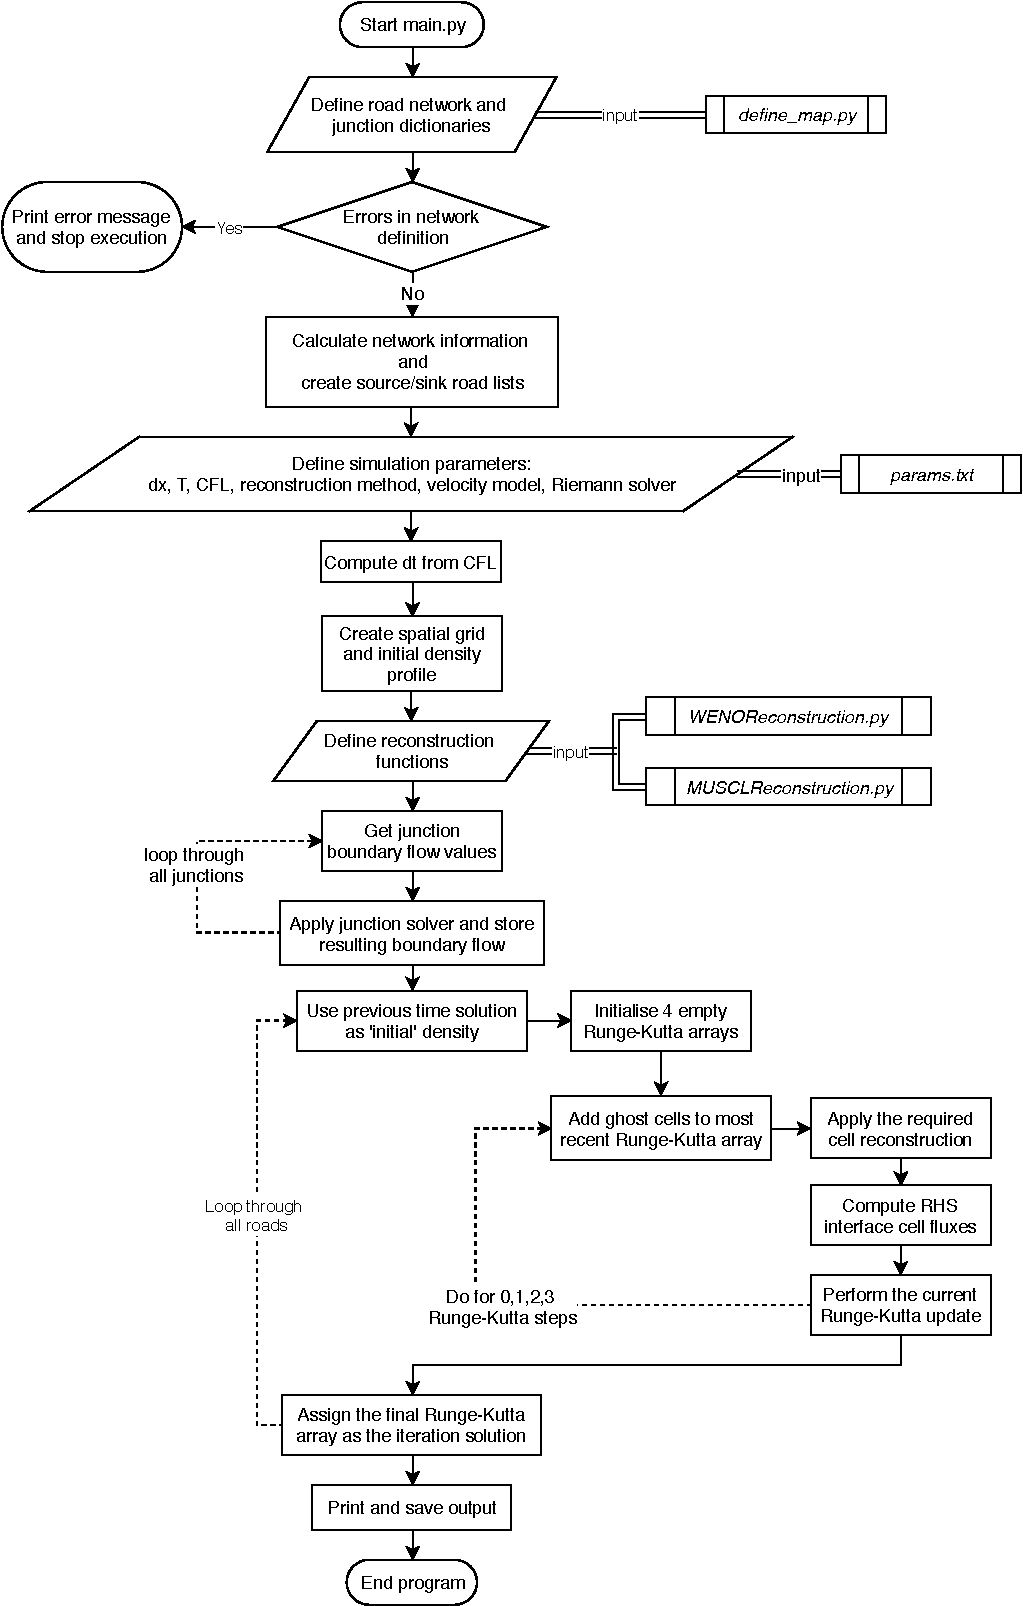
\includegraphics[trim=0 0 0 0,clip,width=\textwidth]{FlowChart.pdf}
		\caption[Development : Simulation process flowchart]{Simulation process key steps flowchart.}
		\label{fig:simflowchart}
	\end{figure}

\subsection{Postprocessing}

	The resulting \emph{density.txt} file is difficult to interpret raw; after being read in by a MATLAB script, this array can be split into many smaller objects containing the density for all time steps on a single road section each. Some example MATLAB postprocessing scripts are given in Appendix \ref{code:MATLABpostprocessing}, these can be used with no change to recreate some results of Chapter \ref{ch:randd}, or can be used as a template to develop a new script for a new road section. 
	
	\createblankpage
	
	\chapter{Results and Discussion}
\label{ch:randd}
\graphicspath{{image_directory/resultsanddiscussion/}}

	The following results are organised as the following: simple theoretical road networks used to test numerical features, road sections from two real-world locations showing the application of this model to real situations, and an analysis of various simulation times. 
	
\section{Simple Road Tests}

	To begin using the model, the most simple road networks are to be tested. Is it useful to test over-simplified and somewhat unrealistic networks to show the working features of the probabilistic network model and some simple features such as the source and sink roads in action. Here a simple single road and a network, proposed by Bretti, Natalini, and Piccoli \cite{Bretti07}, known as the traffic circle resembling a common roundabout.
	
\subsection{Single Road Segment}
\label{randd:singleroad}

	The most simple network tested is a straight road with no junctions, made up of a single road segment that is both a source and a sink. The junction solver is not called as there are no defined junctions, hence this test can be executed very quickly due to the simple simulation process. 
	\\ \\ 
	This simple network is useful to expose individual features of the solver, such as the higher order WENO reconstruction methods. As described in Section \ref{sec:HRS} and given explicitly in Appendix \ref{ap:WENOreco}, the 5$^{th}$ and 7$^{th}$ order schemes are available as reconstruction methods. The 7$^{th}$ order method is equivalent by process to the 5$^{th}$ and 3$^{rd}$, with the addition of steps to preserve the monotonic bounds of each cell reconstruction \cite{BalsaraShu00},\cite{Suresh97}. Figure \ref{fig:randd:single:7thOrder} shows the 7$^{th}$ order density profile solution for the single road with 5$^{th}$ order as a reference. The yellow line shows the density profile for the unbounded-7$^{th}$ order WENO scheme. The solution following the 10$^{th}$ time step becomes \emph{numerically} unbounded for the unbounded-7$^{th}$ order WENO scheme. This shows that the procedure presented in Appendix \ref{ap:WENOreco}, for the general $(2k-1)^{th}$ scheme cannot be extended to $k\ge4$ without extra methodology applied such as the monotonicity preserving bounds \cite{BalsaraShu00}. This figure also highlights the advantage of the 7$^{th}$ order scheme over the 5$^{th}$, in terms of capturing density jumps to a higher accuracy. The 5$^{th}$ order scheme actually predicts a jump in density earlier than the main density drop, a high density clustering of fast moving cars at the front of the stream. This is unrealistic, and predicted better by the 7$^{th}$ order scheme.

	\begin{figure}
    		\centering
        		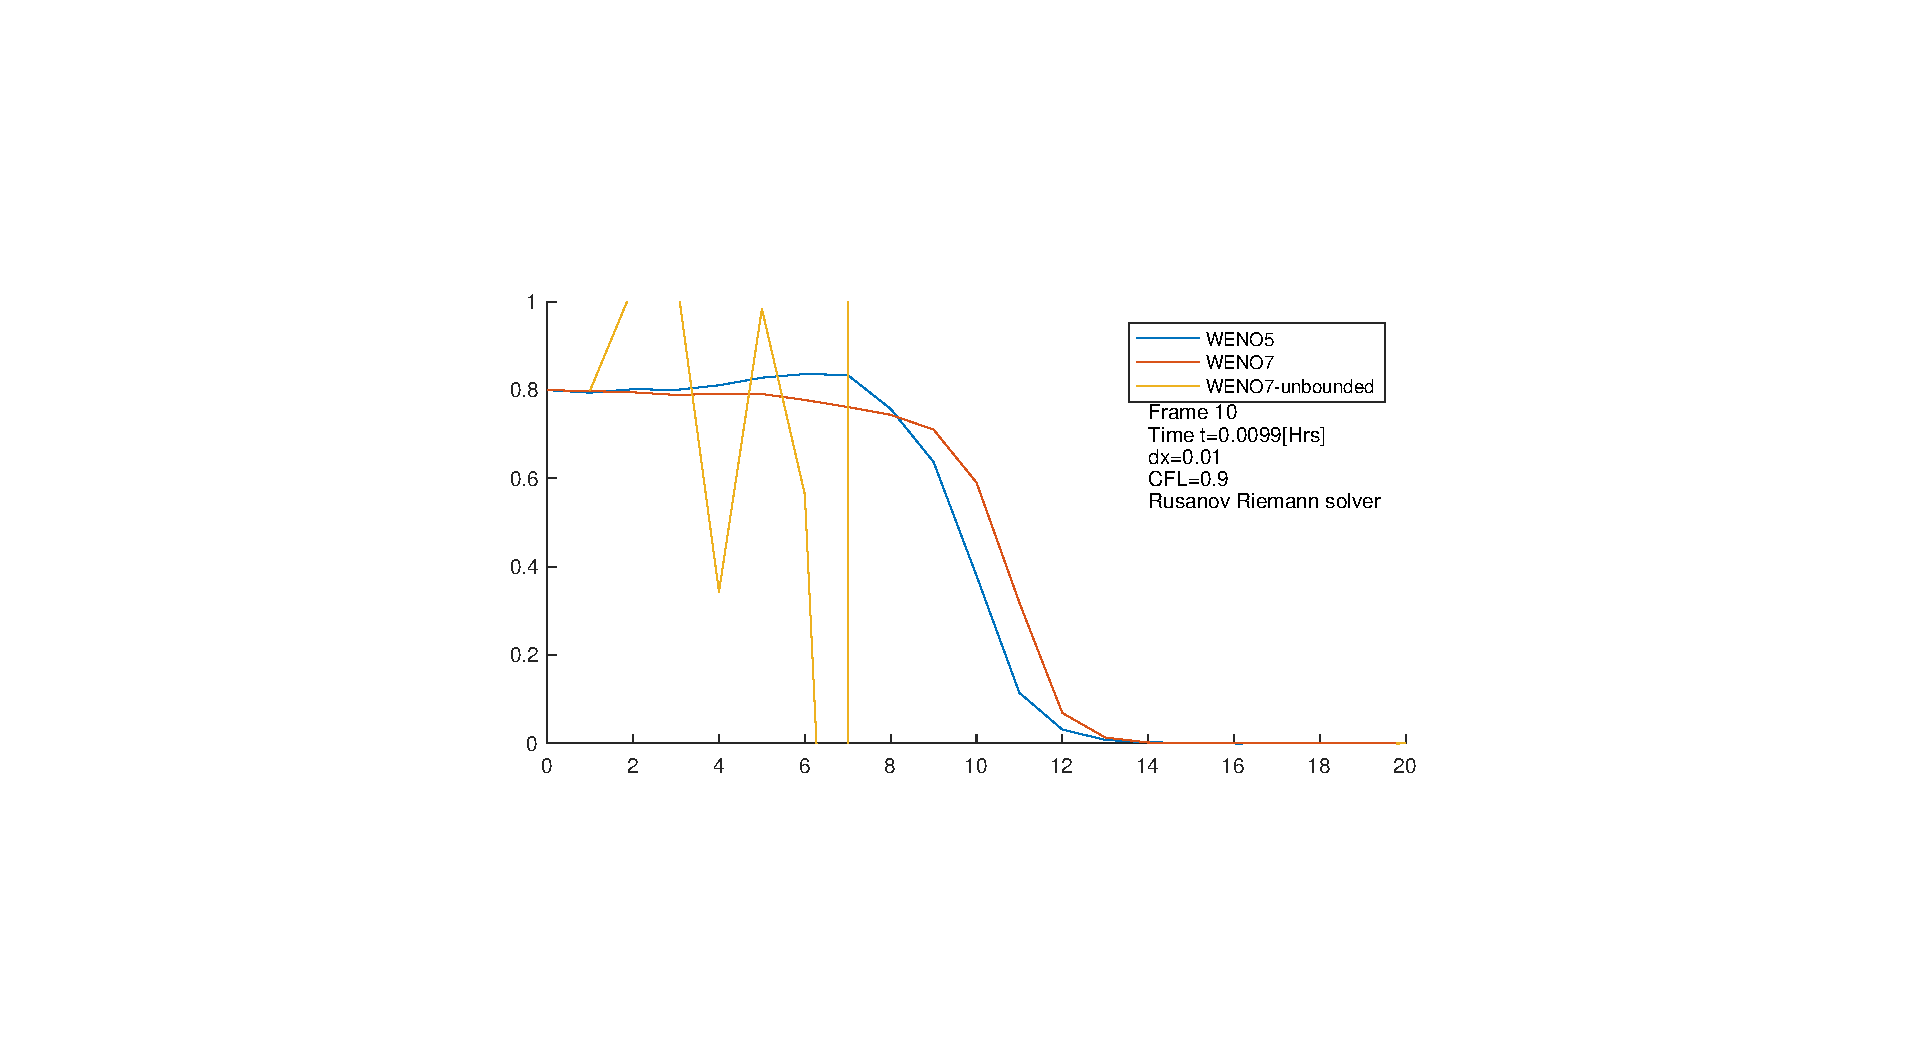
\includegraphics[trim=240 130 230 130,clip,width=0.7\textwidth]{SingleRoad_W7.pdf}
		\caption[Single Road : 7th order WENO]{The scheme used for 5th and 3rd order WENO reconstruction cannot be extended to 7$^{th}$ order without monotonic bounding applied. The unbounded solution is highly modulated, and becomes numerically unbounded after 10 time steps.}
		\label{fig:randd:single:7thOrder}
	\end{figure}

\subsection{Traffic Circles}
\label{randd:trafficcircles}

	The following simulations have reproduced the traffic-circles network and parameters from \cite{Bretti07}, with 8 roads joined by 4 junctions (as shown in Figure 9 of \cite{Bretti07}). Unless otherwise stated in the figure legend, the simulation settings for the results and following discussion are d$x=0.01$, $CFL=0.9$, $2^{nd}$ order reconstruction and Lax-Friedrichs Riemann solver. The defined inlet density from the left and right are 0.25 and 0.4 respectively, this feeds into the four central roads which can be shown by the jump in density along the four internal roads and top and bottom outlet roads, shown in all Figures \ref{fig:randd:traffic_circles_reco}, \ref{fig:randd:traffic_circles_riemann}, \ref{fig:randd:traffic_circles_dx}. 
	\\ \\
	It is expected that high order spatial reconstruction results in a more accurate prediction of jumps in traffic density, however  such simulation parameters as in Figure \ref{fig:randd:traffic_circles_reco}, there is no obvious advantage of the 3$^{rd}$ order WENO over 2$^{nd}$ order TVD reconstruction. The parameter $q_1=0.5$ describes equal flow joining and leaving the traffic circle at available junctions. A result of this some density will always remain in the central roads and the density profile will become smoother where the effect of spatial reconstruction is not as significant.
	\\ \\
	One major fault of the model concerning the numerical flux calculation is the definition of certain parameters used in calculations from Section \ref{sec:RSFC}. This is concluded from Figure \ref{fig:randd:traffic_circles_riemann} where the Rusanov, Murman-Roe and HLL solvers all appear to give an identical solution. The Lax-Friedrichs solution differs from the other solvers but in a less accurate manner in terms of shock resolution.
	\\ \\ 
	Another highly influential parameter in the resolution of density jumps is the spatial resolution $dx$, of which each road segment is split into cells of this size where the density profile is resolved. Figure \ref{fig:randd:traffic_circles_dx} gives another solution to the traffic circle network, with the values of $dx$ for each grid given in the caption. As expected the coarser resolution smooths out density jumps, whereas finer will capture a stronger shock, which is clear from this figure. The coarse and fine simulations give smooth density profiles in comparison to the medium solution which gives a slightly more oscillatory jump. 
	\\ \\
	Another aspect of the flow modelling that is analysed through the traffic circles network is the MUSCL reconstruction slope limiters, discussed in Section \ref{sec:HRS} and given in Appendix \ref{ap:MUSCLreco}. All of the 15 listed slope limiters are applied and solutions shown in Figure \ref{fig:randd:traffic_circles:limiters}, where the top row and bottom row respectively represent limiters applied to the 2$^{nd}$ and 3$^{rd}$ order MUSCL reconstructions. It is immediately clear that the 3$^{rd}$ order MUSCL reconstructed solutions are more oscillatory with all limiters. Of the 2$^{nd}$ order reconstructed solutions, the smoothest profiles arise from the Monotonised Central, UMIST and VanLeer limiters. The VanAlbada2 limiter is numerically unstable for both MUSCL schemes, the solution becomes so oscillatory that after sufficient time steps it is numerically unbounded. This may arise as a result of the violation of Sweby's TVD region \cite{Sweby84} for slope limiters, see Appendix Figure \ref{fig:app:slopelims}.

	\begin{figure}
    		\centering
        		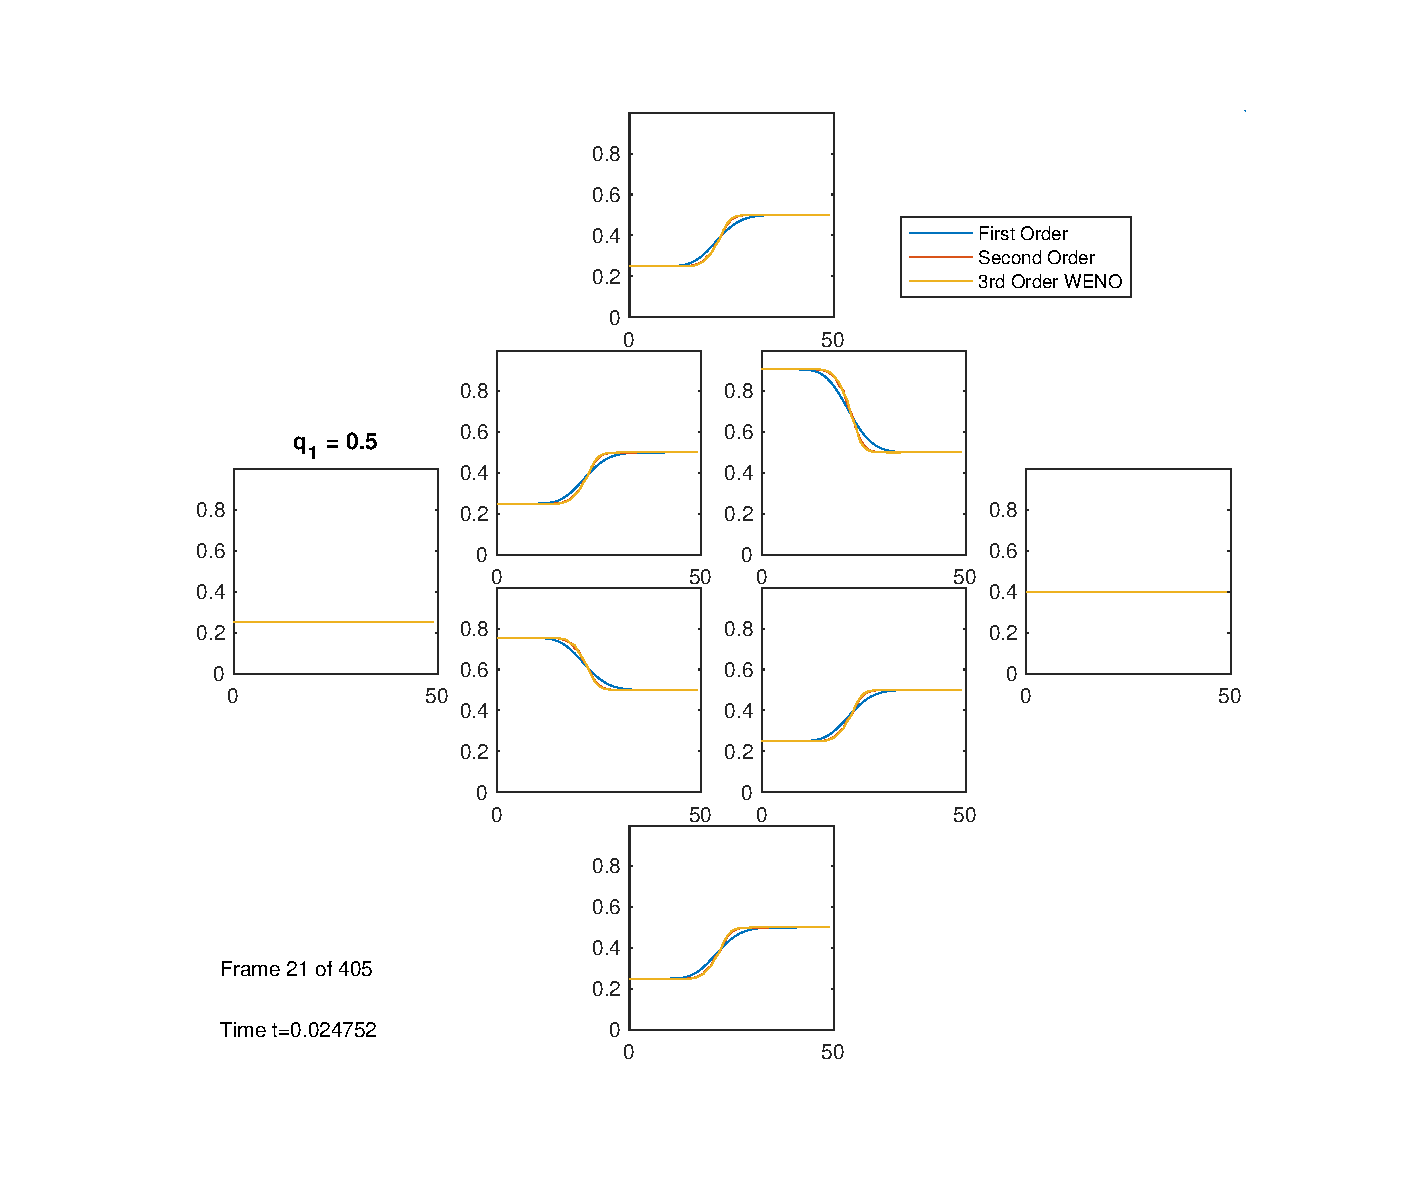
\includegraphics[trim=80 50 80 50,clip,width=0.78\textwidth]{trafficCircles1.pdf}
		\caption[Traffic Circles : Reconstruction methods]{Spatial reconstruction influence, lower order reconstruction smooths out local discontinuities.}
		\label{fig:randd:traffic_circles_reco}
	\end{figure}
	\begin{figure}
    		\centering
        		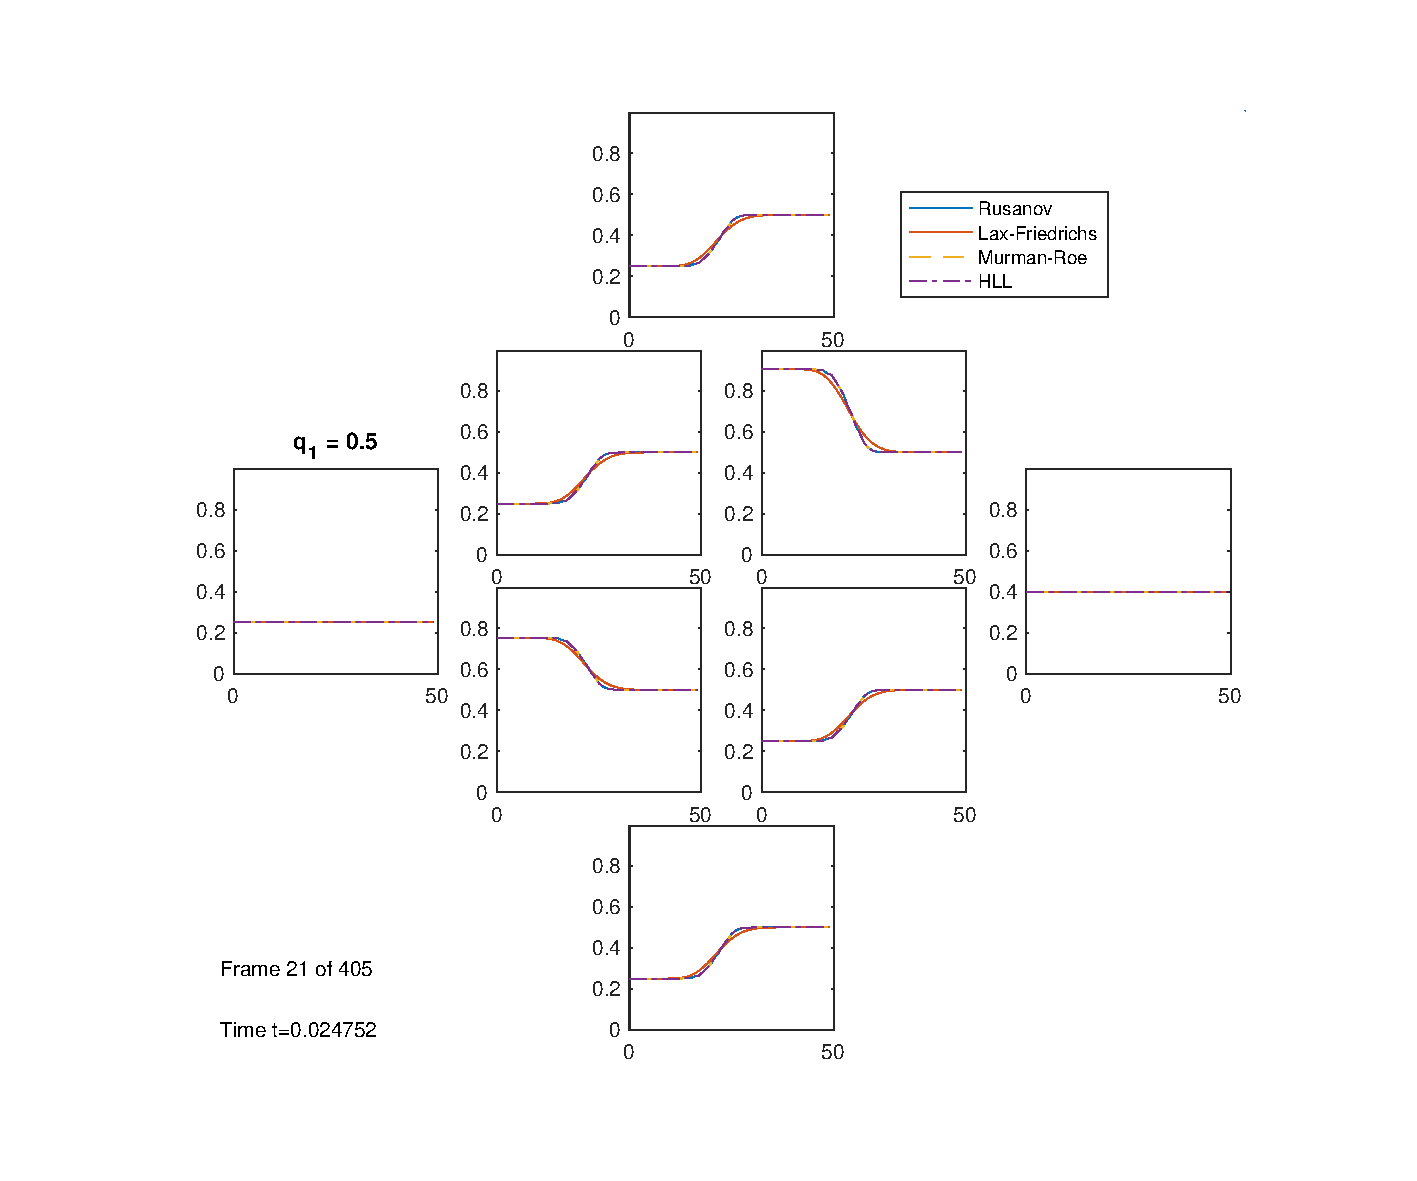
\includegraphics[trim=80 50 80 50,clip,width=0.75\textwidth]{trafficCircles2.pdf}
		\caption[Traffic Circles : Riemann solvers]{Varying the Riemann problem solution method, showing the equivalence of Rusanov, HLL and Murman-Roe.}
		\label{fig:randd:traffic_circles_riemann}
	\end{figure}
	\begin{figure}
    		\centering
        		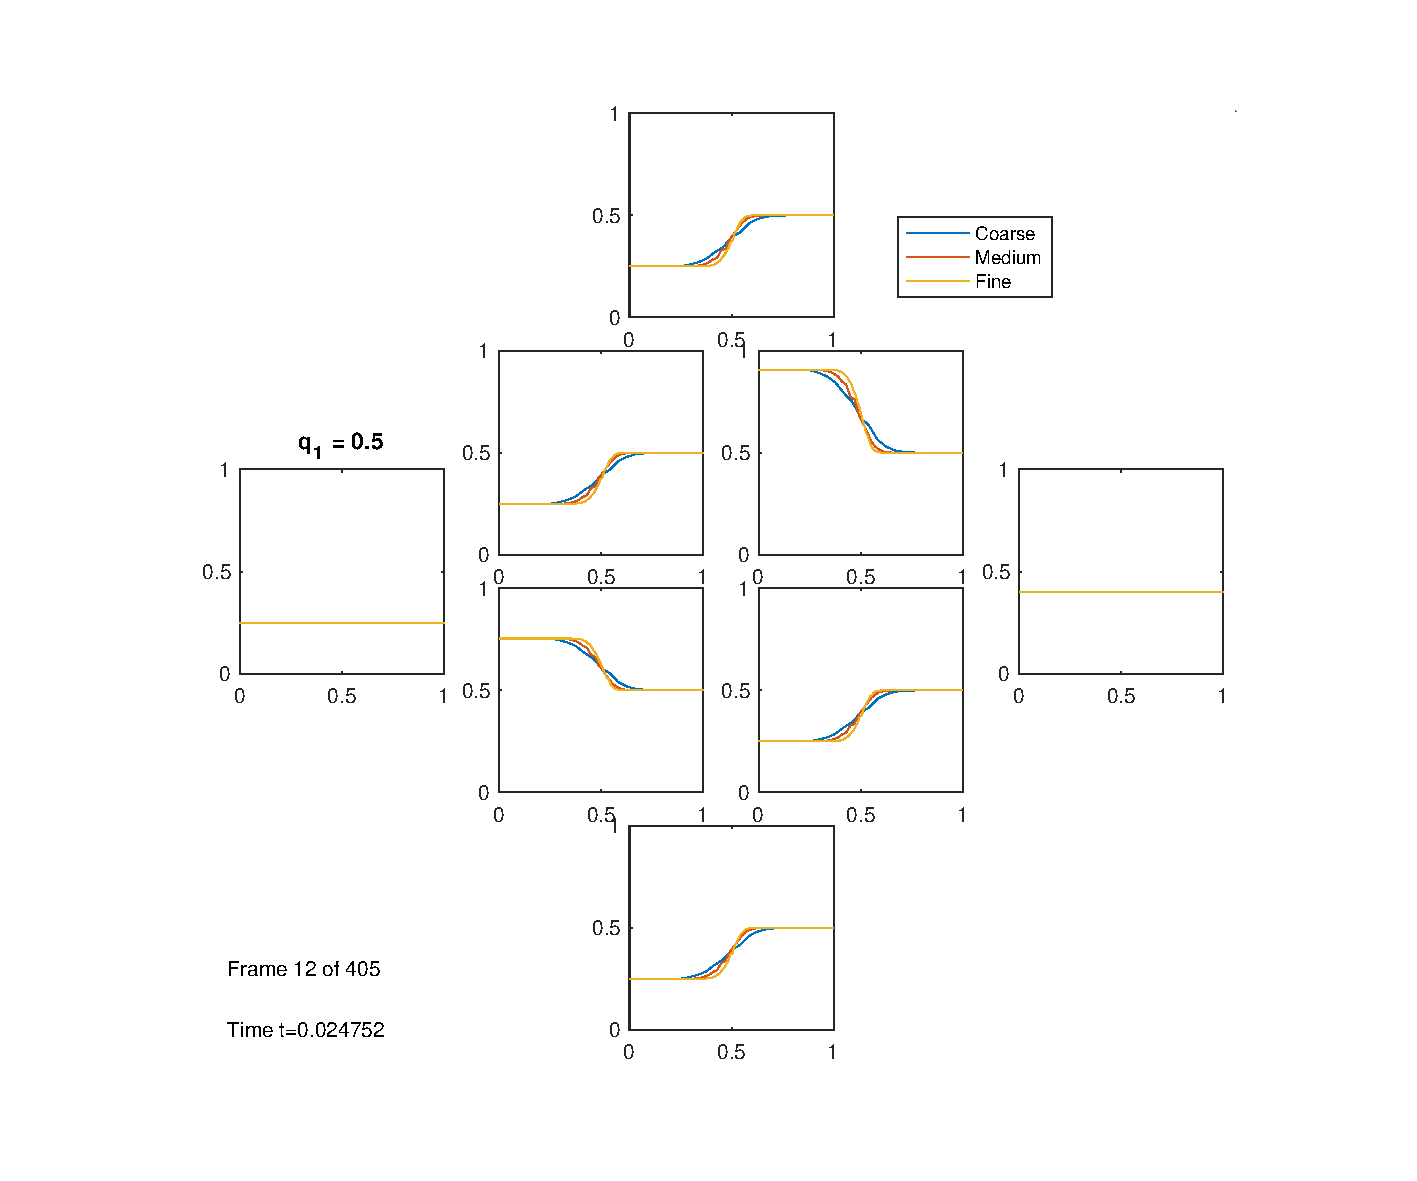
\includegraphics[trim=80 50 80 50,clip,width=0.75\textwidth]{trafficCircles3.pdf}
		\caption[Traffic Circles : Spatial refinement]{Coarse to fine respectively represents $dx=0.02,0.01,0.005$. Increasing the spatial increment causes discontinuities to be resolved more accurately, coarse grids dissipate the density shock.}
		\label{fig:randd:traffic_circles_dx}
	\end{figure}
	\begin{figure}
    		\centering
        		\includegraphics[trim=140 85 135 70,clip,width=\textwidth]{trafficcircles_Limiters.pdf}
		\caption[Traffic Circles : MUSCL limiters]{Various slope limiters applied to MUSCL reconstruction on the traffic circle case. The top and bottom rows represent the density solution on the leftmost inlet road with second and third order MUSCL reconstructions respectively. The VanAlbada2 limiter becomes numerically unbounded after 10 and 35 time steps for 2nd and 3rd order reconstructions respectively.}
		\label{fig:randd:traffic_circles:limiters}
	\end{figure}

\section{Real Road Networks}

	Following the theoretical networks used to test the models numerical and probabilistic capabilities, these sections show how the simulations work when reproducing traffic behaviour on real road network sections. The Piazza dei Re Di Roma roundabout in southeast Rome, and a common UK motorway junction taken from the M1 near Leeds.

\subsection{Re Di Roma Roundabout}

	This road section is studied in \cite{Bretti07}, and resembles a more realistic traffic circle as in Section \ref{randd:trafficcircles}. Figure \ref{fig:randd:RDR:map} shows the network surrounding the roundabout from Google Maps. As this network is real, the postprocessing involving a real road network simulation needs to be more aesthetic than density profile plots. Figure \ref{fig:randd:rediroma} shows the result from an initial simulation using the Re Di Roma roundabout. This figure shows the density not as a distribution but through colour of a physical diagram of the network, the MATLAB code used to generate these figures is given in Appendix \ref{code:ReDiRoma}. Frames from this initial simulation are used to generate the animation \emph{ReDiRoma.mp4}. The parameters used for this simulation result in the solution developing (Figure \ref{fig:randd:rediromaA}) and reaching a steady state (Figure \ref{fig:randd:rediromaB}). These results use first order cell reconstruction with the Lax-Friedrichs Riemann solver. The following results test other numerical methods on the Re Di Roma network, only showing the solution for the central roundabout in polar coordinates the density is shown by the distance from the black circle.
	\\ \\
	As this real network has road segments of irregular length, choosing an arbitrary spatial increment $dx$ can cause the postprocessing to be out of sync when comparing two solutions. Figure \ref{fig:randd:rediroma:grids} shows the roundabout density solution with different spatial resolutions, the coarse simulation is slightly out of sync due to the length of the road network not being divisible into an integer number of cells. For this reason, the coarse profile is smoothed over the density jumps resulting from traffic coming in to the roundabout from source roads. The drops in density are equivalently from sink roads leaving the roundabout. The fine simulation predicts the density jump locations more accurately than both medium and fine. The south-southwest region of the roundabout has an increase of density, shown by the fine and medium solutions, however the coarse solution smooths this small increase in density so much that it could be interpreted differently if analysed without the finer solutions to compare to.
	\\ \\
	The analysis of reconstruction methods on the Re Di Roma roundabout is shown at two stages during the simulation in Figure \ref{fig:randd:rediroma:reco}. This physical postprocessing method makes identifying shock capturing accuracy difficult, however is used to show the application to real networks. On the south of the roundabout (left figure), it is evident that the 3$^{rd}$ order WENO reconstruction captures a stronger shock than the second order and first order as expected. It is useful to know these reconstruction methods are behaving as expected even when embedded in a large program that is solving a complicated process defined on an equally complicated real road network. Later in the simulation (right figure) the solution is becoming more smooth so the effect of reconstruction is not as significant. 
	\\ \\
	We have already seen from simulations on the traffic circle, and in Figure \ref{fig:randd:traffic_circles_riemann}, that the choice of Riemann solver has little influence. Figure \ref{fig:randd:rediroma:riem} shows this is also the case for the Re Di Roma roundabout case. The solution for the HLL and Murman-Roe solvers are equivalent with the Lax-Friedrichs solution differing only very slightly. It is clear that the definition of Riemann solvers in traffic flow network modelling simulations needs to be decided more carefully. 
	
	\begin{figure}
    		\centering
        		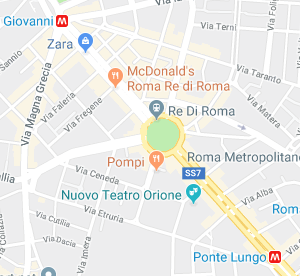
\includegraphics[trim=0 0 0 0,clip,width=0.57\textwidth]{RDR_map.png}
		\caption[Re Di Roma : Junction area map]{Central Rome roundabout network. \emph{Google Maps, 2019.}}
		\label{fig:randd:RDR:map}
	\end{figure}

	\begin{figure}
  		\centering
  		\subfloat[Developing flow]{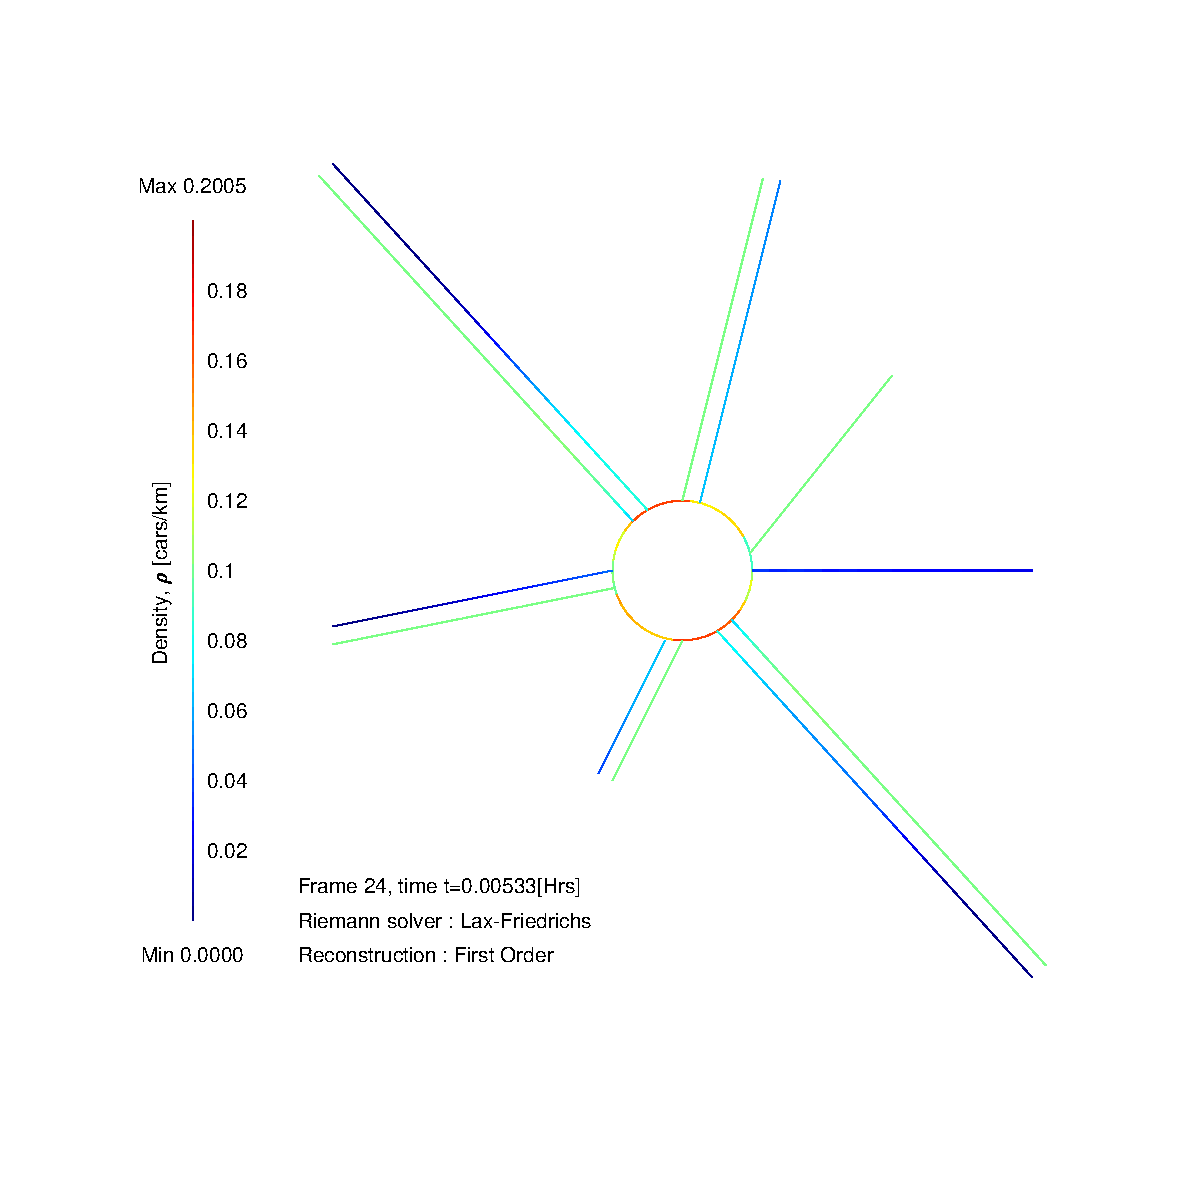
\includegraphics[trim=135 95 64 75,clip,width=0.45\textwidth]{ReDiRoma2.pdf}\label{fig:randd:rediromaA}}
  		\hfill
  		\subfloat[Steady traffic distribution]{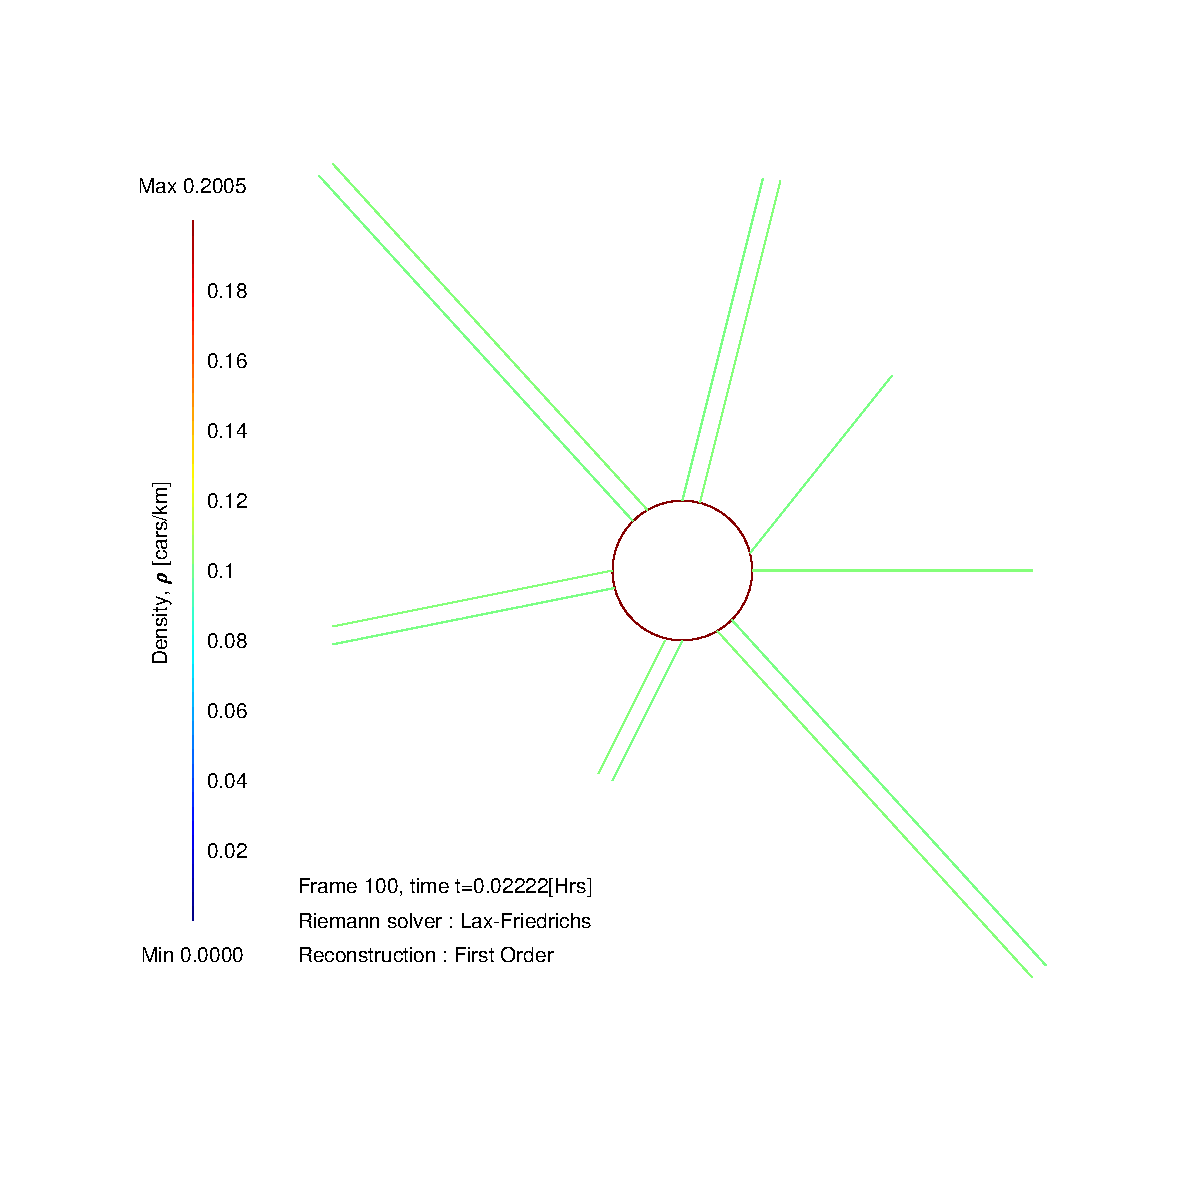
\includegraphics[trim=65 95 64 75,clip,width=0.53\textwidth]{ReDiRoma3.pdf}\label{fig:randd:rediromaB}}
  		\caption[Re Di Roma : Density line contour]{From the initially empty distribution, traffic flows towards the roundabout (a) and reaches a steady density profile (b).  \label{fig:randd:rediroma}}
	\end{figure}
	
	\begin{figure}
    		\centering
        		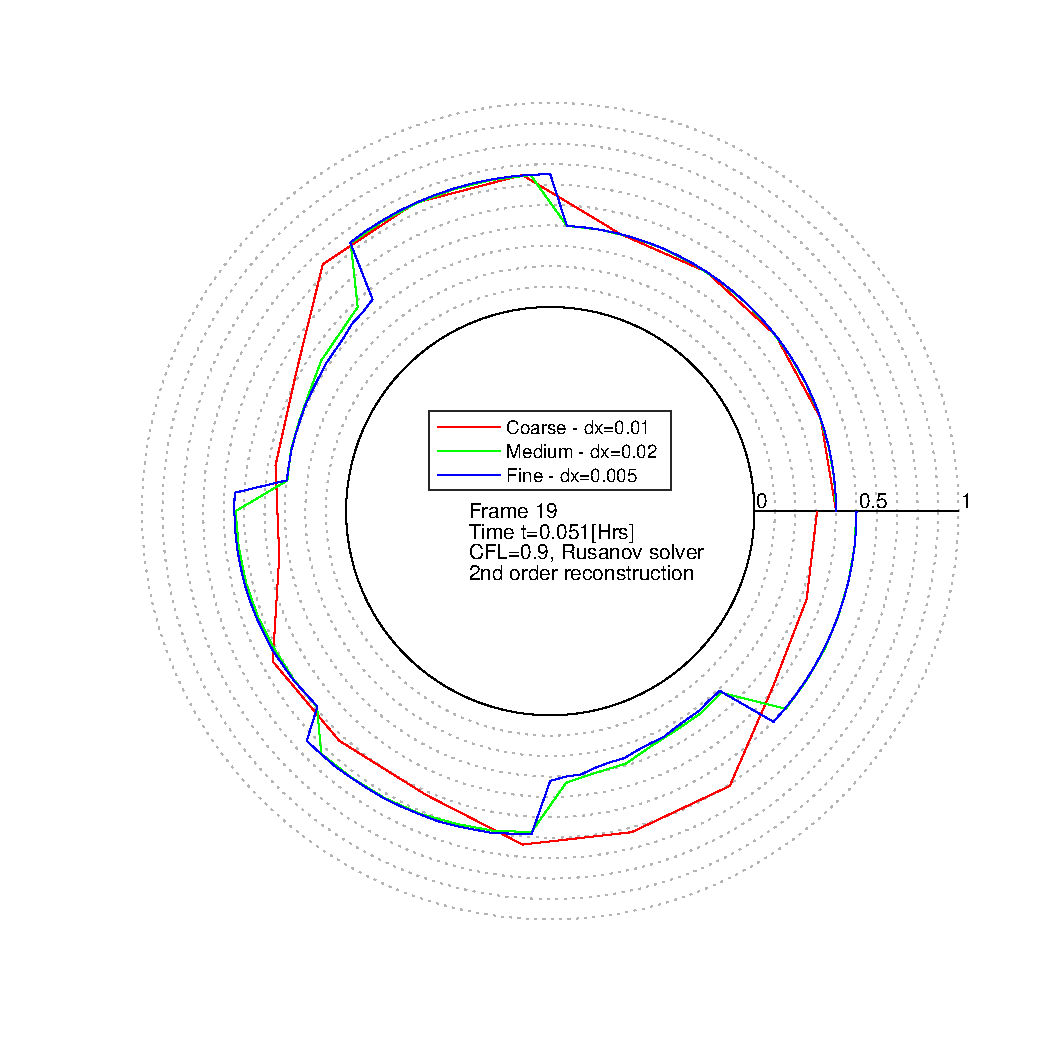
\includegraphics[trim=60 60 40 40,clip,width=0.8\textwidth]{ReDiRoma_grid.pdf}
		\caption[Re Di Roma : Grid resolution]{As expected the finer grid resolves jumps in density from oncoming roads well, the coarse grid is such that it smooths or even misses density jumps completely due to the resolution of the simulation.}
		\label{fig:randd:rediroma:grids}
	\end{figure}
	
	\begin{figure}
    		\centering
        		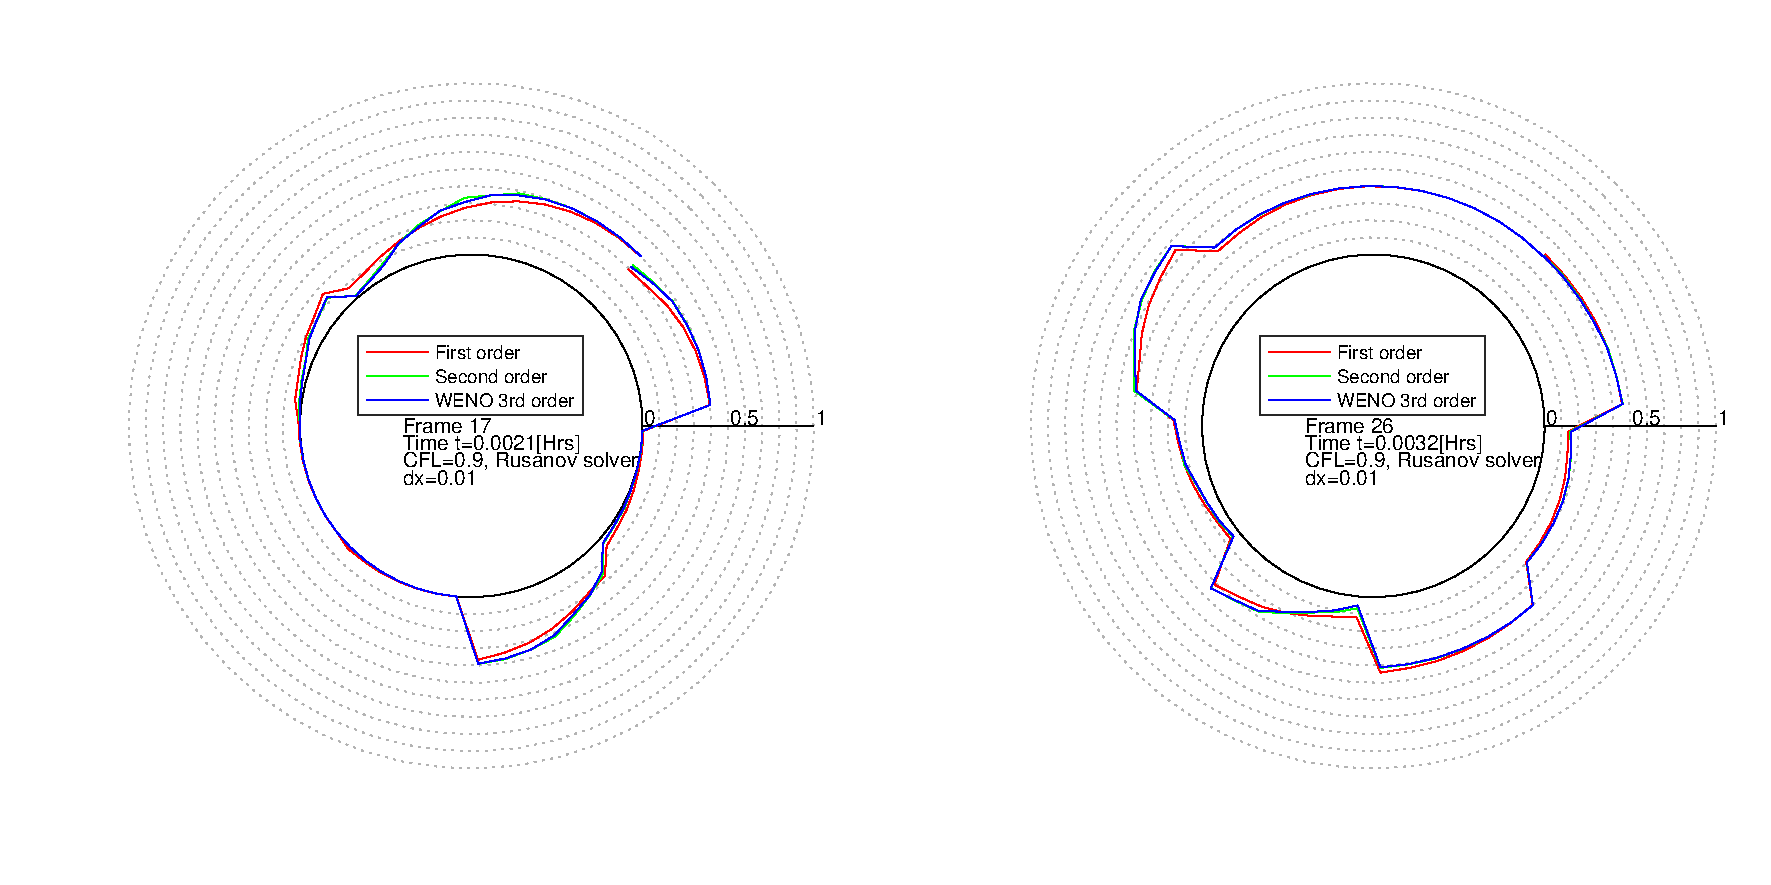
\includegraphics[trim=60 55 20 40,clip,width=\textwidth]{ReDiRoma_reco.pdf}
		\caption[Re Di Roma : Reconstruction]{Two time steps at frame 17 (left) and 26 (right) of traffic density feeding through the Re Di Roma central roundabout. Lower order reconstruction methods smooth out discontinuities at junctions whereas the higher order methods resolve jumps more accurately.}
		\label{fig:randd:rediroma:reco}
	\end{figure}
	
	\begin{figure}
    		\centering
        		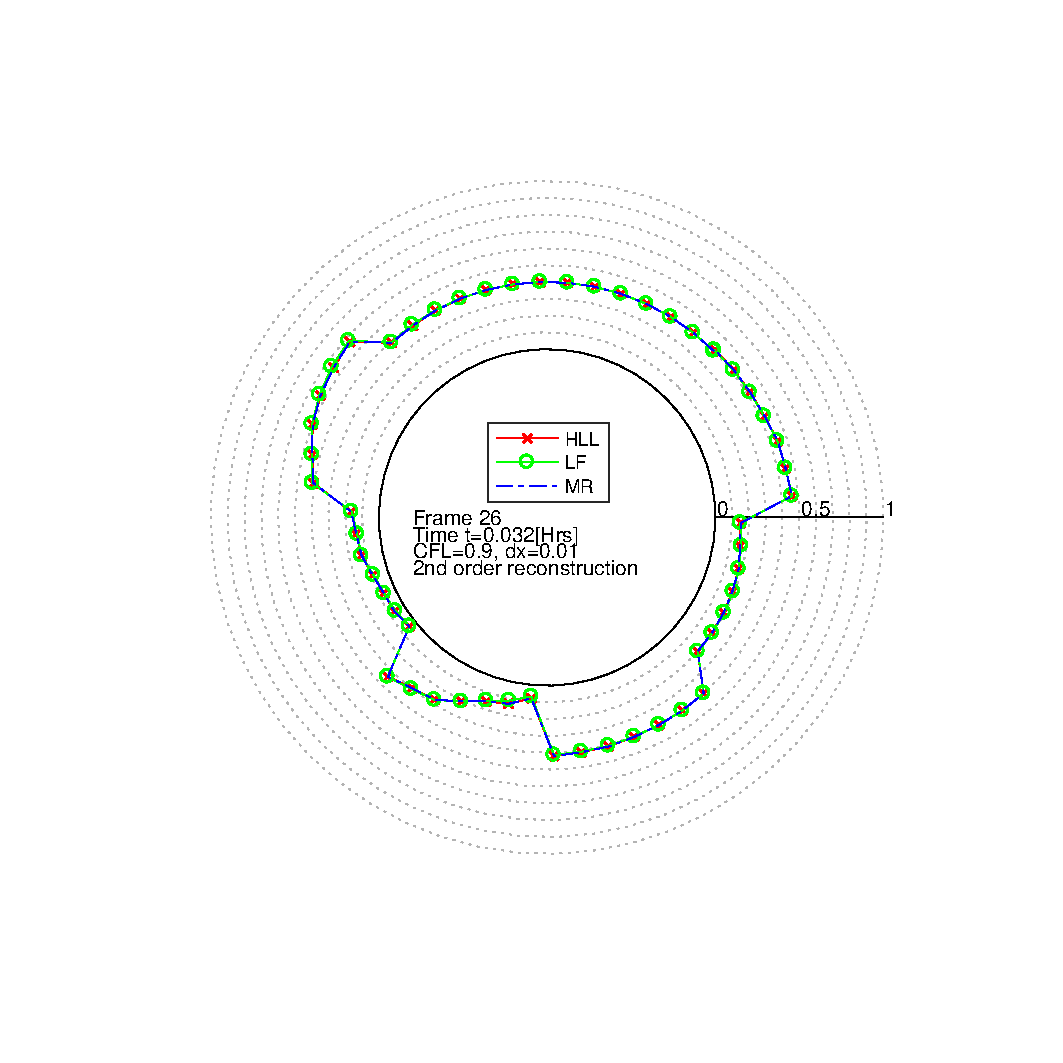
\includegraphics[trim=100 100 80 80,clip,width=0.8\textwidth]{ReDiRoma_riem.pdf}
		\caption[Re Di Roma : Riemann solvers]{The choice of Riemann solver results in a negligible difference in solution. The HLL and Murman-Roe (MR) solver solutions are identical and Lax-Friedrichs (LF) differs only very slightly.}
		\label{fig:randd:rediroma:riem}
	\end{figure}
	
\subsection{Wakefield M1 Junction 40}
\label{sec:randd:M1J40}

	The common simple UK motorway junction meets a crossing A-road at right angles and the model junction can be described by junction 40 of the M1 in Wakefield. Figure \ref{fig:randd:M1J40:map} shows the small interchange network surrounding the meeting of a fast high-density motorway taking traffic to and from London, the Midlands and Leeds. This network is a good example of when a time-dependent TDM may be useful to model over a long time period such as 24 hours. During the morning hours lots of traffic may be coming from all directions towards Leeds, and the opposite in the evening rush hour at high densities. This map has been traced in MATLAB and used for postprocessing (Appendix \ref{code:m1j40})for the initial simulation results, which can be found in Figure \ref{fig:randd:M1J40}. Not only is the line drawing of the motorway junction coloured by high and low local densities, but the higher density regions are matched with a thicker line. This simulation uses first order reconstruction with Lax-Friedrichs numerical flux calculations. Frames from this initial simulation are used to generate the animation \emph{M1J40.mp4}. This figure allows the clear identification of a high local density on the southbound lane of the motorway after traffic rejoins from the A roads and the roundabout slip road. The following results use more classical postprocessing and analyse the influence of the CFL number, and reconstruction around the motorway and slip lanes.
	\\ \\
	The southbound motorway lane and its slip lane off to the junction roundabout are shown in Figure \ref{fig:randd:M1J40:cfl}, with 4 profiles for different values of the CFL constraint which defines the time resolution from the spatial resolution. The main motorway section shows a spike in density just before the slip lane begins, after which the slip lane density begins to increase. This is not as expected and may be due to a fault in the junction solver. In terms of the CFL influence on solution accuracy, lower CFL give rise to a more accurate capturing of the density jump along the motorway section that has not departed off the slip lane. 
	\\ \\
	The spike observed in Figure \ref{fig:randd:M1J40:cfl} cannot be due to the reconstruction interference at junctions as Figure \ref{fig:randd:M1J40:reco} shows the same spike for many reconstruction methods. This figure shows the whole southbound M1 lane with off and on slip roads. The two drops in density at 100 and 170 are due to the inlet flow of the southbound motorway not leaving the off-slip road, and flow from the A road joining the motorway from the on-slip road respectively. The 5$^{th}$ order WENO scheme gives a small increase before the main drop in density, this is not seen in the 3$^{rd}$ or bounded 7$^{th}$ schemes. The 3$^{rd}$ order MUSCL scheme appears to be less accurate than the 2$^{nd}$ order, which from Figure \ref{fig:randd:traffic_circles:limiters} we can conclude that with a more sensible choice of slope limiter, the 3$^{rd}$ order MUSCL scheme will behave better. A different slope limiter may also reduce some of the oscillations in the density drop with this MUSCL reconstruction. We can also see that the smaller drop in density from 0.3 to 0 gives rise to a less smooth 7$^{th}$ order WENO reconstruction, when compared to the larger earlier jump. 
	
	\begin{figure}
    		\centering
        		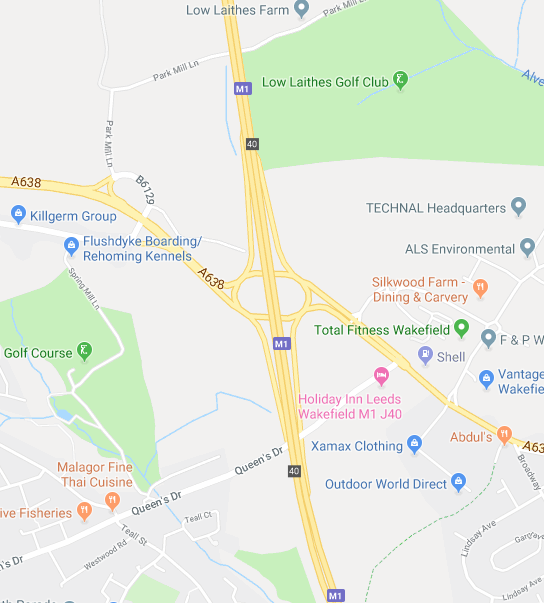
\includegraphics[trim=0 0 0 0,clip,width=0.58\textwidth]{M1J40.png}
		\caption[Wakefield M1J40 : Junction area map]{Simple and common UK motorway and A-road junction. \emph{Google Maps, 2019.}}
		\label{fig:randd:M1J40:map}
	\end{figure}

	\begin{figure}
    		\centering
        		\subfloat[Developing]{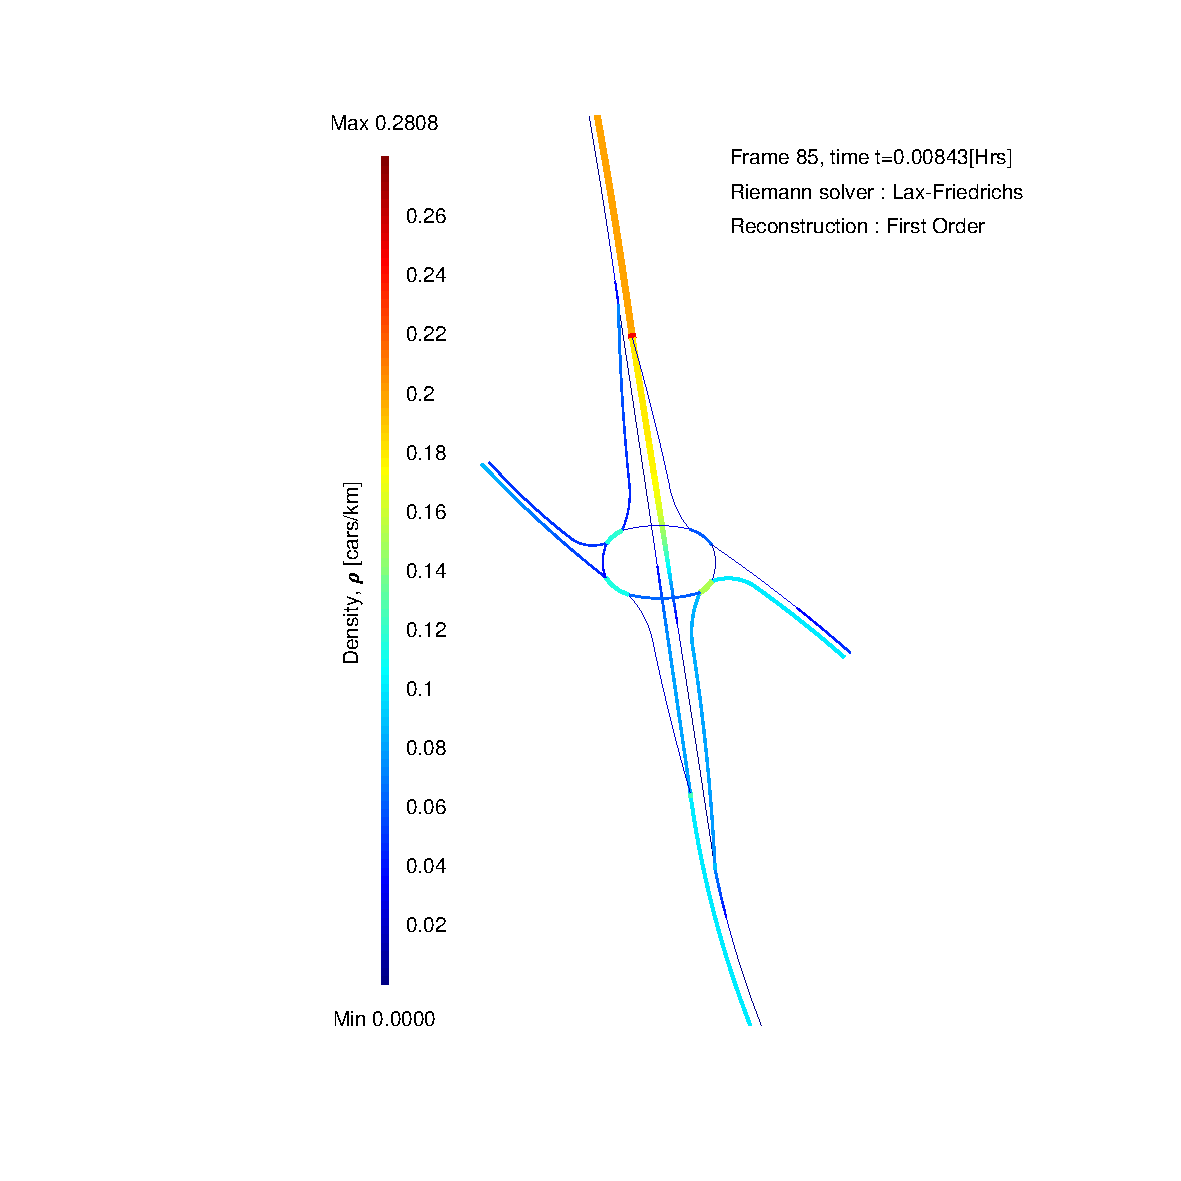
\includegraphics[trim=230 70 70 50,clip,width=0.426\textwidth]{M1J40_1.pdf}\label{fig:randd:M1J40:dev}}
        		\hfill
        		\subfloat[Steady]{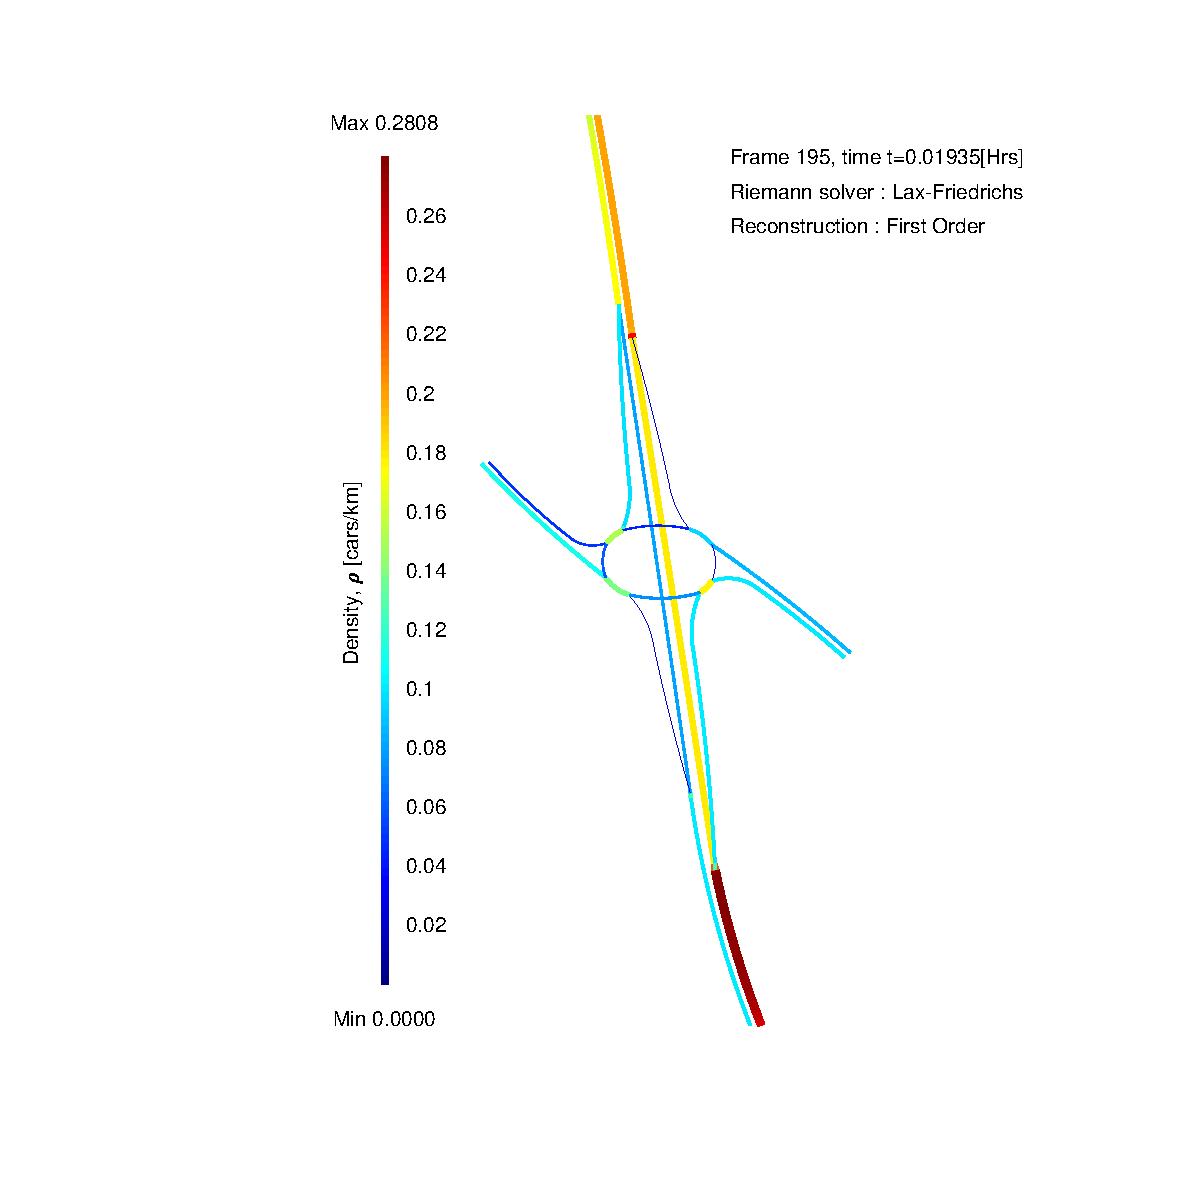
\includegraphics[trim=150 70 70 50,clip,width=0.553\textwidth]{M1J40_2.pdf}\label{fig:randd:M1J40:steady}}
		\caption[Wakefield M1J40 : Density line contour]{Heavy flow southbound from Leeds towards Wakefield and further south. Highlighting the higher density areas of the motorway junction roundabout.\label{fig:randd:M1J40}}
	\end{figure}
	
	\begin{figure}
    		\centering
        		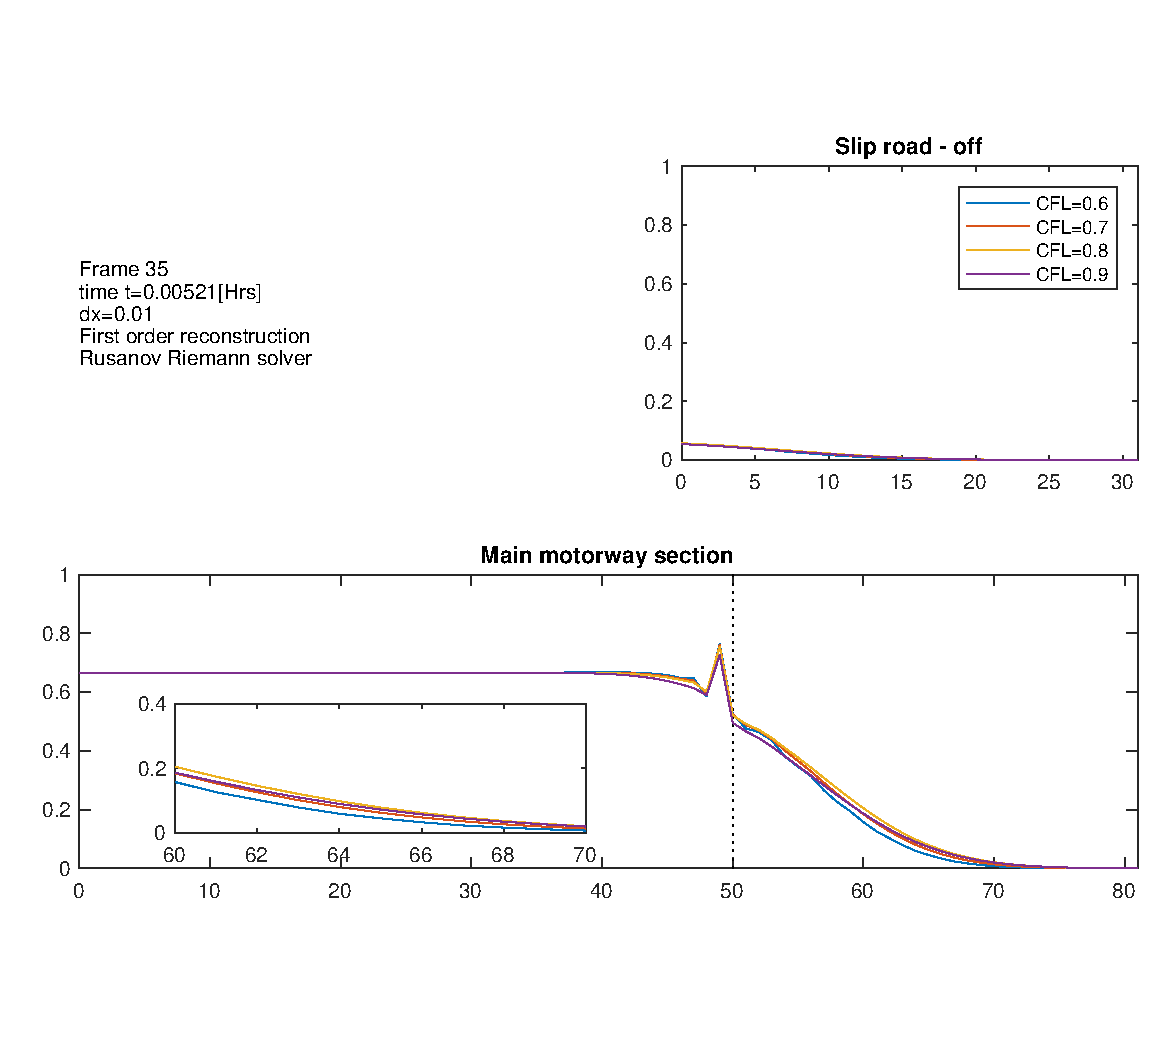
\includegraphics[trim=20 75 10 55,clip,width=0.93\textwidth]{M1J40_cfl.pdf}
		\caption[Wakefield M1J40 : Density profile for varying $CFL$]{The influence of $CFL$ number is little, there are oscillations present at the slip road entrance for all $CFL$. The value $CFL=0.6$ appears to capture the traffic density jump with highest gradient. These simulations are analysed by simulation time in Figure \ref{fig:randd:Time:M1J40_CFL}}
		\label{fig:randd:M1J40:cfl}
	\end{figure}
	
	\begin{figure}
    		\centering
        		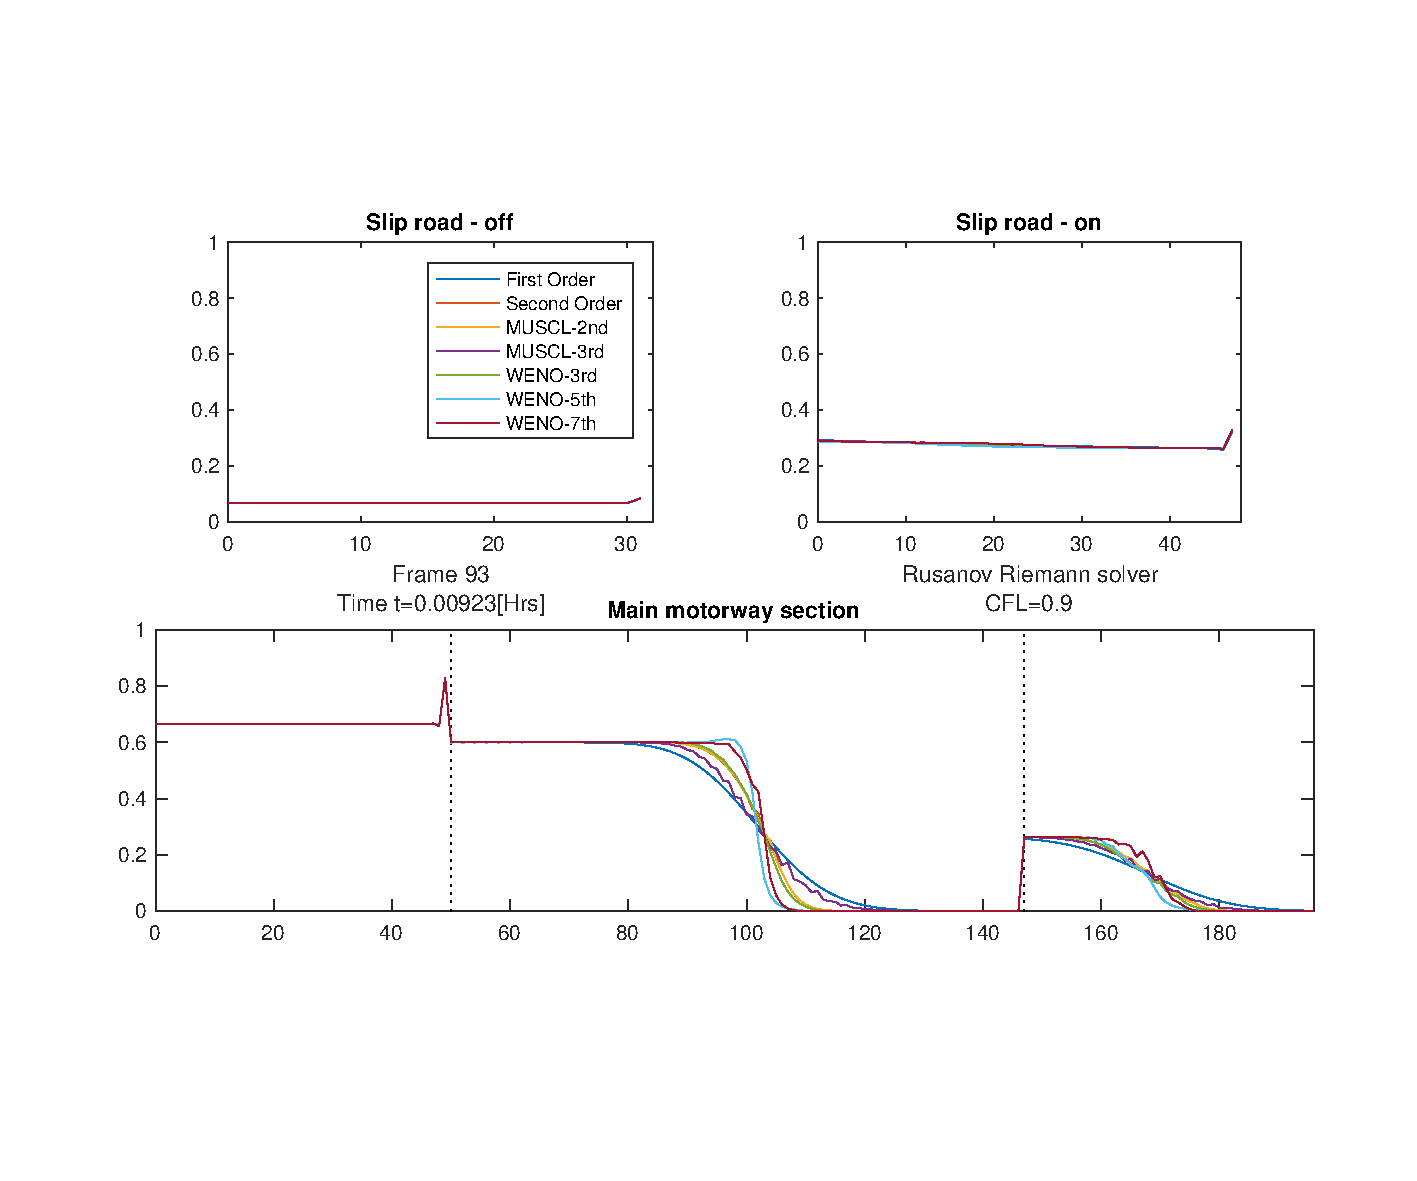
\includegraphics[trim=57 110 40 100,clip,width=\textwidth]{M1J40_reco.pdf}
		\caption[Wakefield M1J40 : Density profile for varying reconstruction]{$dx=0.01$. This figure shows the southbound motorway lane with two slip roads towards and away from the roundabout. Reconstruction appears to have a significant influence on the accurate capturing of a jump in traffic density. The general pattern is a more accurate shock resolution for higher order schemes, however this comes at the cost of computational time and oscillations.}
		\label{fig:randd:M1J40:reco}
	\end{figure}

\section{Time Analysis}
\label{sec:randd:timeanalysis}

	A high resolution numerical scheme can be highly time-costly,  and when such a numerical scheme is coupled with a large road network as the domain this cost is multiplied. It is therefore important to analyse which aspects or parameters of a simulation cause changes in the computational time. The following results are taken from the simulation information output, see Appendix \ref{txt:info:output} , with a total time and a breakdown of the time spent on reconstruction and solving local Riemann problems for example. 
	\\ \\
	The analysis of the 7$^{th}$ order WENO scheme in Section \ref{randd:singleroad} and Figure \ref{fig:randd:single:7thOrder} is followed by Figure \ref{fig:randd:Time:SingleRoadW7}. This shows how the higher order WENO schemes vary in terms of total simulation time (orange) and the time-breakdown on simulations of the single road segment. With high resolution reconstruction methods, the reconstruction time will dominate the simulation and the total time is reflected by this. The unbounded 7$^{th}$ order scheme saves time over the bounded solution by not computing the bounds themselves, but as seen in Figure \ref{fig:randd:single:7thOrder} this saving is not worth the cost of a meaningless solution. The monotonic bounding from Balsara and Shu \cite{BalsaraShu00} is essential for the 7$^{th}$ order WENO reconstruction.
	\\ \\
	The alternate MUSCL reconstruction method also has an important parameter which contributes to both computational speed and solution accuracy. The MUSCL slope limiter as in Section \ref{sec:HRS} and Appendix \ref{ap:MUSCLslopelim} is a simple tool such that can easily be written into any program to be varied and tested for solution (Figure \ref{fig:randd:traffic_circles:limiters}) and in Figure \ref{fig:randd:Time:traffic_circles:limiters}, for computational time. We identified the Monotonised Central \cite{VanLeer77} and UMIST \cite{Lien94} limiters as the most admissible in terms of density jump capturing accuracy on the traffic circles network, and in this figure it is clear that these two schemes increase the computational cost. The VanLeer \cite{VanLeer74} limiter can be seen here to be one of the quickest, and in Figure \ref{fig:randd:traffic_circles:limiters} is identified as a high accuracy limiter with a smooth and high gradient density drop. This figure also shows the difference in cost when limiters are applied to the 2$^{nd}$ or 3$^{rd}$ order MUSCL schemes, of which all limiters show a similar small increase in time and all 3$^{rd}$ order total times are greater than 3$^{rd}$ order totals as expected. The VanLeer \cite{VanLeer74} limiter however has a slightly smaller 3$^{rd}$ order speed-up.  
	\\ \\
	The final time analysis from the traffic circles network is that of spatial resolution, the time taken for solutions shown in Figure \ref{fig:randd:traffic_circles_dx} and more values of $dx$ are simulated and the time breakdown is shown here in Figure \ref{fig:randd:Time:traffic_circles:grid}. It is expected that with a finer spatial resolution, the road network is described by a greater number of computational cells which will result in more calculations and a greater simulation time. With a second order reconstruction it is interesting to see that it is the local Riemann solutions that begin to dominate the total simulation time for the smallest $dx$ simulated here. At the largest $dx=0.175,0.2$ the reconstruction and flux times appear very similar. As with most numerical simulations there is a compromise between solution accuracy and computational time, here a value of $dx=0.05$ gives a valuable solution and saves 75\% of the $dx=0.025$ simulation time. 
	
	\newpage
	
	\begin{figure}[H]
    		\centering
        		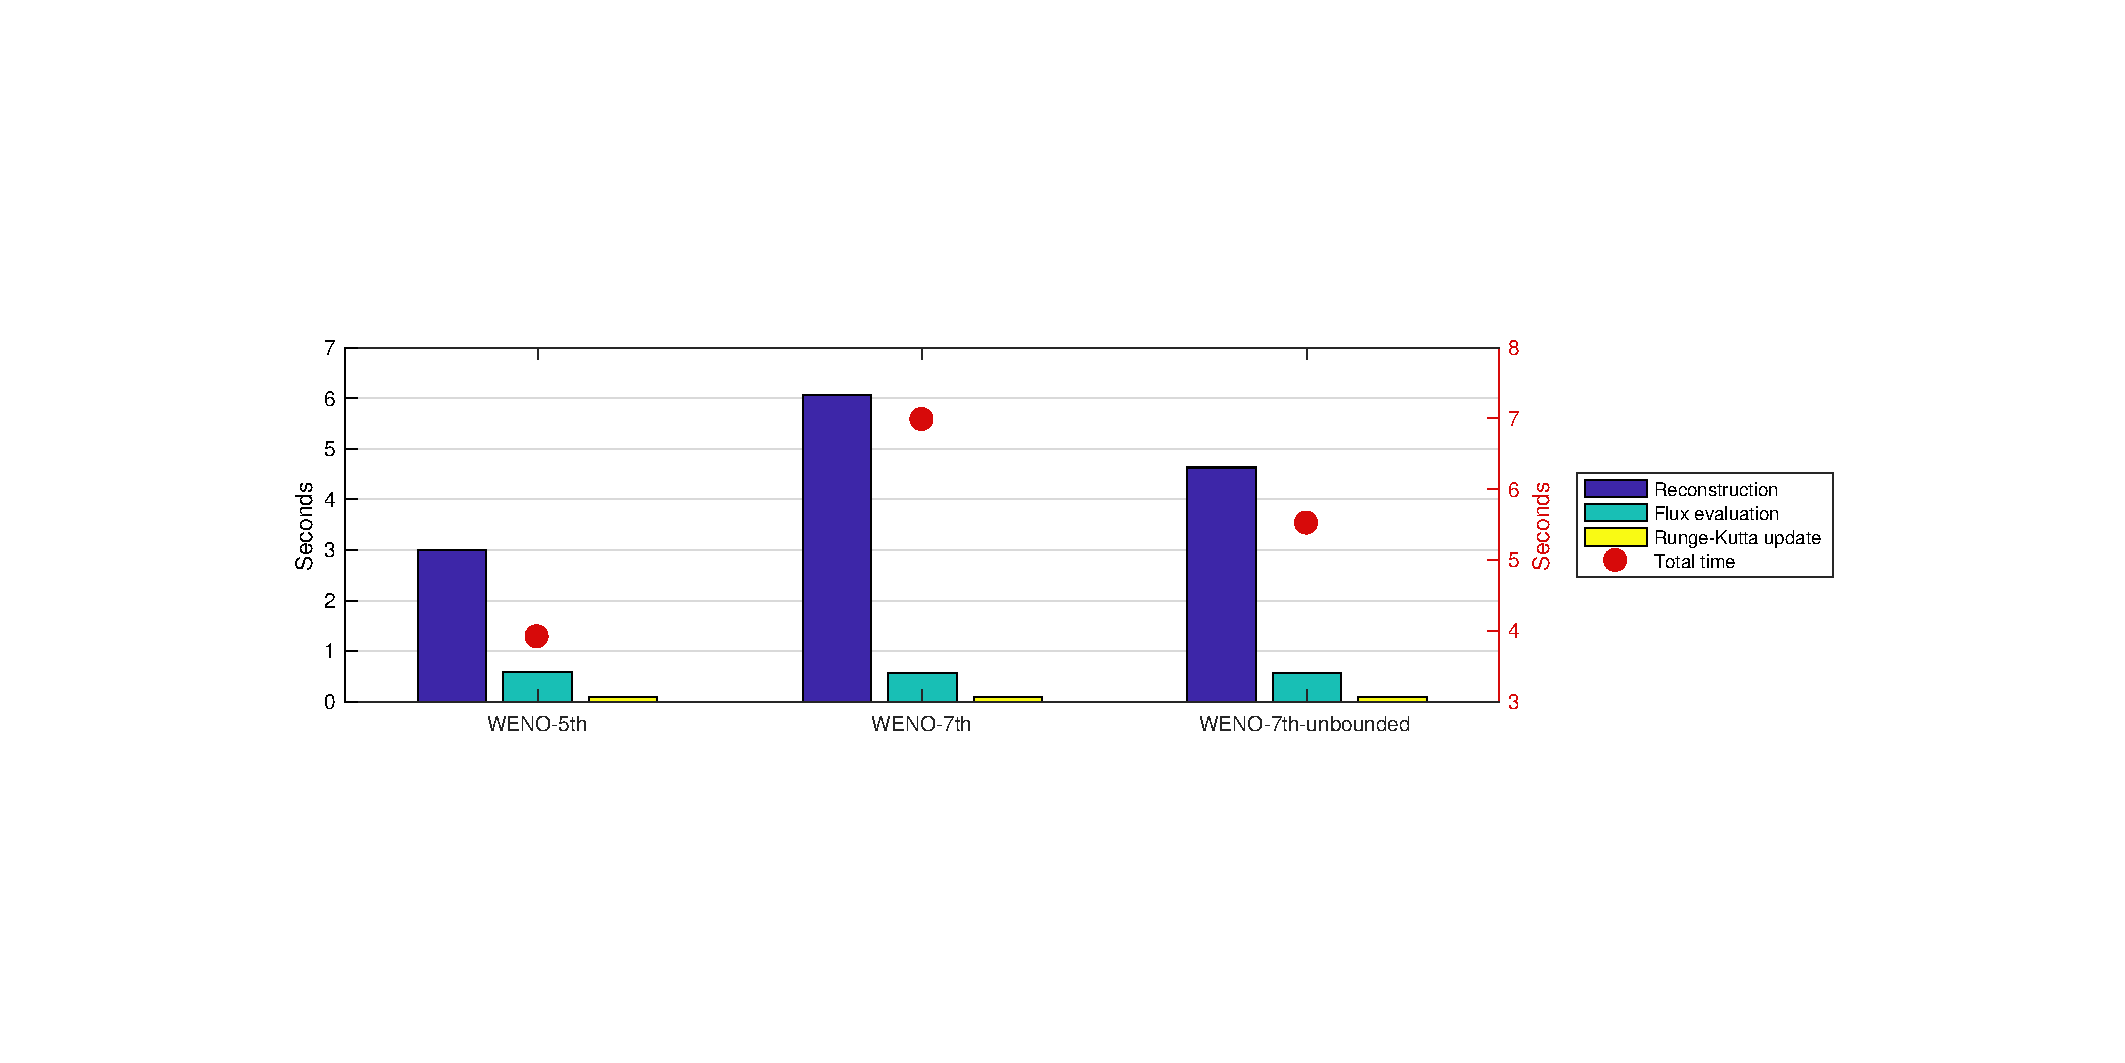
\includegraphics[trim=140 160 138 160,clip,width=\textwidth]{Time_SingleRoad_W7.pdf}
		\caption[Time Analysis : ]{As expected the $7^{th}$ order scheme has an increased computational cost over the $5^{th}$ order due to calculations over an extra stencil. The unbounded scheme is quicker as no monotonic bounds are calculated but at the cost of an inadmissible solution this cost saving is not valuable.}
		\label{fig:randd:Time:SingleRoadW7}
	\end{figure}
	
	\begin{figure}[H]
    		\centering
        		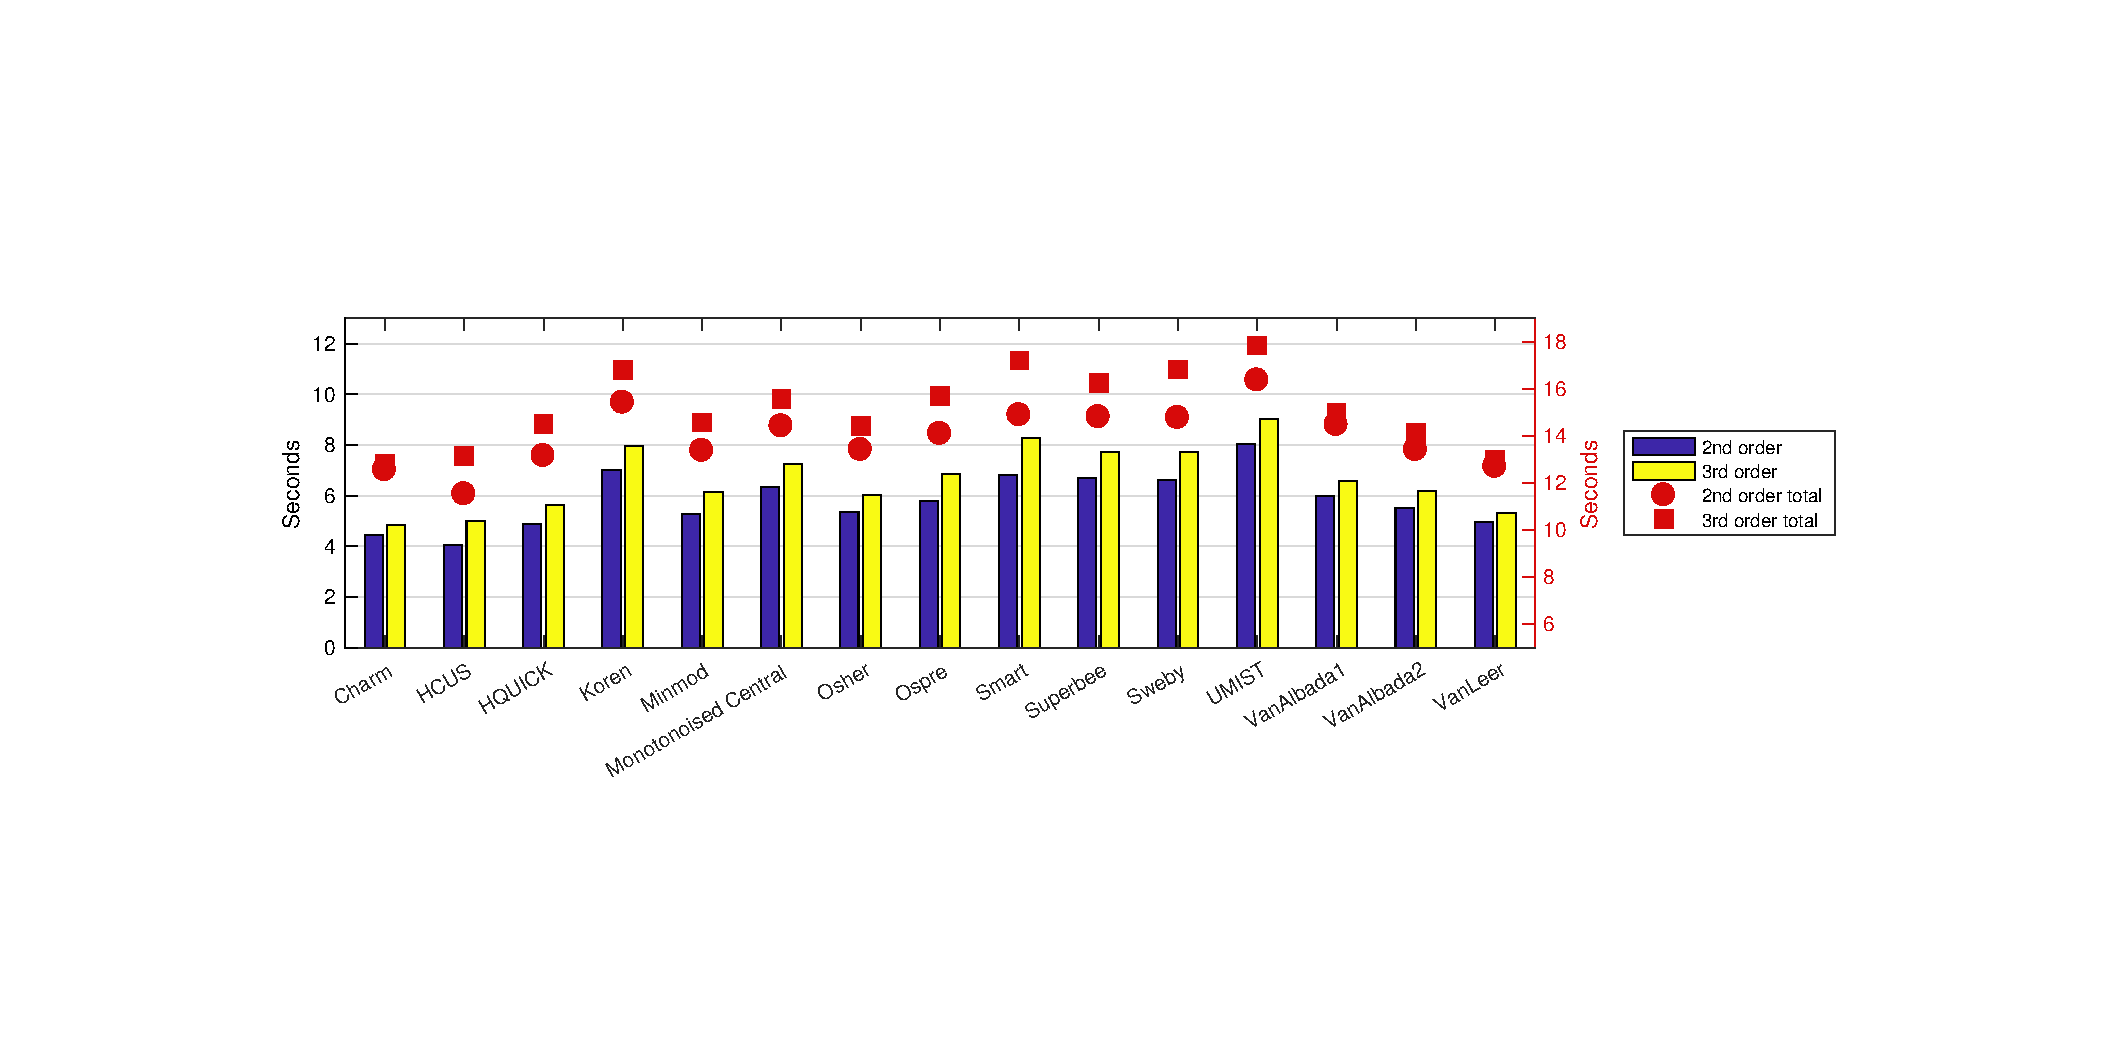
\includegraphics[trim=135 135 135 150,clip,width=\textwidth]{Time_TC_limiters.pdf}
		\caption[Time Analysis : Traffic circle slope limiters]{For all MUSCL slope limiters, the reconstruction time is shown by the bar chart and total simulation with the orange shaped marker. No limiter has a significantly higher time cost with the 3$^{rd}$ order reconstruction.}
		\label{fig:randd:Time:traffic_circles:limiters}
	\end{figure}
	
	\begin{figure}[H]
    		\centering
        		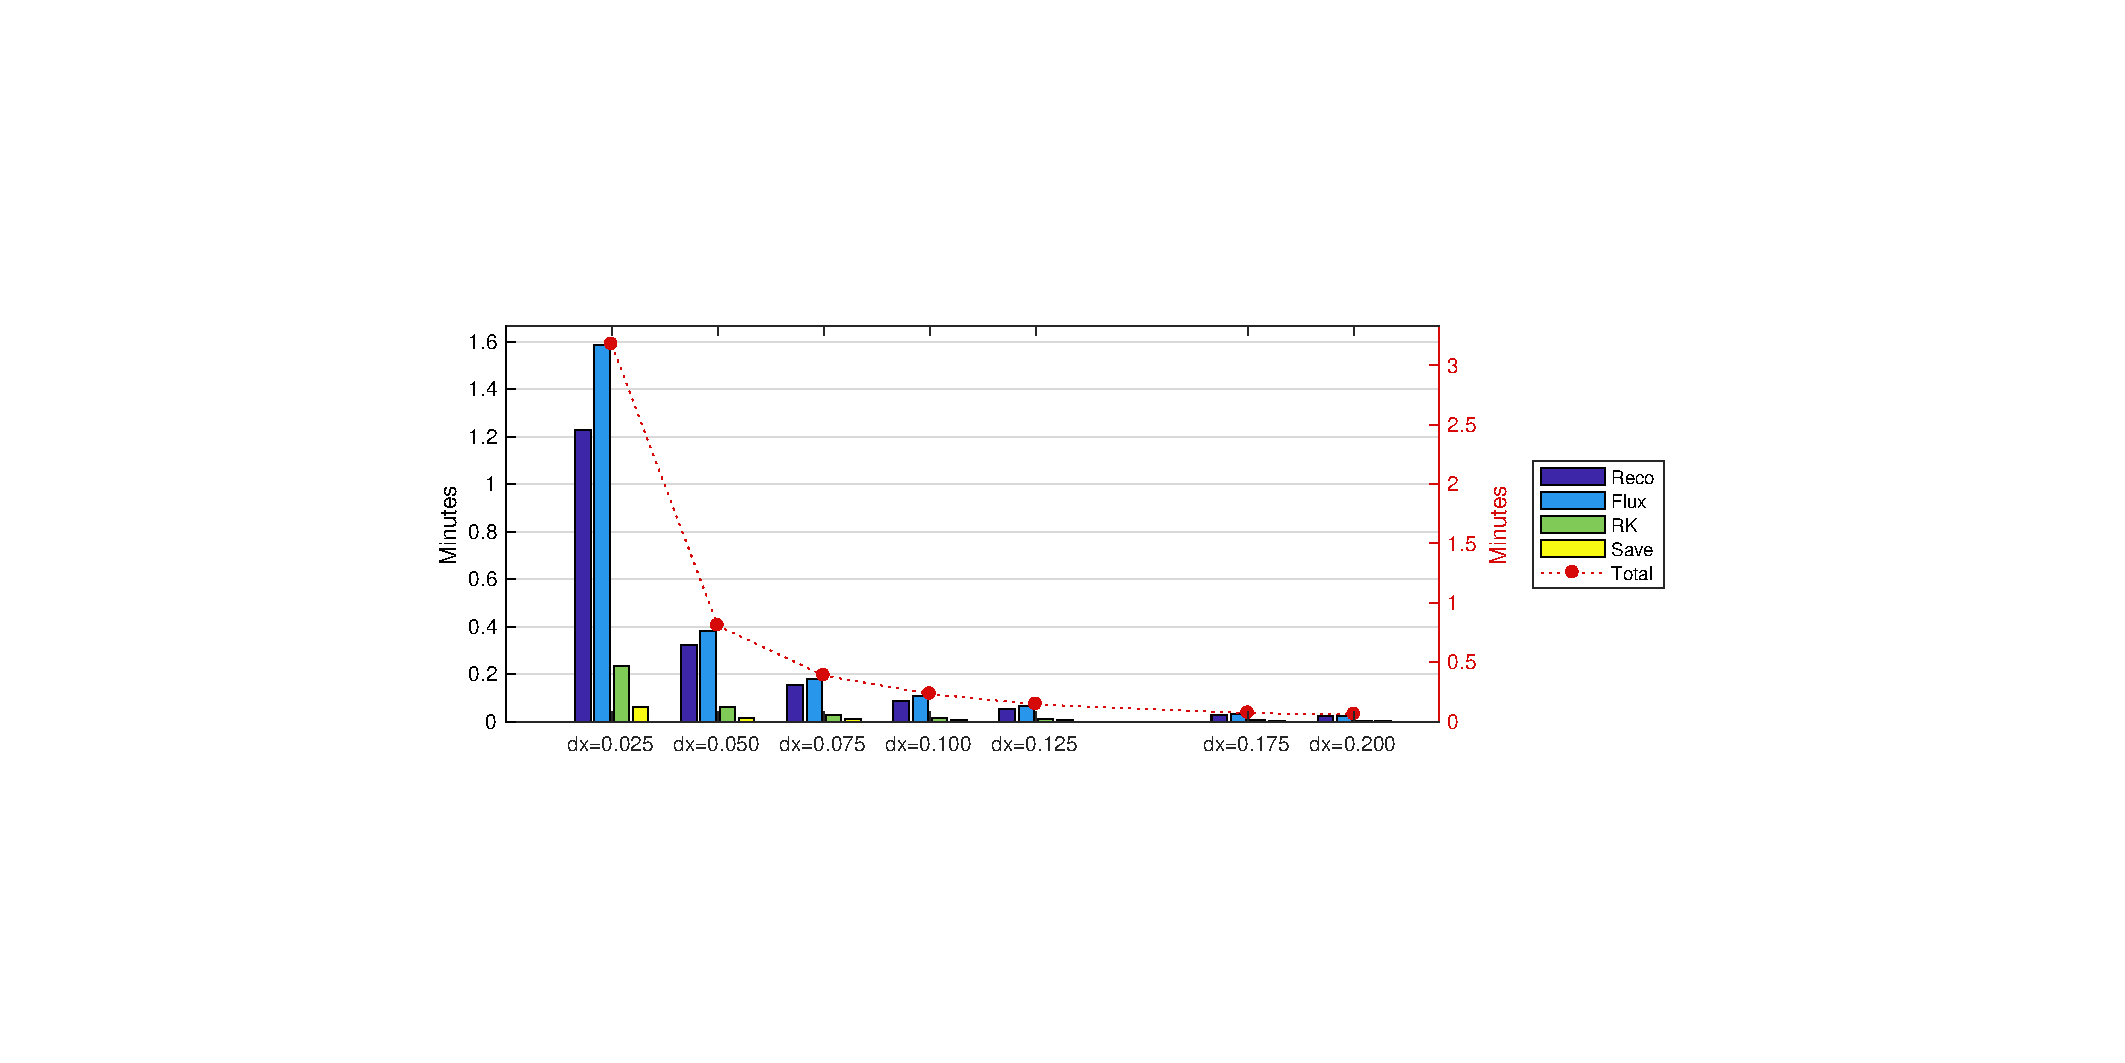
\includegraphics[trim=210 150 220 150,clip,width=\textwidth]{Time_TC_grid.pdf}
		\caption[Time Analysis : Spatial resolution]{A similar time-breakdown shows results including those from Figure \ref{fig:randd:traffic_circles_dx}, and more simulations with varying spatial resolution $dx$.}
		\label{fig:randd:Time:traffic_circles:grid}
	\end{figure}
	
	\pagebreak
	
	\noindent The next figures use time information from solutions of the Wakefield M1 junction simulations. Figure \ref{fig:randd:Time:M1J40_CFL} tests the breakdown of varying the $CFL$ constraint. With a constant $dx$, $CFL\propto dt$, so one would expect lower $CFL$ to give rise to longer computational time. This is the opposite of what is shown in Figure \ref{fig:randd:Time:M1J40_CFL}, computational time increases to a maximum at $CFL=0.8$. At this simulation setup of first order reconstruction with Rusanov flux calculations (see Figure \ref{fig:randd:M1J40:cfl}) the flux evaluations are dominating the total time, but with little difference between density profiles over each $CFL$ it may be wise to use $CFL=0.6$ to save time while also capturing the strongest density gradient along the jump.
	\\ \\
	From the analysis so far, it is not conclusive that the reconstruction influences the simulation time the most. However Figure \ref{fig:randd:Time:M1J40_reco} shows the simulation times for all available reconstruction methods in the solver parameters. With similar times for the 2$^{nd}$ order TVD and MUSCL schemes, generally the higher order reconstruction scheme will take longer to complete the reconstruction process so much that the total simulation time appears similar to the individual reconstruction time bars. After the 1$^{st}$ order scheme, all other methods total times are dominated by their reconstruction. This is as expect as higher order schemes apply extra calculations at each cell, which is multiplied over the total number of cells and time steps. The lower plot shows the relationship of the other simulation processes, these appear independent of the choice of reconstruction.
	\\ \\
	The Re Di Roma roundabout network was simulated for varying Riemann solvers, the solutions shown in Figure \ref{fig:randd:rediroma:riem}, are timed and shown here in Figure \ref{fig:randd:Time:ReDiRoma:riem}. With second order reconstruction, the Riemann solvers crucially can be more or less costly than the reconstruction procedure. In the cases of the Lax-Friedrichs and Murman-Roe solvers the flux evaluation is less costly than reconstruction whereas the HLL solver is slightly more costly than its reconstruction. The total time reflects a combination of these two important simulation procedures. Even though the Murman-Roe solver is quicker than HLL, the total times are similar due to the slower Murman-Roe reconstruction. It is hence clear that at the 2$^{nd}$ order level, the flux evaluations and reconstruction times are not independent and do influence each other. 
	\\ \\
	As with all of the time analysis thus far, it is clear that certain parameters of simulation influence the behaviour and the breakdown of total time into the key simulation sections. Figure \ref{fig:randd:Time:mixed} shows pie charts of the reconstruction, junction solver, flux evaluations, Runge-Kutta update and the saving of simulated data. The only other elements of simulation are road network definition, checking for errors and initialising the density profile, these are omitted from the pie charts as they are of the scale of $10^{-3}$ smaller than the smallest main element, the junction solver. The Wakefield motorway junction network solution with second order reconstruction (top-left) shows how dominating the reconstruction process can be, compared to a first order reconstruction process (top-right). The lower pie shows the increased flux evaluation time with the smallest grid on the traffic circles network tests. 

	\begin{figure}
    		\centering
        		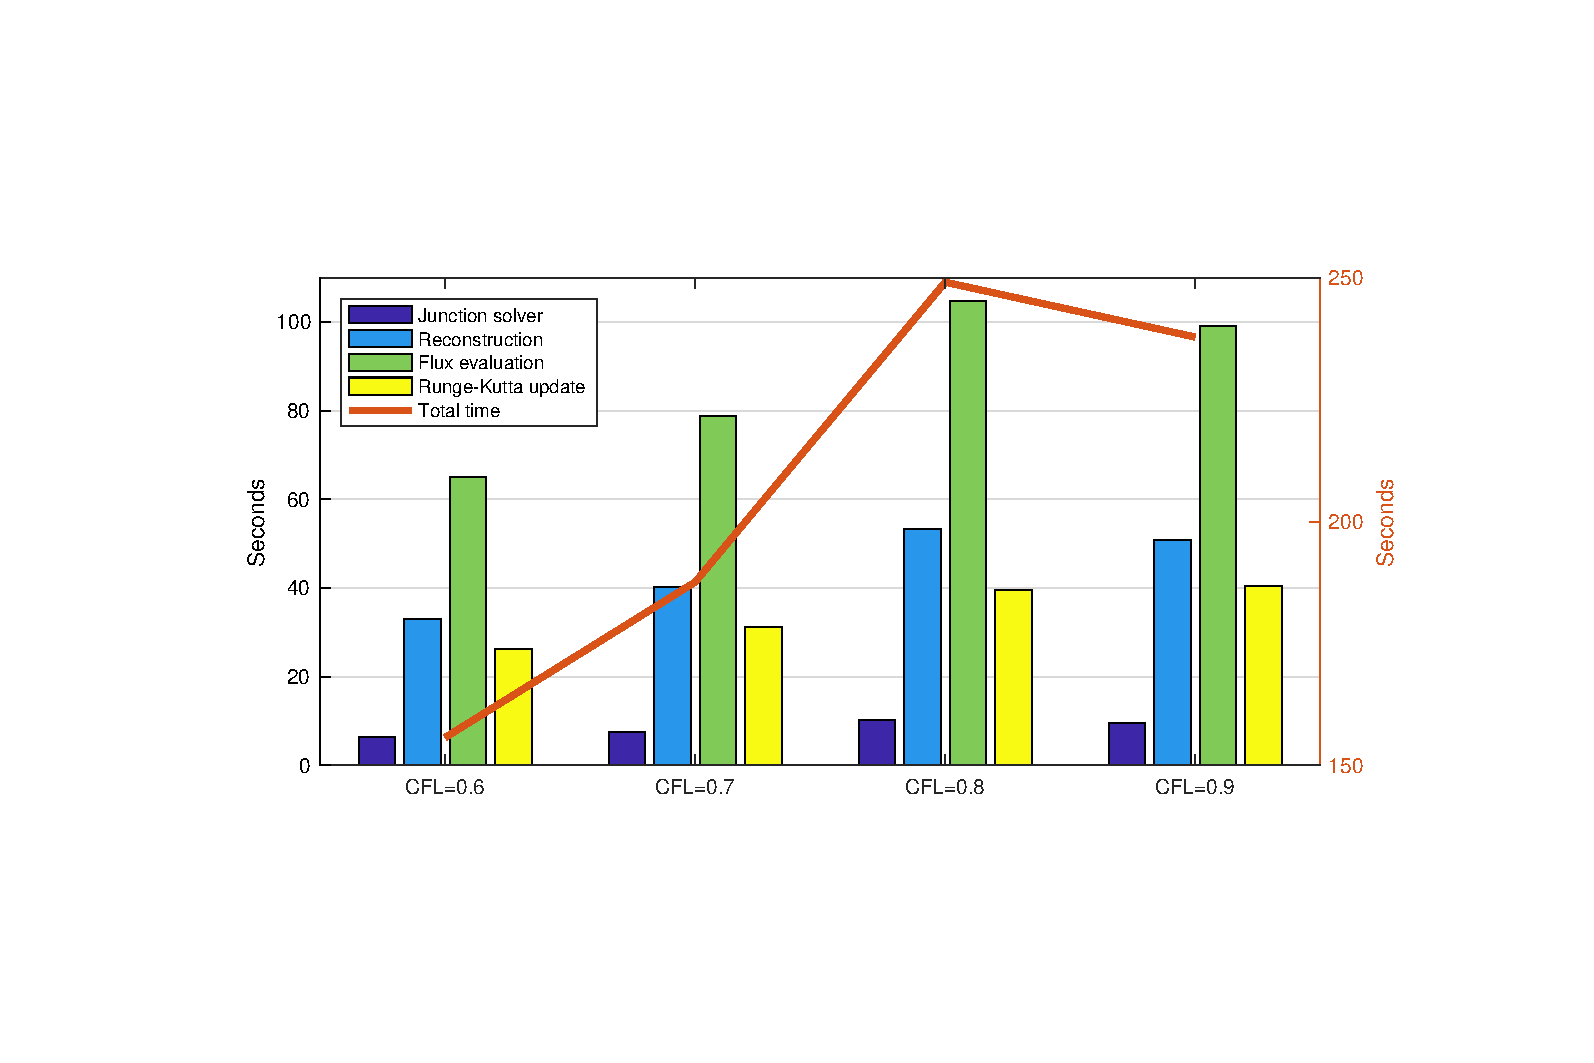
\includegraphics[trim=110 120 90 120,clip,width=\textwidth]{Time_M1J40_CFL.pdf}
		\caption[Time Analysis : M1J40 CFL]{Higher $CFL$ number increases computational time in total and is reflected over all timed segments of the code. The higher $CFL=0.8,0.9$ show a slightly opposite pattern. This information is joint with density profiles in Figure \ref{fig:randd:M1J40:cfl}.}
		\label{fig:randd:Time:M1J40_CFL}
	\end{figure}
	
	\begin{figure}
    		\centering
        		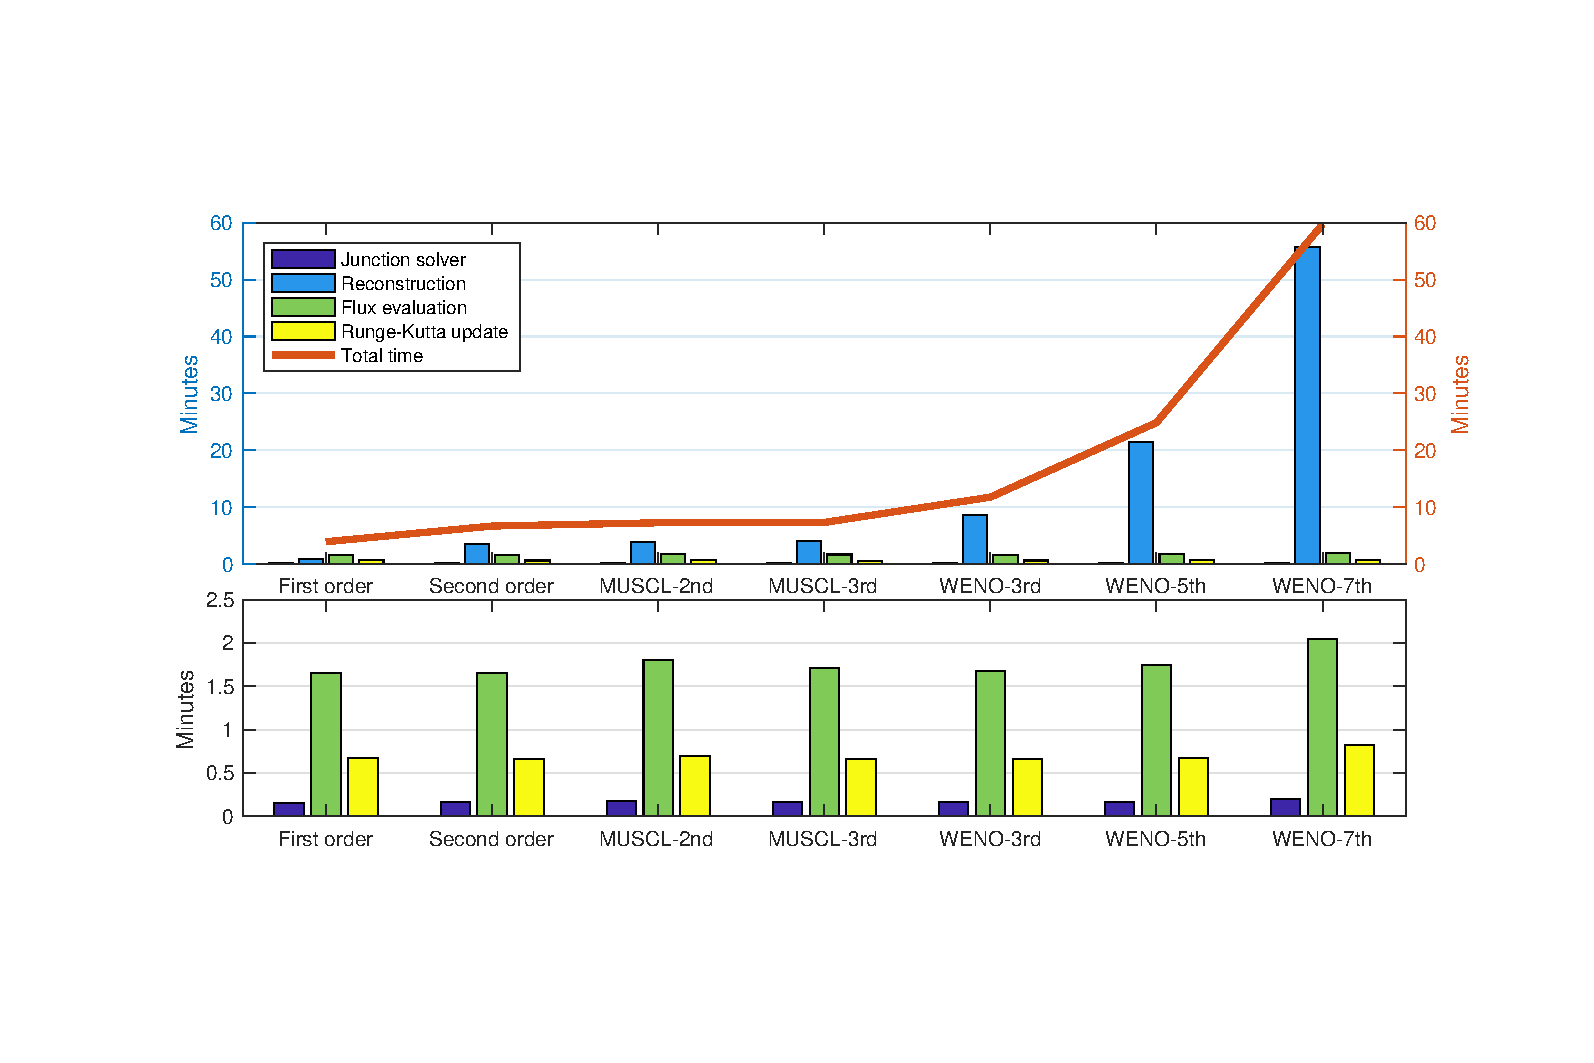
\includegraphics[trim=80 100 60 90,clip,width=\textwidth]{Time_M1J40_reco.pdf}
		\caption[Time Analysis : M1J40 reconstruction]{As reconstruction applies to every cell at every time step, any extra calculations computed as part of the reconstruction process scales with the number of spatial and time steps. Here it is clear that higher order reconstructions increase the reconstruction time (above), and the other simulation processes are unaffected by this (below). }
		\label{fig:randd:Time:M1J40_reco}
	\end{figure}
	
	\begin{figure}
    		\centering
        		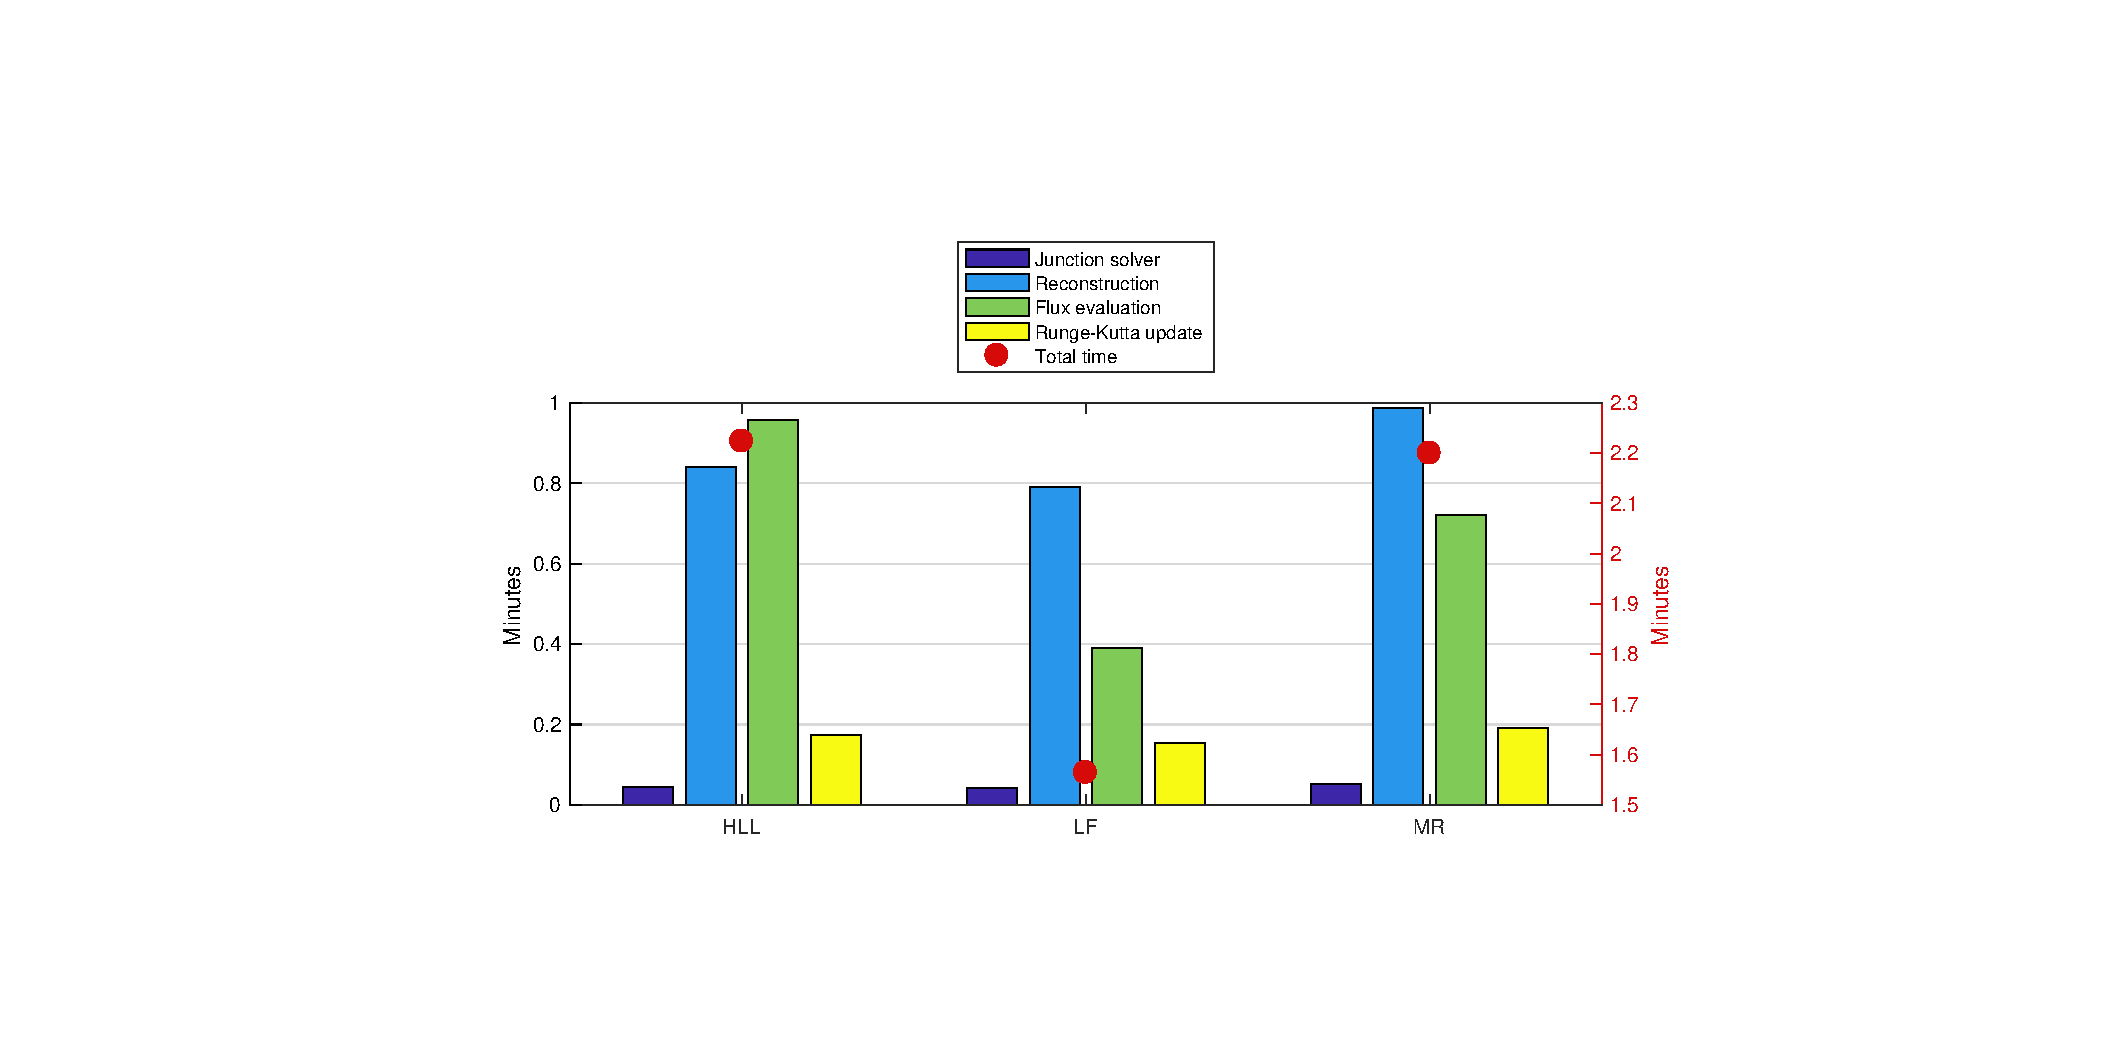
\includegraphics[trim=230 110 210 110,clip,width=0.85\textwidth]{Time_ReDiRoma_riem.pdf}
		\caption[Time Analysis : Re Di Roma Riemann solvers]{The Lax-Friedrichs solver is just over half as quick as the HLL and Murman-Roe solvers. If the choice of Riemann solver has little effect then it may be sensible to minimise computational time with the Lax-Friedrichs solver. }
		\label{fig:randd:Time:ReDiRoma:riem}
	\end{figure}
	
	\begin{figure}
    		\centering
        		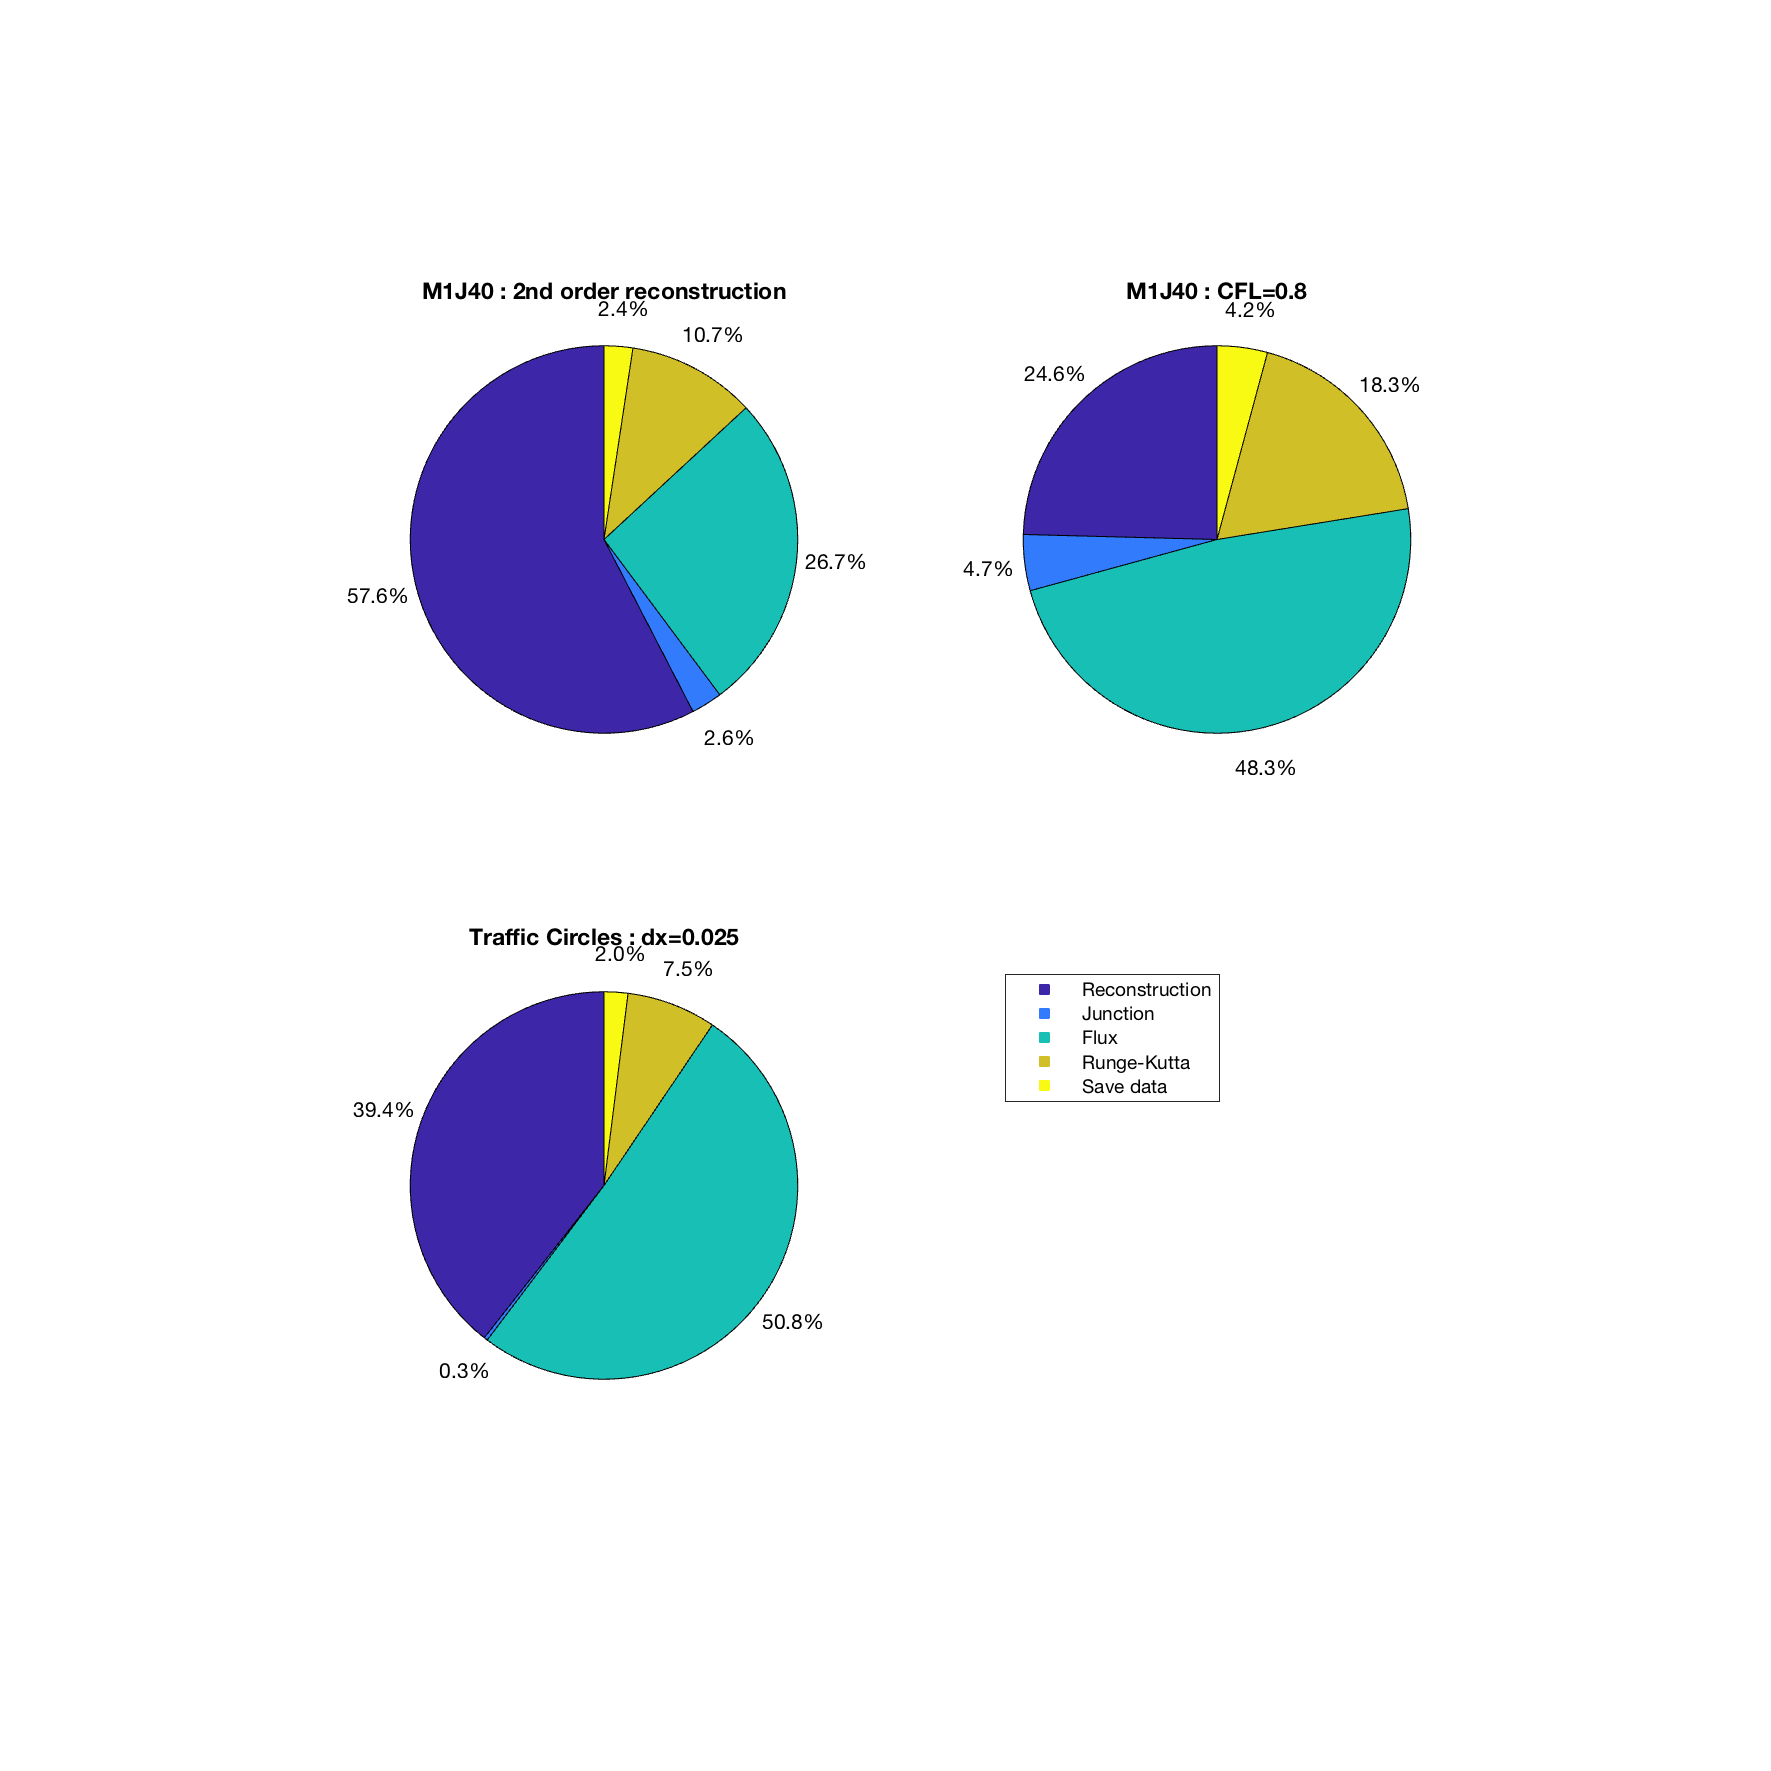
\includegraphics[trim=160 170 160 130,clip,width=0.85\textwidth]{Time_mixed.pdf}
		\caption[Time Analysis : Total time breakdown]{Depending on the choice of simulation parameters, the total simulation time is distributed varyingly over the sections shown in the above legend. For higher order reconstruction, this can dominate almost entirely, but other elements of the simulation are more time-influential with low order reconstructions.}
		\label{fig:randd:Time:mixed}
	\end{figure}
	
	
	
	
	
	
	
	
	\chapter{Final Remarks}
\label{ch:final}

\section{Conclusions}
\label{sec:conclusions}

	The following conclusions can be made about the topics covered:

	\begin{itemize}
		\item There are many approaches to solving compressible flow problems, different combinations of numerical schemes, Riemann solvers and slope limiters all interact and give varying solutions of common problems. Many researchers have reviewed existing methods and developed new ideas to combat the issues of previous schemes.
		\item The choice of numerical methods in traffic flow simulations is more significant with volatile flows changing quickly, in long simulations where flow changes are very gradual the effect of numerical methods are dulled.
		\item The general WENO scheme as presented in Appendix \ref{ap:WENOreco} cannot be extended to higher orders of $k\geq4$ without applying some bounding to preserve montonicity as in Appendix \ref{ap:monotonicitypreservingbounds} from Balsara and Shu \cite{BalsaraShu00}.
		\item From the analysis of MUSCL slope limiters in Figures \ref{fig:randd:traffic_circles:limiters} and \ref{fig:randd:Time:traffic_circles:limiters}, the VanLeer \cite{VanLeer74} limiter is identified as most advantageous, giving a high resolution solution of the density drop, a shorter computational cost, and with little $3^{rd}$ order speedup.
	\end{itemize}

\section{Further Ideas}
\label{sec:future}

The following recommendations are made for future research:
	
	\begin{itemize}
		\item More suitable parameters related to traffic flow quantities are required to be used as parameters for Riemann solvers to obtain varying results and to test which Riemann solvers are more or less appropriate for TFM. Once such parameters have been established, the HLLC solver (Appendix \ref{ap:HLLCriemann}) can be implemented and tested. 
		\item Improve MATLAB scripts to read in road network information to split up roads automatically depending on number of roads, their individual length and the spatial step $dx$.
		\item An interesting simulation may be over a long time period such as 24 hours with a time-dependent TDM, using the Wakefield M1 junction as a network.
		\item Revise the junction solver and check for conservation of density, aiming to investigate the spike of density shown in Figure \ref{fig:randd:M1J40:cfl} and \ref {fig:randd:M1J40:reco}.
		\item Implement and test some other stream models as listed in Section \ref{sec:streammodels}, to identify in which scenarios other stream models perform better. This test can be backed by some empirical data collected on real roads as has been done in the reviews \cite{ArdekaniGhandehariNepal11}, \cite{TiwariMarsani14}, \cite{LuMeng13}, \cite{Tom14}.
		\item A test of the suitability of the LWR model \cite{Lighthill55},\cite{Richards56} against the Payne-high-order model \cite{Payne71} and some empirical traffic data would be useful to investigate if it is the underlying mathematical description of traffic which influences a simulation results more than the chosen numerical methods to proceed through this description.
		\item Investigate the effect of other Runge-Kutta time update schemes against the classical fourth order method used here (Section \ref{sec:timeupdatescheme}). Runge-Kutta schemes can be written into an adaptive scheme by comparing a 7$^{th}$ and 8$^{th}$ order update (for example) for the error and adapting the time step accordingly, alternatively such as the third order stability preserving method used in \cite{ShiGuo16}, 
	\end{itemize}

%%%%%%%%%%%%%%%%%%%%%	
%%%%%%% End Matter %%%%%%%
%%%%%%%%%%%%%%%%%%%%%

\renewcommand\bibname{References}
\addcontentsline{toc}{chapter}{References}
\setstretch{1.18}
	\bibliography{references}
\setstretch{1}
\markboth{References}{}

\appendix

	\chapter{Computer Codes}
\label{ap:code}
\markboth{Computer Codes}{}
\graphicspath{{image_directory/appendix/}}
\lstset{inputpath=code/}


\section{Simulation Codes}
	
\subsection{\emph{main.py}}
\label{code:main} 
	\lstset{style=p}
	\lstinputlisting[firstline=0,lastline=863]{main.py}
	
\newpage

\subsection{\emph{define$\_$map.py}}
\label{code:definemap} 
	\lstset{style=p}
	\lstinputlisting[firstline=0,lastline=191]{define_map.py}
	
\newpage

\subsection{\emph{MUSCLReconstruction.py}}
\label{code:musclreconstruction} 
	\lstset{style=p}
	\lstinputlisting[firstline=0,lastline=194]{MUSCLReconstruction.py}
	
\newpage

\subsection{\emph{WENOReconstruction.py}}
\label{code:wenoreconstruction} 
	\lstset{style=p}
	\lstinputlisting[firstline=0,lastline=436]{WENOReconstruction.py}

\subsection{\emph{params.txt}}
\label{code:params} 
	\lstset{style=txt}
	\lstinputlisting[firstline=0,lastline=7]{params.txt}
	
\newpage

\section{MATLAB Postprocessing Codes}
\lstset{inputpath=code/MATLAB/}
\label{code:MATLABpostprocessing}

\subsection{Re Di Roma Roundabout}
\label{code:ReDiRoma}

\subsubsection{\emph{RomeRoundaboutPlot.m}}
	\lstset{style=m}
	\lstinputlisting[firstline=0,lastline=153]{RomeRoundaboutPlot.m}
	
\subsubsection{\emph{multicollineplot.m}}
\label{code:multicolline}
	\lstset{style=m}
	\lstinputlisting[firstline=0,lastline=18]{multicollineplot.m}
	
\newpage

\subsection{M1 Wakefield Junction 40}
\label{code:m1j40}

\subsubsection{\emph{M1J40plot.m}}

	\lstset{style=m}
	\lstinputlisting[firstline=0,lastline=233]{M1J40plot.m}
	
\subsubsection{\emph{arcpoints.m}}
\label{code:arcpoints}
	\lstset{style=m}
	\lstinputlisting[firstline=0,lastline=11]{arcpoints.m}
	
\newpage

\subsubsection{\emph{denlineplot.m}}
\label{code:denlineplot}
	\lstset{style=m}
	\lstinputlisting[firstline=0,lastline=27]{denlineplot.m}
	
\newpage
	
\section{Other Codes}

\subsection{Nagel-Schreckenberg Cellular Automation}
\lstset{inputpath=code/NS/}
\label{code:NaSc}

\subsubsection{\emph{NS$\_$implementation.m}}
	\lstset{style=m}
	\lstinputlisting[firstline=0,lastline=148]{NS_implementation.m}

\subsubsection{\emph{drawCircle.m}}
	\lstset{style=m}
	\lstinputlisting[firstline=0,lastline=10]{drawCircle.m}
		

	
	\chapter{Higher Order Reconstruction Procedures}
\label{ap:reco}
\markboth{Higher Order Reconstruction Procedures}{}
\graphicspath{{image_directory/appendix/}}

\section{MUSCL}
\label{ap:MUSCLreco}

	For the single cell $i$, the left and right reconstructed states are given by $\rho^{R}_{i-1/2}$ and $\rho_{i+1/2}^{L}$ respectively. 

\subsection{Linear - 2nd Order}
	
	The 2nd order MUSCL scheme approximates the cell density distribution with a linear slope. The left and right states are given by
	\begin{align}
		\rho^{R}_{i-1/2}&=\rho_i-\frac{1}{2}\phi\left(r_i\right)\left(\rho_{i+1}-\rho_{i}\right),\\
		\rho^{L}_{i+1/2}&=\rho_i+\frac{1}{2}\phi\left(r_i\right)\left(\rho_{i+1}-\rho_{i}\right),
	\end{align}
	where 
	\begin{equation}
		r_{i}=\frac{\rho_{i}-\rho_{i-1}}{\rho_{i+1}-\rho_{i}},
	\end{equation}
	and $\phi$ is the slope limiting function.
	
	\begin{figure}
    		\centering
        		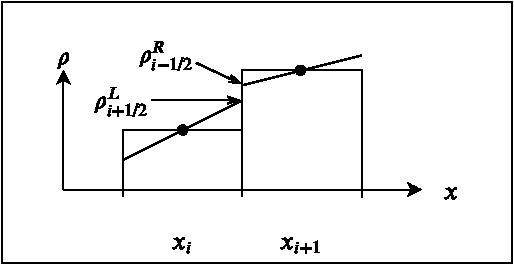
\includegraphics[trim=20 5 20 20,clip,width=0.6\textwidth]{MUSCL_linear.pdf}
		\caption[MUSCL Reconstruction : Linear $2^{nd}$ order]{MUSCL second order piecewise linear reconstruction.}
		\label{fig:app:muscl_lin}
	\end{figure}
	
\subsection{Parabolic - 3rd Order}

	The 3rd order MUSCL scheme approximates the cell density distribution with a parabolic slope, from a second order interpolation. The left and right states are given by
	\begin{align}
		\rho^{R}_{i-1/2}&=\rho_{i}-\frac{1}{4}\phi\left(r_{i}\right)\left[\left(1-\kappa\right)\delta\rho_{i+1/2}+\left(1+\kappa\right)\delta\rho_{i-1/2}\right],\\
		\rho^{L}_{i+1/2}&=\rho_{i}+\frac{1}{4}\phi\left(r_{i}\right)\left[\left(1-\kappa\right)\delta\rho_{i-1/2}+\left(1+\kappa\right)\delta\rho_{i+1/2}\right],
	\end{align}
	with $\kappa=1/3$, $\delta\rho_{i+1/2}=\rho_{i+1}-\rho_{i}$, $\delta\rho_{i-1/2}=\rho_{i}-\rho_{i-1}$, and the slope limiter $\phi$.
	
	\begin{figure}
    		\centering
        		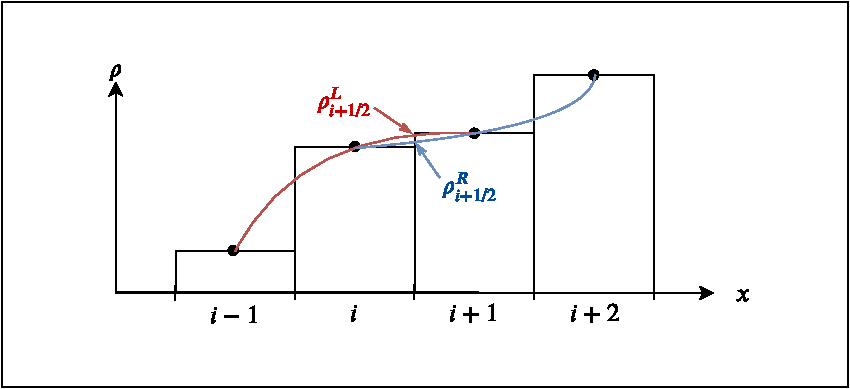
\includegraphics[trim=40 30 40 30,clip,width=0.7\textwidth]{MUSCL_para.pdf}
		\caption[MUSCL Reconstruction : Parabolic $3^{rd}$ order]{MUSCL third order piecewise parabolic reconstruction using second order interpolation.}
		\label{fig:app:muscl_para}
	\end{figure}
	
\subsection{Slope Limiters}
\label{ap:MUSCLslopelim}

	The listed slope limiters apply to MUSCL reconstructions to reduce cell interface oscillations. All present limiters are written in \emph{MUSCLReconstruction.py}, Appendix  \ref{code:musclreconstruction} [lines 90-185].
	
	\begin{itemize}
	
		\item CHARM [not 2nd order TVD] \cite{Zhou95}
			\begin{equation}
				\phi\left(r\right)=
				\begin{cases}
					\frac{r\left(3r+1\right)}{\left(r+1\right)^2},    &r>0\\
					0,  &r\leq0
				\end{cases}
			\end{equation}
			
		\item HCUS [not 2nd order TVD] \cite{Waterson95}
			\begin{equation}
				\phi\left(r\right)=\frac{3\left(r+\left|r\right|\right)}{2\left(r+2\right)}
			\end{equation}
			
		\item HQUICK [not 2nd order TVD] \cite{Waterson95}
			\begin{equation}
				\phi\left(r\right)=\frac{2\left(r+\left|r\right|\right)}{\left(r+3\right)}
			\end{equation}
			
		\item Koren [3rd order TDV accurate for sufficiently smooth data] \cite{Koren93}
			\begin{equation}
				\phi\left(r\right)=\max\left[0,\min\left(2r,\min\left(\frac{1+2r}{3},2\right)\right)\right]
			\end{equation}
			
		\item MinMod [2rd order TDV accurate] \cite{Roe86}
			\begin{equation}
				\phi\left(r\right)=\max\left[0,\min\left(1,r\right)\right]
			\end{equation}
			
		\item Monotonized Central (MC) [2rd order TDV accurate, symmetric] \cite{VanLeer77}
			\begin{equation}
				\phi\left(r\right)=\max\left[0,\min\left(2r, \frac{1+r}{2},2\right)\right]
			\end{equation}
			
		\item Osher [2rd order TDV accurate] \cite{Osher83}
			\begin{equation}
				\phi\left(r\right)=\max\left[0,\min\left(r,\beta\right)\right], \quad\left(1\leq\beta\leq2\right)
			\end{equation}
			
		\item Ospre [2rd order TDV accurate, symmetric] \cite{Waterson95}
			\begin{equation}
				\phi\left(r\right)=\frac{3\left(r^2+r\right)}{2\left(r^2+r+1\right)}
			\end{equation}
			
		\item Smart [not 2rd order TDV] \cite{Gaskell88}
			\begin{equation}
				\phi\left(r\right)=\max\left[0,\min\left(2r,\frac{1+3r}{4},4\right)\right]
			\end{equation}
			
		\item Superbee [2rd order TDV accurate, symmetric] \cite{Roe86}
			\begin{equation}
				\phi\left(r\right)=\max\left[0,\min\left(2r,1\right),\min\left(r,2\right)\right]
			\end{equation}
			
		\item Sweby [not 2rd order TDV, symmetric] \cite{Sweby84}
			\begin{equation}
				\phi\left(r\right)=\max\left[0,\min\left(\beta r,1\right),\min\left(r,\beta\right)\right], \quad\left(1\leq\beta\leq2\right)
			\end{equation}
			
		\item UMIST [2rd order TDV accurate] \cite{Lien94}
			\begin{equation}
				\phi\left(r\right)=\max\left[0,\min\left(2r,\frac{1+3r}{4},\frac{3+r}{4},2\right)\right]
			\end{equation}
			
			\newpage
			
		\item van Albada 1 [2rd order TDV accurate, symmetric] \cite{VanAlbada82}
			\begin{equation}
				\phi\left(r\right)=\frac{r^2+r}{r^2+1}
			\end{equation}
			
		\item van Albada 2 - alternate form for high spatial order schemes [not 2rd order TDV] \cite{Kermani03}
			\begin{equation}
				\phi\left(r\right)=\frac{2r}{r^2+1}
			\end{equation}
			
		\item van Leer [2nd order TVD accurate, symmetric] \cite{VanLeer74}
			\begin{equation}
				\phi\left(r\right)=\frac{r+\left|r\right|}{1+\left|r\right|}
			\end{equation}
	
	\end{itemize}
	
	\subsection*{Other Limiters}

	To calculate the gradient limiter, Barth and Jesperson \cite{Barth89} suggested using $\Phi_i=\min\left(\Phi_{ij}\right)$, where
	\begin{equation}
		\Phi_{ij}=
		\begin{cases}
			\min\left(1,\frac{\delta \rho_i^{\max}}{\rho_{ij}-\overline{\rho}_i}\right), & if \quad \rho_{ij}-\overline{\rho}_i>0, \\
			\min\left(1,\frac{\delta \rho_i^{\min}}{\rho_{ij}-\overline{\rho}_i}\right), & if \quad \rho_{ij}-\overline{\rho}_i<0,\\
			1, & if \quad \rho_{ij}-\overline{\rho}_i=0.
		\end{cases}
		\nonumber
	\end{equation}
	The values $\delta \rho_i^{\max}$ and $\delta \rho_i^{\min}$ are the maximum and minimum of $\overline{\rho}-\overline{\rho}_i$ respectively, the difference between the concerned volume and nearest neighbours. The value, $\rho_{ij}=R_i\left(\vec{x}_j-\vec{x}_i\right)$, is the unlimited reconstructed value. Due to the minimum, maximum, and case selections of $\Phi_i$ in the Barth and Jespersen limiter, the reconstructed flux is non-differentiable, which slows the solving convergence. Venkatakrishnan \cite{Venkatakrishnan93} suggested a smooth approximation of the case selection step in the Barth and Jespersen limiter. This approximation uses $\phi(r)$ instead of $\min(1,r)$, where 
	\begin{equation}
		\phi(r)=\frac{r^2+2r}{r^2+r+2}, \label{eq:ven_approx}
	\end{equation}
	so for $\rho_{ij}-\overline{\rho}_i<0$
	\begin{equation}
		\Phi_{ij}=\phi\left(\frac{\delta \rho_i^{\min}}{\rho_{ij}-\overline{\rho}_i}\right). \nonumber
	\end{equation}
	Venkatakrishnan also suggested avoiding the limiter for regions of uniform flow, i.e. when $\rho_{ij}-\overline{\rho}_i>0$
	\begin{equation}
		\Phi_{ij}=\frac{1}{\Delta_-}\left[\frac{\left(\Delta_+^2+\epsilon^2\right)\Delta_-+2\Delta_-^2\Delta_+}{\Delta_+^2+2\Delta_-^2+\Delta_-\Delta_++\epsilon^2}\right], \nonumber
	\end{equation}
	where $\Delta_-=\rho_{ij}-\overline{\rho}_i$, $\Delta_+=\delta \rho_i^{\max}$, and $\epsilon^2=\left(K\Delta x\right)^3$ with parameter $K>0$. The case for $\rho_{ij}-\overline{\rho}_i=0$ remains unchanged with $\Phi_{ij}=1$.
	
	\begin{figure}
    		\centering
        		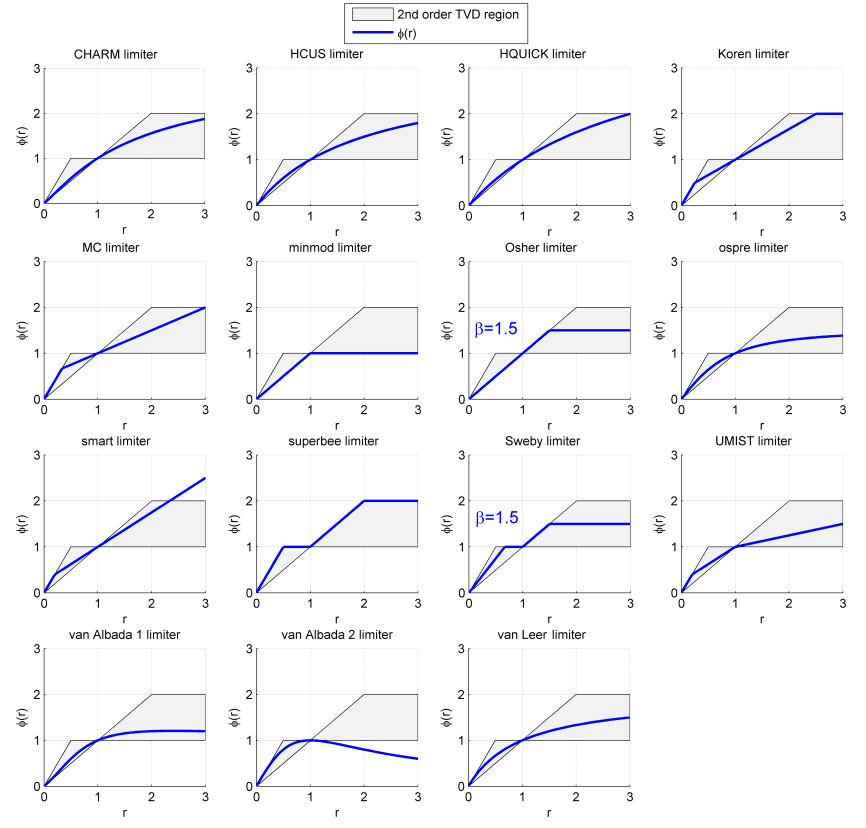
\includegraphics[trim=0 0 0 0,clip,width=\textwidth]{Limiters.png}
		\caption[MUSCL Reconstruction : Slope limiters]{Plots showing the slope limiter $\phi(r)$ on $r\geq0$ over the admissible TVD region for second order schemes \cite{Sweby84}. Created in MATLAB \cite{Griffgruff}.}
		\label{fig:app:slopelims}
	\end{figure}
	

\section{WENO}
\label{ap:WENOreco}

	The general $\left(2k-1\right)^{th}$ order WENO reconstruction considers a convex combination of $k$ reconstructions from unique local stencils. See \cite{Shu97} for a more thorough discussion and derivation of WENO and ENO schemes, Procedure 2.2 provides the general WENO scheme steps presented here. The available $3^{rd}$, $5^{th}$, and $7^{th}$ order reconstructions in \emph{WENOReconstruction.py} \ref{code:wenoreconstruction} are represented by $k=2,3,4$ respectively. For cell $i$, we want approximations for the left, $\rho^{+}_{i-1/2}$, and right, $\rho^{-}_{i+1/2}$, density values. The following steps provide an algorithm for computing the WENO reconstructed cell interface values to the required order.
\begin{enumerate}
	\item Consider the $k$ stencils over $x_{i-(k-1)},\hdots,x_{i+(k-1)}$, denoted by $S_r$ for $r=0,\hdots,k-1$,
		\begin{equation}
			S_r=\left\{x_{i-r}, x_{i-r+1},\hdots,x_{i-r+(k-1)}\right\}.
		\end{equation}
	\item Obtain $k$ \emph{right} and $k$ \emph{left} reconstructed values,
		\begin{equation}
			\rho^{(r)}_{i+1/2}=\sum_{j=0}^{k-1}c_{r,j}\overline\rho_{i-r+j},\quad\text{and},\quad \rho^{(r)}_{i-1/2}=\sum_{j=0}^{k-1}\tilde c_{r,j}\overline\rho_{i-r+j}
		\end{equation}
		using the cell averaged density values $\overline\rho$, and weights $c_{r,j}$ and $\tilde c_{r,j}$ with $\tilde c_{r,j}=c_{r-1,j}$ ($r=-1$ is provided for the left-right transformation purposes) where $c_{r,j}$ are
		\begin{center}
			\begin{tabular}{|c|c|cccc|}
				\hline
 				\multirow{2}{*}{$k$} & \multirow{2}{*}{$r$} & \multicolumn{4}{c|}{$j$} \\
 				 & & 0 & 1 & 2 & 3 \\
 				 \hline
 				\multirow{2}{*}{$2$} & -1 & 3/2 & -1/2 & - & - \\
 				& 0 & 1/2 & 1/2 & - & - \\
 				& 1 & -1/2 & 3/2 & - & - \\
 				 \hline
 				\multirow{3}{*}{$3$} & -1 & 11/6 & -7/6 & 1/3 & - \\
 				& 0 & 1/3 & 5/6 & -1/6 & - \\
 				& 1 & -1/6 & 5/6 & 1/3 & - \\
 				& 2 & 1/3 & -7/6 & 11/6 & - \\
 				\hline
 				\multirow{4}{*}{$4$} & -1 & 25/12 & -23/12 & 13/12 & -1/4 \\
 				& 0 & 1/4 & 13/12 & -5/12 & 1/12 \\
 				& 1 & -1/12 & 7/12 & 7/12 & -1/12 \\
 				& 2 & 1/12 & -5/12 & 13/12 & 1/4 \\
 				& 3 & -1/4 & 13/12 & -23/12 & 25/12 \\
 				\hline
			\end{tabular}
		\end{center}
	
	\item Define the constants $d_r$ and $\tilde d_r=d_{k-1-r}$
		\begin{center}
			\begin{tabular}{|c|ccc|}
				\hline
				\multirow{2}{*}{$r$} & \multicolumn{3}{c|}{$k$}\\
				& 2 & 3 & 4 \\
				\hline
				0 & 2/3 & 3/10 & 4/35\\
				1 & 1/3 & 3/5 & 18/35\\
				2 & - & 1/10 & 12/35\\
				3 & - & - & 1/35\\
				\hline
			\end{tabular}
		\end{center}
	
	\item Find the smoothness indicators. For $k=2$ these can be written in a simple form
		\begin{equation}
			\beta_r=\left(\overline\rho_{i+1-r}-\overline\rho_{i-r}\right)^2.
		\end{equation}
		The smoothness indicator form for $k=3$ is
		\begin{equation}
			\beta_r = \frac{13}{12}\left(\sum_{j=0}^{k-1}b^{(0)}_{r,j}\overline\rho_{i-r+j}\right)^2+\frac{1}{4}\left(\sum_{j=0}^{k-1}b^{(1)}_{r,j}\overline\rho_{i-r+j}\right)^2,
		\end{equation}
		with coefficients as below.
		\begin{center}
			\begin{tabular}{|c|ccc|ccc|}
				\hline
				 \multirow{2}{*}{$r$} & \multicolumn{3}{|c|}{$b^{(0)}$ : $j$} & \multicolumn{3}{|c|}{$b^{(1)}$ : $j$}\\
				 & 0 & 1 & 2 & 0 & 1 & 2\\
				 \hline
				 0 & 1 & -2 & 1 & 3 & -4 & 1\\
				 1 & 1 & -2 & 1 & 1 & 0 & -1\\
				 2 & 1 & -2 & 1 & 1 & -4 & 3\\
				\hline
			\end{tabular}
		\end{center}
		For higher order WENO schemes, the smoothness factors of which are of the form \cite{BalsaraShu00}
		\begin{equation}
			\beta_r = \sum^{k-1}_{j=0}\left[\overline\rho_{i-r+j}\cdot\left(\sum_{g=0}^{k-1-j}\hat{b}_{r,j,g}\cdot\overline\rho_{i-r+j+g}\right)\right]
		\end{equation}
		with $\hat{b}_{r,j,g}$ from
		\begin{center}
			\begin{tabular}{|c|c|cccc|}
			\hline
				 \multirow{2}{*}{$r$} & \multirow{2}{*}{$j$} & \multicolumn{4}{c|}{$g$} \\
				  & & 0 & 1 & 2 & 3 \\
			\hline
				 \multirow{4}{*}{$0$}  & 0 & 2107 & -9402 & 7042 & -1854 \\
				                                      & 1 & 11003 & -17246 & 4642 & - \\
				                                      & 2 & 7043 & -3882 & - & - \\
				                                      & 3 & 547 & - & - & - \\
			\hline
				 \multirow{4}{*}{$1$}  & 0 & 547 & -2522 & 1922 & -494 \\
				                                      & 1 & 3443 & -5966 & 1602 & - \\
				                                      & 2 & 2843 & -1642 & - & - \\
				                                      & 3 & 267 & - & - & - \\
			\hline
				 \multirow{4}{*}{$2$}  & 0 & 267 & -1642 & 1602 & -494 \\
				                                      & 1 & 2843 & -5966 & 1922 & - \\
				                                      & 2 & 3443 & -2522 & - & - \\
				                                      & 3 & 547 & - & - & - \\
			\hline
				 \multirow{4}{*}{$3$}  & 0 & 547 & -3882 & 4642 & -1854 \\
				                                      & 1 & 7043 & -17246 & 7042 & - \\
				                                      & 2 & 11003 & -9402 & - & - \\
				                                      & 3 & 2107 & - & - & - \\
			\hline
			\end{tabular}
		\end{center}
		using the cell averaged density values $\overline\rho$.
		
	\item[5a] Calculate alpha weights
		\begin{align}
			\tilde\alpha_r&=\frac{\tilde d_r}{\left(\epsilon+\beta_r\right)^2},\\
			\alpha_r&=\frac{d_r}{\left(\epsilon+\beta_r\right)^2},
		\end{align}
		using the weights $d$ from step 3, and the smoothness indicators $\beta$ from step 4. The constant $\epsilon=10^{-6}$ to avoid a division by zero.
		
	\item[5b] Calculate the omega weights
		\begin{align}
			\tilde\omega_r&=\frac{\tilde\alpha_r}{\tilde\alpha_0+\tilde\alpha_1+\tilde\alpha_2}, \\
			\omega_r&=\frac{\alpha_r}{\alpha_0+\alpha_1+\alpha_2},
		\end{align}
		using the weights $\alpha$ from step 5a.
		
	\item[6] Evaluate the final interface reconstructions
		\begin{align}
			\rho^{-}_{i+1/2}&=\sum_{j=0}^{k-1}\omega_j\rho^{(j)}_{i+1/2}, \\
			\rho^{+}_{i-1/2}&=\sum_{j=0}^{k-1}\tilde\omega_j\rho^{(j)}_{i-1/2},
		\end{align}
		using the weights $\omega$ from step 5b, and the polynomial reconstructed values $\rho_{i\pm1/2}^{(r)}$ from step 2.
\end{enumerate}

	\begin{figure}
    		\centering
        		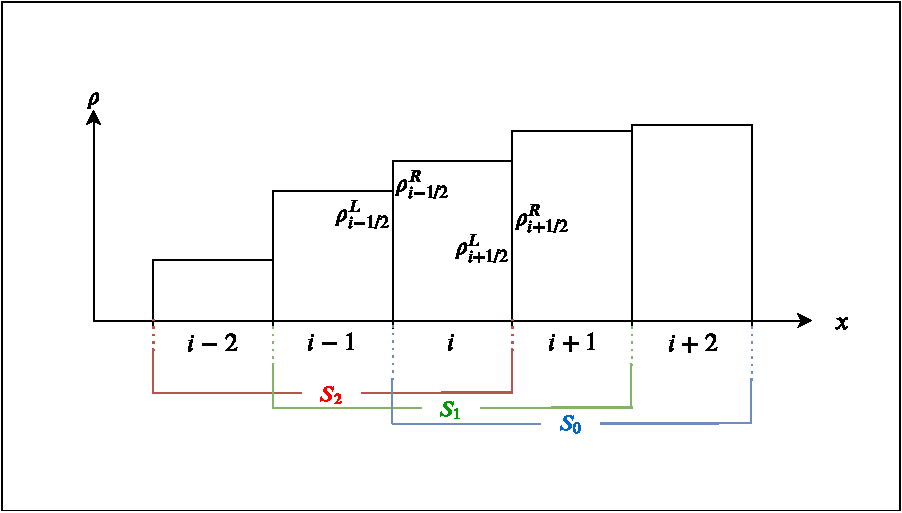
\includegraphics[trim=35 35 20 40,clip,width=\textwidth]{WENO5.pdf}
		\caption[WENO reconstruction stencil]{WENO stencil.}
		\label{fig:app:weno}
	\end{figure}
	
\subsection{Monotonicity Preserving Bounds}
\label{ap:monotonicitypreservingbounds}

	Proposing an improvement on Suresh and Huynh \cite{Suresh97}, Balsara and Shu \cite{BalsaraShu00} give a method to monotonically bound the reconstructed states. Suresh and Huynh \cite{Suresh97} found that bounding local extrema reduces the order of accuracy and should be avoided for higher order schemes. The following presents a scheme for the monotonicity preserving bound proposed in \cite{BalsaraShu00}. This method is applied to the $7^{th}$ order WENO reconstruction in Appendix \ref{code:wenoreconstruction}. Begin by defining the minmod and median functions,
	\begin{align}	
		\mathrm{minmod}(x,y)&=\frac{1}{2}\left(\mathrm{sign}(x)+\mathrm{sign}(y)\right)\min\left(|x|,|y|\right),\\
		\mathrm{median}(x,y,z)&=x+\mathrm{minmod}(y-x,z-x).
	\end{align}
	In alignment with the the substeps $a$ to $e$ of step 7 in the WENO code in Appendix \ref{code:wenoreconstruction}, step $7a$ defines the local curvature measures $d_j,d_{j+1},d_{j-1}$ similarly by
	\begin{equation}
		d_j=\rho_{j+1}-2\rho_{j}+\rho_{j-1}.
	\end{equation}
	Step $7b$ improves on Suresh and Huynh \cite{Suresh97} by taking the minmod, allowing local extrema to develop,
	\begin{equation}
		\rho_{j+1/2}^{MM}=\mathrm{minmod}(d_j,d_{j+1}).
	\end{equation}
	As well as the minmod evaluation (denoted in the superscript $MM$), an allowance is made for large curvature ($LC$) controlled by the parameter $\beta$. Step $7c$ defines $\beta$ and $\alpha$ two curvature constant parameters. The value of $\beta$ determines the freedom from allowing a large local curvature , and $\alpha$ determines the appropriate CFL number. Suresh and Huynh \cite{Suresh97} claim setting $\alpha=2$ and $\beta=4$ allow a CFL of at least 0.6 and do not degrade the monotonicity preserving property. Step $7d$ define the median ($MD$), upper limit ($UL$) and large curvature ($LC$) density solutions. The following provide definitions for the right states, the left can be evaluated symmetrically,
	\begin{align}
		\rho_{j+1/2}^{MD}&=\frac{1}{2}\left(\rho_j+\rho_{j+1}\right)-\frac{1}{2}d_{j+1/2}^{MD},\\
		\rho_{j+1/2}^{UL}&=\rho_j+\alpha\left(\rho_j-\rho_{j-1}\right),\\
		\rho_{j+1/2}^{LC}&=\rho_j+\frac{1}{2}\left(\rho_j-\rho_{j-1}\right)+\frac{\beta}{3}d_{j-1/2}^{LC}.
	\end{align}
	Step $7e$ defines new bounds for the maximum and minimum reconstructed states before computing the monotonicity preserving value.
	\begin{align}
		\rho_{j+1/2}^{L,\min}&=\max\left\{\min\left(\rho_j,\rho_{j+1},\rho_{j+1/2}^{MD}\right),\min\left(\rho_j,\rho_{j+1/2}^{UL},\rho_{j+1/2}^{LC}\right)\right\},\\
		\rho_{j+1/2}^{L,\max}&=\min\left\{\max\left(\rho_j,\rho_{j+1},\rho_{j+1/2}^{MD}\right),\max\left(\rho_j,\rho_{j+1/2}^{UL},\rho_{j+1/2}^{LC}\right)\right\}.
	\end{align}
	Finally the monotonicity preserving bounds are calculated and returned as outputs of the WENO function,
	\begin{equation}
		\rho_{j+1/2}^L=\mathrm{median}(\rho^L_{j+1/2},\rho^{L,\min}_{j+1/2},\rho^{L,\max}_{j+1/2}).
	\end{equation}
	Within this approach there are many outcomes achieved by setting $d^{MD}$, $d^{LC}$, $d^{MM}$ equal in various combinations. The paper from Balsara and Shu \cite{BalsaraShu00} tests these monotonicity preserving bounds on standard hyperbolic test cases. 
	













	
	\chapter{Supplementary Material}
\label{ap:supp}
\markboth{Supplementary Material}{}
\graphicspath{{image_directory/appendix/}}

\section{HLLC Riemann Solver}
\label{ap:HLLCriemann}

	In 1992 Toro \cite{Toro92} introduced a development of the HLL Riemann solver, assuming the two original waves present in HLL and inbetween adding in a contact wave\footnote{The C in HLLC stands for contact wave.}.The HLLC fluxes are also given depending on the choice of left and right wave speeds as well as an middle speed given as $S_*$. The HLLC flux is given by four regions separated by three waves,
	\begin{equation}
		\mathbf{F}=
		\begin{cases}
			\mathbf{F}_L, & if \quad 0\leq S_L, \\
			\mathbf{F}_{*L}=\mathbf{F}_L+S_L\left(\mathbf{U}_{*L}-\mathbf{U}_L\right), & if \quad S_L\leq0\leq S_*, \\
			\mathbf{F}_{*R}=\mathbf{F}_R+S_R\left(\mathbf{U}_{*R}-\mathbf{U}_R\right), & if \quad S_*\leq0\leq S_R, \\
			\mathbf{F}_R, & if \quad S_R\leq0.
		\end{cases}
		\nonumber
	\end{equation}
	The middle conserved vector $\mathbf{U}_{*K}$, for $K=L,R$, is expressed in 1D as
	\begin{equation}
		\mathbf{U}_{*K}^{1D}=\rho_K\left(\frac{S_K-u_K}{S_K-S_*}\right)
		\left[
		\begin{matrix}
			1\\
			S_*\\
			\frac{E_K}{\rho_K}+\left(S_*-u_K\right)\left(S_*+\frac{p_K}{\rho_K\left(S_K-u_K\right)}\right)
		\end{matrix}
		\right],
		\nonumber
	\end{equation}
	and in 2D as
	\begin{equation}
		\mathbf{U}_{*K}^{2D}=\rho_K\left(\frac{S_K-u_K}{S_K-S_*}\right)
		\left[
		\begin{matrix}
			1\\
			S_*\\
			v_K \\
			\frac{E_K}{\rho_K}+\left(S_*-u_K\right)\left(S_*+\frac{p_K}{\rho_K\left(S_K-u_K\right)}\right)
		\end{matrix}
		\right].
		\nonumber
	\end{equation}
	The middle wave speed $S_*$ depends on the dimension of the problem, for 1D
	\begin{equation}
		S_*^{1D}=\frac{p_R-p_L+\rho_Lu_L\left(S_L-u_L\right)-\rho_Ru_R\left(S_R-u_R\right)}{\rho_L\left(S_L-u_L\right)-\rho_R\left(S_R-u_R\right)}, \nonumber
	\end{equation}
	however in 2D, the approximate Riemann solver has the conditions \cite{Toro09},
	\begin{equation}
		u_{*L}=u_{*R}=u_*, \quad and \quad S_*=u_*, \nonumber
	\end{equation}
	so the middle wave speed in 2D is
	\begin{equation}
		S_*^{2D}=u_*. \nonumber
	\end{equation}
	All flow variables in the left or right states, including left and right fluxes, can be calculated from the variables given in the conserved vector $\mathbf{U}$.

\section{Nagel-Schreckenberg Model}
\label{ap:nagsch}

	See Section \ref{sec:nagschreck}, and code in Appendix \ref{code:NaSc}.

	\begin{figure}[H]
  		\centering
  		\subfloat[Physical location]{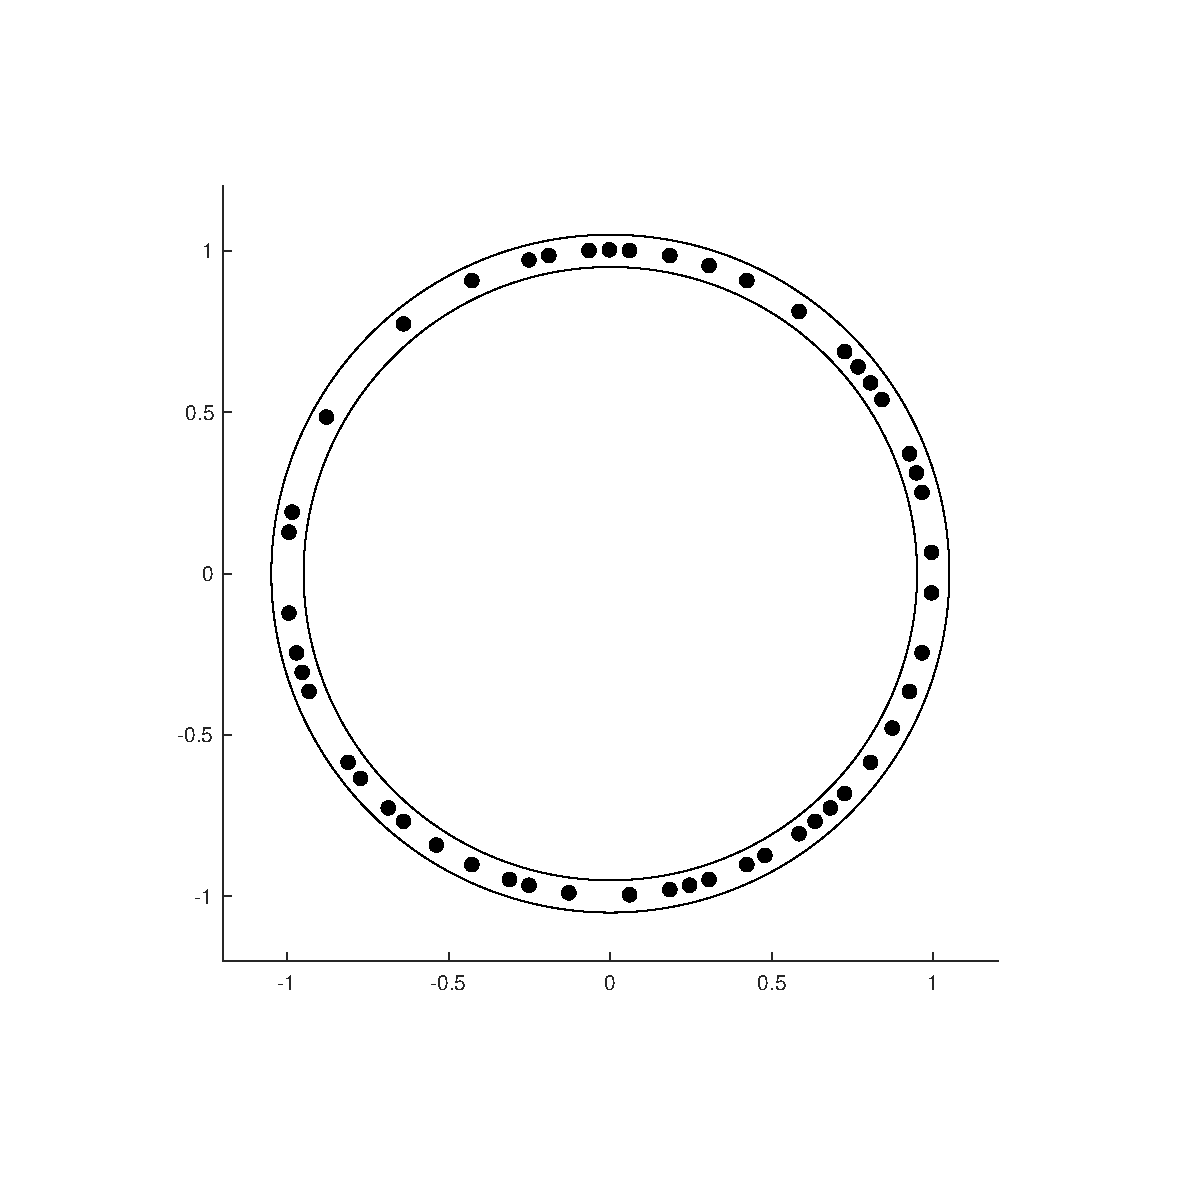
\includegraphics[trim=50 70 60 70,clip,width=0.49\textwidth]{NS_physical.pdf}\label{fig:supp:NaSc:phys}}
  		\hfill
  		\subfloat[Pathline clustering waves]{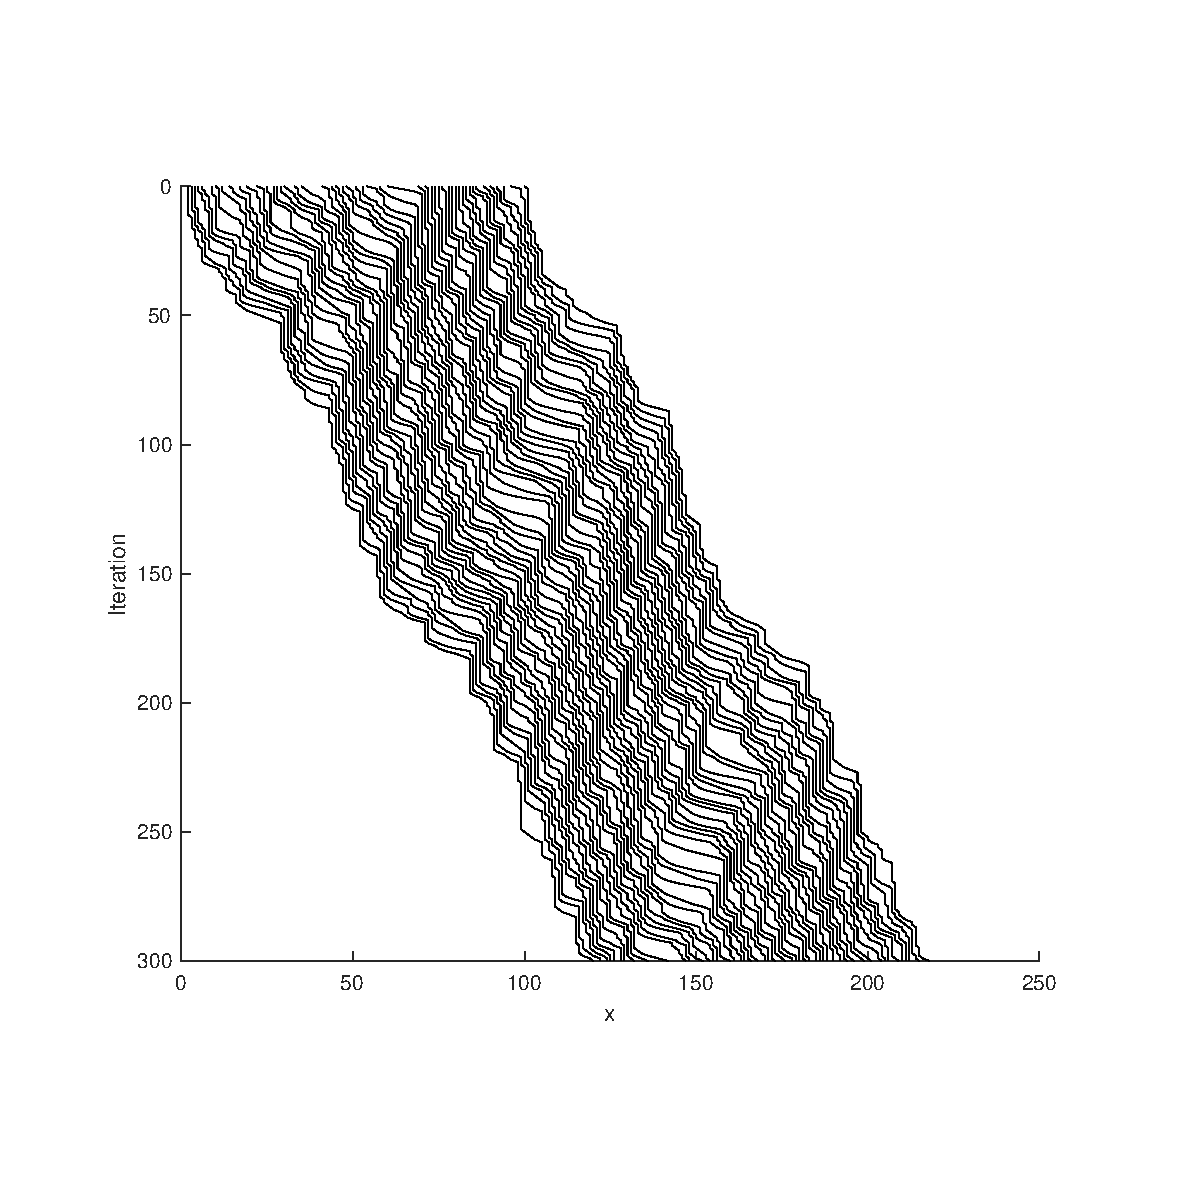
\includegraphics[trim=50 70 60 70,clip,width=0.49\textwidth]{NS_waves.pdf}\label{fig:supp:NaSc:wav}}
  		\caption[Nagel-Schreckenberg simulation]{Results from 300 iterations of the Nagel-Schreckenberg \cite{Nagel92} model. Figures show physical position on a circular road (a), and displacement $x$ from the road origin traced by iteration to show phantom traffic jams. \label{fig:aupp:NaSc}}
	\end{figure}

\newpage
\section{Genealogical Traffic Flow Model Tree}

	\begin{figure}[H]
    		\centering
        		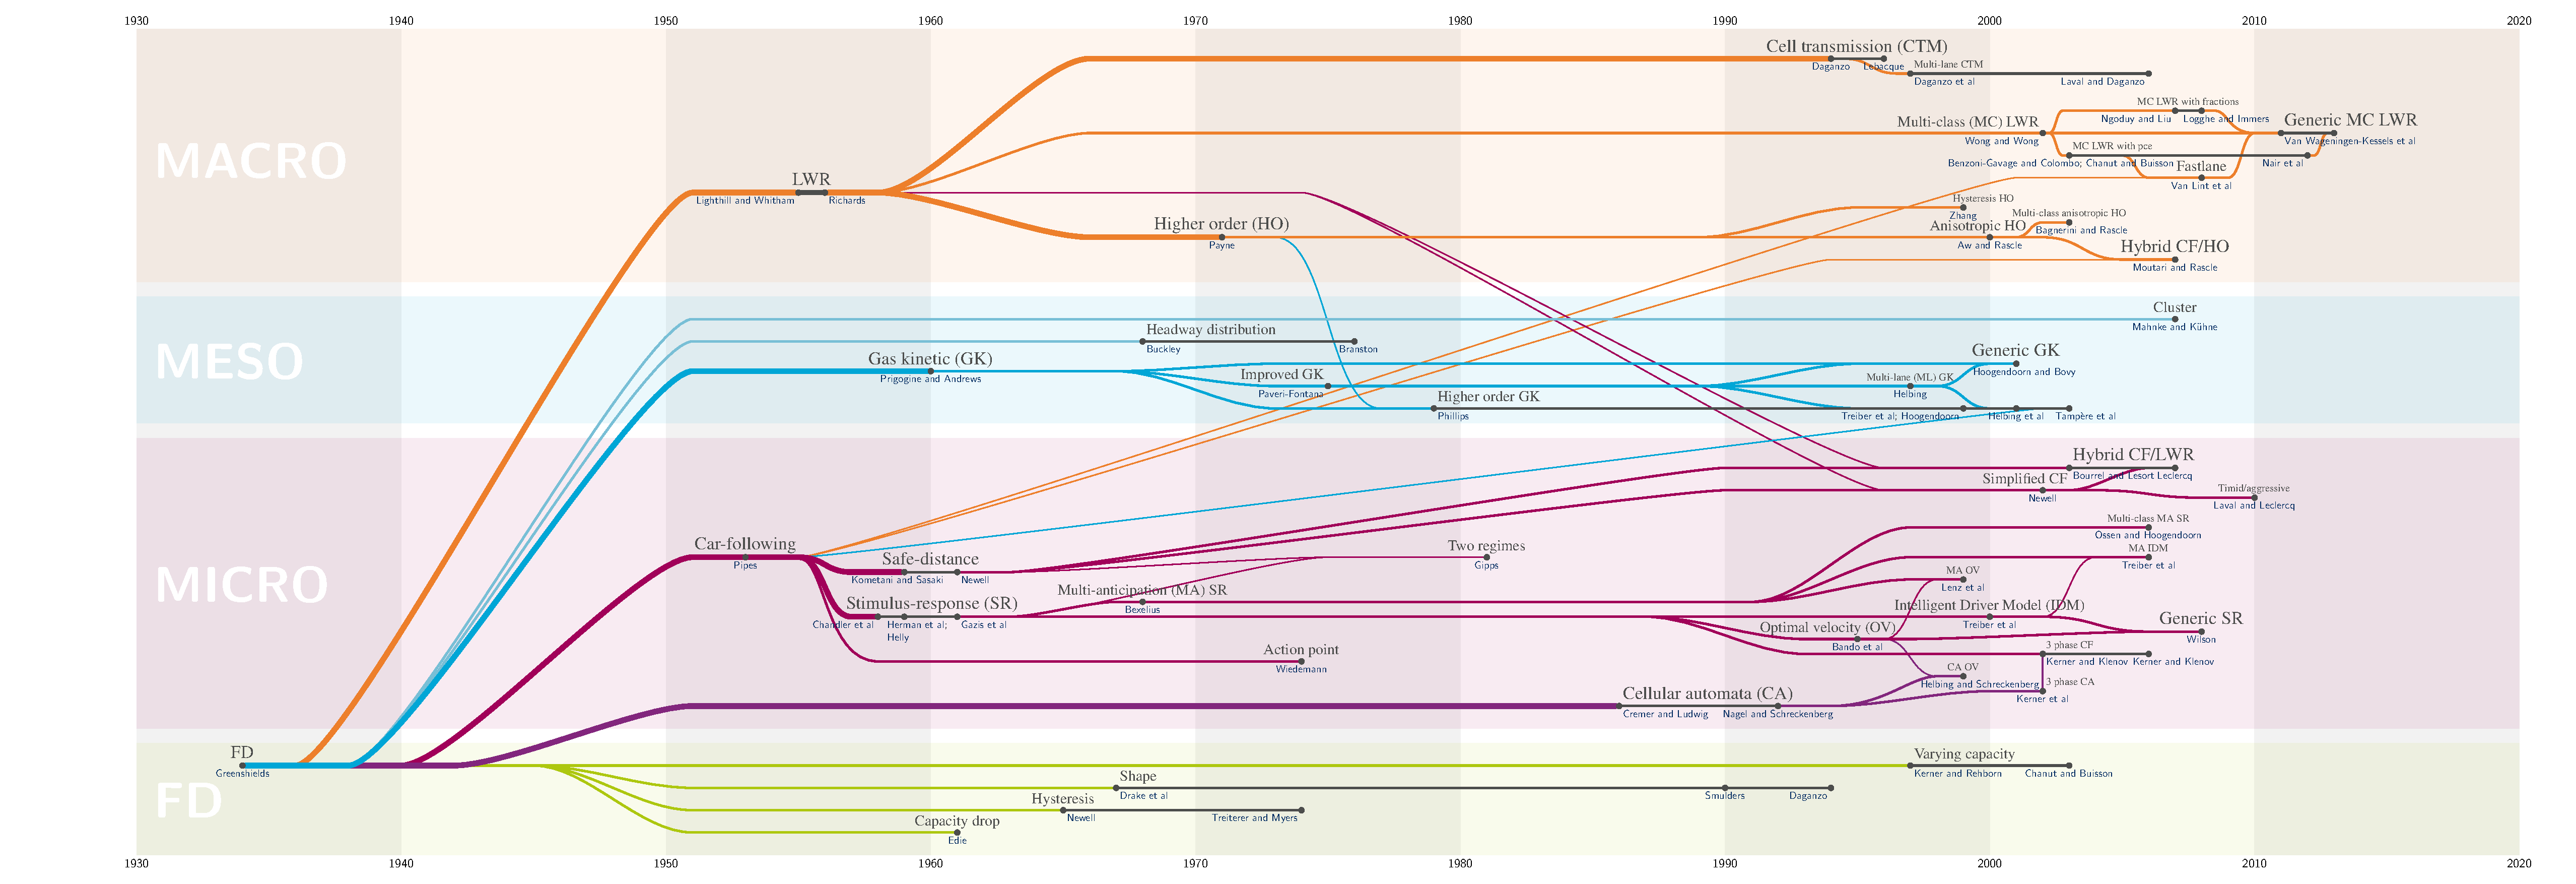
\includegraphics[angle=90,origin=c,trim=0 0 0 0,clip,height=0.9\textwidth]{TFM_timeline.pdf}
		\caption[Genealogical model tree]{Part of the online access \cite{Kessels15} (doi: \href{https://doi.org/10.1007/s13676-014-0045-5}{\texttt{10.1007/s13676-014-0045-5}}) includes a full size version complete with references.}
		\label{fig:supp:tree}
	\end{figure}
	
\newpage
\section{Simulation Information Output}
\lstset{inputpath=textfiles/}
\label{txt:info:output} 

\subsection{Written Text File}
\label{txt:info:file} 
	\lstset{style=txt}
	\lstinputlisting[firstline=0,lastline=49]{simulation_info.txt}

\subsection{Console}
\label{txt:info:console} 
	\lstset{style=txt}
	\lstinputlisting[firstline=0,lastline=8]{console.txt}








	
\createblankpage
\createblankpage
% end on a blank even page

\end{document}
